% Created 2020-10-28 三 15:25
% Intended LaTeX compiler: pdflatex
\documentclass{article}
\usepackage[utf8]{inputenc}
\usepackage[T1]{fontenc}
\usepackage{graphicx}
\usepackage{grffile}
\usepackage{longtable}
\usepackage{wrapfig}
\usepackage{rotating}
\usepackage[normalem]{ulem}
\usepackage{amsmath}
\usepackage{textcomp}
\usepackage{amssymb}
\usepackage{capt-of}
\usepackage{hyperref}
%%%%%%%%%%%%%%%%%%%%%%%%%%%%%%%%%%%%%%
%% TIPS                                 %%
%%%%%%%%%%%%%%%%%%%%%%%%%%%%%%%%%%%%%%
% \substack{a\\b} for multiple lines text

\usepackage[utf8]{inputenc}

\usepackage[B1,T1]{fontenc}

% pdfplots will load xolor automatically without option
\usepackage[dvipsnames]{xcolor}
%%%%%%%%%%%%%%%%%%%%%%%%%%%%%%%%%%%%%%%
%% MATH related pacakge                  %%
%%%%%%%%%%%%%%%%%%%%%%%%%%%%%%%%%%%%%%%
% \usepackage{amsmath} mathtools loads the amsmath
\usepackage{amsmath}
\usepackage{mathtools}


\usepackage{amsthm}
\usepackage{amsbsy}

%\usepackage{commath}

\usepackage{amssymb}
\usepackage{mathrsfs}
%\usepackage{mathabx}
\usepackage{stmaryrd}
\usepackage{empheq}

\usepackage{scalerel}
\usepackage{stackengine}
\usepackage{stackrel}

\usepackage{nicematrix}
\usepackage{tensor}
\usepackage{blkarray}
\usepackage{siunitx}
\usepackage[f]{esvect}

\usepackage{unicode-math}
\setmainfont{TeX Gyre Pagella}
% \setmathfont{STIX}
% \setmathfont{texgyrepagella-math.otf}
% \setmathfont{Libertinus Math}
\setmathfont{Latin Modern Math}
\setmathfont[range={\mscra,\mscrb,\mscrc,\mscrd,\mscre,\mscrf,\mscrg,\mscrh,\mscri,\mscrj,\mscrk,\mscrl,\mscrm,\mscrn,\mscro,\mscrp,\mscrq,\mscrr,\mscrs,\mscrt,\mscru,\mscrv,\mscrw,\mscrx,\mscry,\mscrz,\mscrA,\mscrB,\mscrC,\mscrD,\mscrE,\mscrF,\mscrG,\mscrH,\mscrI,\mscrJ,\mscrK,\mscrL,\mscrM,\mscrN,\mscrO,\mscrP,\mscrQ,\mscrR,\mscrS,\mscrT,\mscrU,\mscrV,\mscrW,\mscrX,\mscrY,\mscrZ}]{Latin Modern Math}
\setmathfont[range={\smwhtdiamond,\enclosediamond,\varlrtriangle}]{Latin Modern Math}
\setmathfont[range={\rightrightarrows,\twoheadrightarrow,\leftrightsquigarrow,\triangledown}]{XITS Math}
\setmathfont[range={\int,\setminus}]{Libertinus Math}



%%%%%%%%%%%%%%%%%%%%%%%%%%%%%%%%%%%%%%%
%% TIKZ related packages                 %%
%%%%%%%%%%%%%%%%%%%%%%%%%%%%%%%%%%%%%%%

\usepackage{pgfplots}
\pgfplotsset{compat=1.15}
\usepackage{tikz}
\usepackage{tikz-cd}
\usepackage{tikz-qtree}

\usetikzlibrary{arrows,positioning,calc,fadings,decorations,matrix,decorations,shapes.misc}
%setting from geogebra
\definecolor{ccqqqq}{rgb}{0.8,0,0}


%%%%%%%%%%%%%%%%%%%%%%%%%%%%%%%%%%%%%%%
%% MISCLELLANEOUS packages               %%
%%%%%%%%%%%%%%%%%%%%%%%%%%%%%%%%%%%%%%%
\usepackage[most]{tcolorbox}
\usepackage{threeparttable}
\usepackage{tabularx}

\usepackage{enumitem}

% wrong with preview
\usepackage{subcaption}
\usepackage{caption}
% {\aunclfamily\Huge}
\usepackage{auncial}

\usepackage{float}

\usepackage{fancyhdr}

\usepackage{ifthen}
\usepackage{xargs}


\usepackage{imakeidx}
\usepackage{hyperref}
\usepackage{soul}


%\usepackage[xetex]{preview}
%%%%%%%%%%%%%%%%%%%%%%%%%%%%%%%%%%%%%%%
%% USEPACKAGES end                       %%
%%%%%%%%%%%%%%%%%%%%%%%%%%%%%%%%%%%%%%%

% \setlist{nosep}
% \numberwithin{equation}{subsection}
% \fancyhead{} % Clear the headers
% \renewcommand{\headrulewidth}{0pt} % Width of line at top of page
% \fancyhead[R]{\slshape\leftmark} % Mark right [R] of page with Chapter name [\leftmark]
% \pagestyle{fancy} % Set default style for all content pages (not TOC, etc)


% \newlength\shlength
% \newcommand\vect[2][0]{\setlength\shlength{#1pt}%
%   \stackengine{-5.6pt}{$#2$}{\smash{$\kern\shlength%
%     \stackengine{7.55pt}{$\mathchar"017E$}%
%       {\rule{\widthof{$#2$}}{.57pt}\kern.4pt}{O}{r}{F}{F}{L}\kern-\shlength$}}%
%       {O}{c}{F}{T}{S}}


\indexsetup{othercode=\small}
\makeindex[columns=2,options={-s /media/wu/file/stuuudy/notes/index_style.ist},intoc]
\makeatletter
\def\@idxitem{\par\hangindent 0pt}
\makeatother


%\newcounter{dummy} \numberwithin{dummy}{section}
\newtheorem{dummy}{dummy}[section]
\theoremstyle{definition}
\newtheorem{definition}[dummy]{Definition}
\theoremstyle{plain}
\newtheorem{corollary}[dummy]{Corollary}
\newtheorem{lemma}[dummy]{Lemma}
\newtheorem{proposition}[dummy]{Proposition}
\newtheorem{theorem}[dummy]{Theorem}
\theoremstyle{definition}
\newtheorem{examplle}{Example}[section]
\theoremstyle{remark}
\newtheorem*{remark}{Remark}
\newtheorem{exercise}{Exercise}[subsection]
\newtheorem{observation}{Observation}[section]


\newenvironment{claim}[1]{\par\noindent\textbf{Claim:}\space#1}{}

\makeatletter
\DeclareFontFamily{U}{tipa}{}
\DeclareFontShape{U}{tipa}{m}{n}{<->tipa10}{}
\newcommand{\arc@char}{{\usefont{U}{tipa}{m}{n}\symbol{62}}}%

\newcommand{\arc}[1]{\mathpalette\arc@arc{#1}}

\newcommand{\arc@arc}[2]{%
  \sbox0{$\m@th#1#2$}%
  \vbox{
    \hbox{\resizebox{\wd0}{\height}{\arc@char}}
    \nointerlineskip
    \box0
  }%
}
\makeatother

\setcounter{MaxMatrixCols}{20}
%%%%%%% ABS
\DeclarePairedDelimiter\abss{\lvert}{\rvert}%
\DeclarePairedDelimiter\normm{\lVert}{\rVert}%

% Swap the definition of \abs* and \norm*, so that \abs
% and \norm resizes the size of the brackets, and the
% starred version does not.
\makeatletter
\let\oldabs\abss
%\def\abs{\@ifstar{\oldabs}{\oldabs*}}
\newcommand{\abs}{\@ifstar{\oldabs}{\oldabs*}}
\newcommand{\norm}[1]{\left\lVert#1\right\rVert}
%\let\oldnorm\normm
%\def\norm{\@ifstar{\oldnorm}{\oldnorm*}}
%\renewcommand{norm}{\@ifstar{\oldnorm}{\oldnorm*}}
\makeatother

% \newcommand\what[1]{\ThisStyle{%
%     \setbox0=\hbox{$\SavedStyle#1$}%
%     \stackengine{-1.0\ht0+.5pt}{$\SavedStyle#1$}{%
%       \stretchto{\scaleto{\SavedStyle\mkern.15mu\char'136}{2.6\wd0}}{1.4\ht0}%
%     }{O}{c}{F}{T}{S}%
%   }
% }

% \newcommand\wtilde[1]{\ThisStyle{%
%     \setbox0=\hbox{$\SavedStyle#1$}%
%     \stackengine{-.1\LMpt}{$\SavedStyle#1$}{%
%       \stretchto{\scaleto{\SavedStyle\mkern.2mu\AC}{.5150\wd0}}{.6\ht0}%
%     }{O}{c}{F}{T}{S}%
%   }
% }

% \newcommand\wbar[1]{\ThisStyle{%
%     \setbox0=\hbox{$\SavedStyle#1$}%
%     \stackengine{.5pt+\LMpt}{$\SavedStyle#1$}{%
%       \rule{\wd0}{\dimexpr.3\LMpt+.3pt}%
%     }{O}{c}{F}{T}{S}%
%   }
% }

\newcommand{\bl}[1] {\boldsymbol{#1}}
\newcommand{\Wt}[1] {\stackrel{\sim}{\smash{#1}\rule{0pt}{1.1ex}}}
\newcommand{\wt}[1] {\widetilde{#1}}
\newcommand{\tf}[1] {\textbf{#1}}


%For boxed texts in align, use Aboxed{}
%otherwise use boxed{}

\DeclareMathSymbol{\widehatsym}{\mathord}{largesymbols}{"62}
\newcommand\lowerwidehatsym{%
  \text{\smash{\raisebox{-1.3ex}{%
    $\widehatsym$}}}}
\newcommand\fixwidehat[1]{%
  \mathchoice
    {\accentset{\displaystyle\lowerwidehatsym}{#1}}
    {\accentset{\textstyle\lowerwidehatsym}{#1}}
    {\accentset{\scriptstyle\lowerwidehatsym}{#1}}
    {\accentset{\scriptscriptstyle\lowerwidehatsym}{#1}}
  }


\newcommand{\cupdot}{\mathbin{\dot{\cup}}}
\newcommand{\bigcupdot}{\mathop{\dot{\bigcup}}}

\usepackage{graphicx}

\usepackage[toc,page]{appendix}

% text on arrow for xRightarrow
\makeatletter
%\newcommand{\xRightarrow}[2][]{\ext@arrow 0359\Rightarrowfill@{#1}{#2}}
\makeatother

% Arbitrary long arrow
\newcommand{\Rarrow}[1]{%
\parbox{#1}{\tikz{\draw[->](0,0)--(#1,0);}}
}

\newcommand{\LRarrow}[1]{%
\parbox{#1}{\tikz{\draw[<->](0,0)--(#1,0);}}
}


\makeatletter
\providecommand*{\rmodels}{%
  \mathrel{%
    \mathpalette\@rmodels\models
  }%
}
\newcommand*{\@rmodels}[2]{%
  \reflectbox{$\m@th#1#2$}%
}
\makeatother







\newcommand{\trcl}[1]{%
  \mathrm{trcl}{(#1)}
}



% Roman numerals
\makeatletter
\newcommand*{\rom}[1]{\expandafter\@slowromancap\romannumeral #1@}
\makeatother
% \\def \\b\([a-zA-Z]\) {\\boldsymbol{[a-zA-z]}}
% \\DeclareMathOperator{\\b\1}{\\textbf{\1}}


\DeclareMathOperator{\bx}{\textbf{x}}
\DeclareMathOperator{\bz}{\textbf{z}}
\DeclareMathOperator{\bff}{\textbf{f}}
\DeclareMathOperator{\ba}{\textbf{a}}
\DeclareMathOperator{\bk}{\textbf{k}}
\DeclareMathOperator{\bs}{\textbf{s}}
\DeclareMathOperator{\bh}{\textbf{h}}
\DeclareMathOperator{\bc}{\textbf{c}}
\DeclareMathOperator{\br}{\textbf{r}}
\DeclareMathOperator{\bi}{\textbf{i}}
\DeclareMathOperator{\bj}{\textbf{j}}
\DeclareMathOperator{\bn}{\textbf{n}}
\DeclareMathOperator{\be}{\textbf{e}}
\DeclareMathOperator{\bo}{\textbf{o}}
\DeclareMathOperator{\bU}{\textbf{U}}
\DeclareMathOperator{\bL}{\textbf{L}}
\DeclareMathOperator{\bV}{\textbf{V}}
\def \bzero {\mathbf{0}}
\def \btwo {\mathbf{2}}
\DeclareMathOperator{\bv}{\textbf{v}}
\DeclareMathOperator{\bp}{\textbf{p}}
\DeclareMathOperator{\bI}{\textbf{I}}
\DeclareMathOperator{\bM}{\textbf{M}}
\DeclareMathOperator{\bN}{\textbf{N}}
\DeclareMathOperator{\bK}{\textbf{K}}
\DeclareMathOperator{\bt}{\textbf{t}}
\DeclareMathOperator{\bb}{\textbf{b}}
\DeclareMathOperator{\bA}{\textbf{A}}
\DeclareMathOperator{\bX}{\textbf{X}}
\DeclareMathOperator{\bu}{\textbf{u}}
\DeclareMathOperator{\bS}{\textbf{S}}
\DeclareMathOperator{\bZ}{\textbf{Z}}
\DeclareMathOperator{\by}{\textbf{y}}
\DeclareMathOperator{\bw}{\textbf{w}}
\DeclareMathOperator{\bT}{\textbf{T}}
\DeclareMathOperator{\bF}{\textbf{F}}
\DeclareMathOperator{\bmm}{\textbf{m}}
\DeclareMathOperator{\bW}{\textbf{W}}
\DeclareMathOperator{\bR}{\textbf{R}}
\DeclareMathOperator{\bC}{\textbf{C}}
\DeclareMathOperator{\bD}{\textbf{D}}
\DeclareMathOperator{\bE}{\textbf{E}}
\DeclareMathOperator{\bQ}{\textbf{Q}}
\DeclareMathOperator{\bP}{\textbf{P}}
\DeclareMathOperator{\bY}{\textbf{Y}}
\DeclareMathOperator{\bH}{\textbf{H}}
\DeclareMathOperator{\bB}{\textbf{B}}
\DeclareMathOperator{\bG}{\textbf{G}}
\def \blambda {\symbf{\lambda}}
\def \boldeta {\symbf{\eta}}
\def \balpha {\symbf{\alpha}}
\def \bbeta {\symbf{\beta}}
\def \bgamma {\symbf{\gamma}}
\def \bxi {\symbf{\xi}}
\def \bLambda {\symbf{\Lambda}}

\newcommand{\bto}{{\boldsymbol{\to}}}
\newcommand{\Ra}{\Rightarrow}
\newcommand\und[1]{\underline{#1}}
\def \bPhi {\boldsymbol{\Phi}}
\def \btheta {\boldsymbol{\theta}}
\def \bTheta {\boldsymbol{\Theta}}
\def \bmu {\boldsymbol{\mu}}
\def \bphi {\boldsymbol{\phi}}
\def \bSigma {\boldsymbol{\Sigma}}
\def \lb {\left\{}
\def \rb {\right\}}
\def \la {\langle}
\def \ra {\rangle}
\def \caln {\mathcal{N}}
\def \dissum {\displaystyle\Sigma}
\def \dispro {\displaystyle\prod}
\def \E {\mathbb{E}}
\def \Q {\mathbb{Q}}
\def \N {\mathbb{N}}
\def \V {\mathbb{V}}
\def \R {\mathbb{R}}
\def \P {\mathbb{P}}
\def \A {\mathbb{A}}
\def \F {\mathbb{F}}
\def \Z {\mathbb{Z}}
\def \I {\mathbb{I}}
\def \C {\mathbb{C}}
\def \cala {\mathcal{A}}
\def \cale {\mathcal{E}}
\def \calb {\mathcal{B}}
\def \calq {\mathcal{Q}}
\def \calp {\mathcal{P}}
\def \cals {\mathcal{S}}
\def \calx {\mathcal{X}}
\def \caly {\mathcal{Y}}
\def \calg {\mathcal{G}}
\def \cald {\mathcal{D}}
\def \caln {\mathcal{N}}
\def \calr {\mathcal{R}}
\def \calt {\mathcal{T}}
\def \calm {\mathcal{M}}
\def \calw {\mathcal{W}}
\def \calc {\mathcal{C}}
\def \calv {\mathcal{V}}
\def \calf {\mathcal{F}}
\def \calk {\mathcal{K}}
\def \call {\mathcal{L}}
\def \calu {\mathcal{U}}
\def \calo {\mathcal{O}}
\def \calh {\mathcal{H}}
\def \cali {\mathcal{I}}

\def \bcup {\bigcup}

% set theory

\def \zfcc {\textbf{ZFC}^-}
\def \ac  {\textbf{AC}}
\def \gl  {\textbf{L }}
\def \gll {\textbf{L}}
\newcommand{\zfm}{$\textbf{ZF}^-$}

%\def \zfm {$\textbf{ZF}^-$}
\def \zfmm {\textbf{ZF}^-}
\def \wf {\textbf{WF }}
\def \on {\textbf{On }}
\def \cm {\textbf{M }}
\def \cn {\textbf{N }}
\def \cv {\textbf{V }}
\def \zc {\textbf{ZC }}
\def \zcm {\textbf{ZC}}
\def \zff {\textbf{ZF}}
\def \wfm {\textbf{WF}}
\def \onm {\textbf{On}}
\def \cmm {\textbf{M}}
\def \cnm {\textbf{N}}
\def \cvm {\textbf{V}}
\def \gchh {\textbf{GCH}}
\renewcommand{\restriction}{\mathord{\upharpoonright}}
\def \pred {\text{pred}}

\def \rank {\text{rank}}
\def \con {\text{Con}}
\def \deff {\text{Def}}


\def \uin {\underline{\in}}
\def \oin {\overline{\in}}
\def \uR {\underline{R}}
\def \oR {\overline{R}}
\def \uP {\underline{P}}
\def \oP {\overline{P}}

\def \Ra {\Rightarrow}

\def \e {\enspace}

\def \sgn {\operatorname{sgn}}
\def \gen {\operatorname{gen}}
\def \Hom {\operatorname{Hom}}
\def \hom {\operatorname{hom}}
\def \Sub {\operatorname{Sub}}

\def \supp {\operatorname{supp}}

\def \epiarrow {\twoheadarrow}
\def \monoarrow {\rightarrowtail}
\def \rrarrow {\rightrightarrows}

% \def \minus {\text{-}}
% \newcommand{\minus}{\scalebox{0.75}[1.0]{$-$}}
% \DeclareUnicodeCharacter{002D}{\minus}


\def \tril {\triangleleft}

\def \ACF {\text{ACF}}
\def \GL {\text{GL}}
\def \PGL {\text{PGL}}
\def \equal {=}
\def \deg {\text{deg}}
\def \degree {\text{degree}}
\def \app {\text{App}}
\def \FV {\text{FV}}
\def \conv {\text{conv}}
\def \cont {\text{cont}}
\DeclareMathOperator{\cl}{\textbf{CL}}
\DeclareMathOperator{\sg}{sg}
\DeclareMathOperator{\trdeg}{trdeg}
\def \Ord {\text{Ord}}

\DeclareMathOperator{\cf}{cf}
\DeclareMathOperator{\zfc}{ZFC}

%\DeclareMathOperator{\Th}{Th}
%\def \th {\text{Th}}
% \newcommand{\th}{\text{Th}}
\DeclareMathOperator{\type}{type}
\DeclareMathOperator{\zf}{\textbf{ZF}}
\def \fa {\mathfrak{a}}
\def \fb {\mathfrak{b}}
\def \fc {\mathfrak{c}}
\def \fd {\mathfrak{d}}
\def \fe {\mathfrak{e}}
\def \ff {\mathfrak{f}}
\def \fg {\mathfrak{g}}
\def \fh {\mathfrak{h}}
%\def \fi {\mathfrak{i}}
\def \fj {\mathfrak{j}}
\def \fk {\mathfrak{k}}
\def \fl {\mathfrak{l}}
\def \fm {\mathfrak{m}}
\def \fn {\mathfrak{n}}
\def \fo {\mathfrak{o}}
\def \fp {\mathfrak{p}}
\def \fq {\mathfrak{q}}
\def \fr {\mathfrak{r}}
\def \fs {\mathfrak{s}}
\def \ft {\mathfrak{t}}
\def \fu {\mathfrak{u}}
\def \fv {\mathfrak{v}}
\def \fw {\mathfrak{w}}
\def \fx {\mathfrak{x}}
\def \fy {\mathfrak{y}}
\def \fz {\mathfrak{z}}
\def \fA {\mathfrak{A}}
\def \fB {\mathfrak{B}}
\def \fC {\mathfrak{C}}
\def \fD {\mathfrak{D}}
\def \fE {\mathfrak{E}}
\def \fF {\mathfrak{F}}
\def \fG {\mathfrak{G}}
\def \fH {\mathfrak{H}}
\def \fI {\mathfrak{I}}
\def \fJ {\mathfrak{J}}
\def \fK {\mathfrak{K}}
\def \fL {\mathfrak{L}}
\def \fM {\mathfrak{M}}
\def \fN {\mathfrak{N}}
\def \fO {\mathfrak{O}}
\def \fP {\mathfrak{P}}
\def \fQ {\mathfrak{Q}}
\def \fR {\mathfrak{R}}
\def \fS {\mathfrak{S}}
\def \fT {\mathfrak{T}}
\def \fU {\mathfrak{U}}
\def \fV {\mathfrak{V}}
\def \fW {\mathfrak{W}}
\def \fX {\mathfrak{X}}
\def \fY {\mathfrak{Y}}
\def \fZ {\mathfrak{Z}}

\def \sfA {\textsf{A}}
\def \sfB {\textsf{B}}
\def \sfC {\textsf{C}}
\def \sfD {\textsf{D}}
\def \sfE {\textsf{E}}
\def \sfF {\textsf{F}}
\def \sfG {\textsf{G}}
\def \sfH {\textsf{H}}
\def \sfI {\textsf{I}}
\def \sfj {\textsf{J}}
\def \sfK {\textsf{K}}
\def \sfL {\textsf{L}}
\def \sfM {\textsf{M}}
\def \sfN {\textsf{N}}
\def \sfO {\textsf{O}}
\def \sfP {\textsf{P}}
\def \sfQ {\textsf{Q}}
\def \sfR {\textsf{R}}
\def \sfS {\textsf{S}}
\def \sfT {\textsf{T}}
\def \sfU {\textsf{U}}
\def \sfV {\textsf{V}}
\def \sfW {\textsf{W}}
\def \sfX {\textsf{X}}
\def \sfY {\textsf{Y}}
\def \sfZ {\textsf{Z}}
\def \sfa {\textsf{a}}
\def \sfb {\textsf{b}}
\def \sfc {\textsf{c}}
\def \sfd {\textsf{d}}
\def \sfe {\textsf{e}}
\def \sff {\textsf{f}}
\def \sfg {\textsf{g}}
\def \sfh {\textsf{h}}
\def \sfi {\textsf{i}}
\def \sfj {\textsf{j}}
\def \sfk {\textsf{k}}
\def \sfl {\textsf{l}}
\def \sfm {\textsf{m}}
\def \sfn {\textsf{n}}
\def \sfo {\textsf{o}}
\def \sfp {\textsf{p}}
\def \sfq {\textsf{q}}
\def \sfr {\textsf{r}}
\def \sfs {\textsf{s}}
\def \sft {\textsf{t}}
\def \sfu {\textsf{u}}
\def \sfv {\textsf{v}}
\def \sfw {\textsf{w}}
\def \sfx {\textsf{x}}
\def \sfy {\textsf{y}}
\def \sfz {\textsf{z}}



%\DeclareMathOperator{\ker}{ker}
\DeclareMathOperator{\im}{im}

\DeclareMathOperator{\inn}{Inn}
\DeclareMathOperator{\AC}{\textbf{AC}}
\DeclareMathOperator{\cod}{cod}
\DeclareMathOperator{\dom}{dom}
\DeclareMathOperator{\ran}{ran}
\DeclareMathOperator{\textd}{d}
\DeclareMathOperator{\td}{d}
\DeclareMathOperator{\id}{id}
\DeclareMathOperator{\LT}{LT}
\DeclareMathOperator{\Mat}{Mat}
\DeclareMathOperator{\Eq}{Eq}
\DeclareMathOperator{\irr}{irr}
\DeclareMathOperator{\Fr}{Fr}
\DeclareMathOperator{\Gal}{Gal}
\DeclareMathOperator{\lcm}{lcm}
\DeclareMathOperator{\alg}{\text{alg}}
\DeclareMathOperator{\Th}{Th}

\DeclareMathOperator{\DAG}{DAG}
\DeclareMathOperator{\ODAG}{ODAG}

% \varprod
\DeclareSymbolFont{largesymbolsA}{U}{txexa}{m}{n}
\DeclareMathSymbol{\varprod}{\mathop}{largesymbolsA}{16}
% \DeclareMathSymbol{\tonm}{\boldsymbol{\to}\textbf{Nm}}
\def \tonm {\bto\textbf{Nm}}
\def \tohm {\bto\textbf{Hm}}

% Category theory
\DeclareMathOperator{\Ab}{\textbf{Ab}}
\DeclareMathOperator{\Alg}{\textbf{Alg}}
\DeclareMathOperator{\Rng}{\textbf{Rng}}
\DeclareMathOperator{\Sets}{\textbf{Sets}}
\DeclareMathOperator{\Met}{\textbf{Met}}
\DeclareMathOperator{\Aut}{\textbf{Aut}}
\DeclareMathOperator{\RMod}{R-\textbf{Mod}}
\DeclareMathOperator{\RAlg}{R-\textbf{Alg}}
\DeclareMathOperator{\LF}{LF}
\DeclareMathOperator{\op}{op}
% Model theory
\DeclareMathOperator{\tp}{tp}
\DeclareMathOperator{\Diag}{Diag}
\DeclareMathOperator{\el}{el}
\DeclareMathOperator{\depth}{depth}
\DeclareMathOperator{\FO}{FO}
\DeclareMathOperator{\fin}{fin}
\DeclareMathOperator{\qr}{qr}
\DeclareMathOperator{\Mod}{Mod}
\DeclareMathOperator{\TC}{TC}
\DeclareMathOperator{\KH}{KH}
\DeclareMathOperator{\Part}{Part}
\DeclareMathOperator{\Infset}{\textsf{Infset}}
\DeclareMathOperator{\DLO}{\textsf{DLO}}
\DeclareMathOperator{\sfMod}{\textsf{Mod}}
\DeclareMathOperator{\AbG}{\textsf{AbG}}
\DeclareMathOperator{\sfACF}{\textsf{ACF}}
% Computability Theorem
\DeclareMathOperator{\Tot}{Tot}
\DeclareMathOperator{\graph}{graph}
\DeclareMathOperator{\Fin}{Fin}
\DeclareMathOperator{\Cof}{Cof}
\DeclareMathOperator{\lh}{lh}
% Commutative Algebra
\DeclareMathOperator{\ord}{ord}
\DeclareMathOperator{\Idem}{Idem}
\DeclareMathOperator{\zdiv}{z.div}
\DeclareMathOperator{\Frac}{Frac}
\DeclareMathOperator{\rad}{rad}
\DeclareMathOperator{\nil}{nil}
\DeclareMathOperator{\Ann}{Ann}
\DeclareMathOperator{\End}{End}
\DeclareMathOperator{\coim}{coim}
\DeclareMathOperator{\coker}{coker}
\DeclareMathOperator{\Bil}{Bil}
\DeclareMathOperator{\Tril}{Tril}
% Topology
\newcommand{\interior}[1]{%
  {\kern0pt#1}^{\mathrm{o}}%
}

% \makeatletter
% \newcommand{\vect}[1]{%
%   \vbox{\m@th \ialign {##\crcr
%   \vectfill\crcr\noalign{\kern-\p@ \nointerlineskip}
%   $\hfil\displaystyle{#1}\hfil$\crcr}}}
% \def\vectfill{%
%   $\m@th\smash-\mkern-7mu%
%   \cleaders\hbox{$\mkern-2mu\smash-\mkern-2mu$}\hfill
%   \mkern-7mu\raisebox{-3.81pt}[\p@][\p@]{$\mathord\mathchar"017E$}$}

% \newcommand{\amsvect}{%
%   \mathpalette {\overarrow@\vectfill@}}
% \def\vectfill@{\arrowfill@\relbar\relbar{\raisebox{-3.81pt}[\p@][\p@]{$\mathord\mathchar"017E$}}}

% \newcommand{\amsvectb}{%
% \newcommand{\vect}{%
%   \mathpalette {\overarrow@\vectfillb@}}
% \newcommand{\vecbar}{%
%   \scalebox{0.8}{$\relbar$}}
% \def\vectfillb@{\arrowfill@\vecbar\vecbar{\raisebox{-4.35pt}[\p@][\p@]{$\mathord\mathchar"017E$}}}
% \makeatother
% \bigtimes

\DeclareFontFamily{U}{mathx}{\hyphenchar\font45}
\DeclareFontShape{U}{mathx}{m}{n}{
      <5> <6> <7> <8> <9> <10>
      <10.95> <12> <14.4> <17.28> <20.74> <24.88>
      mathx10
      }{}
\DeclareSymbolFont{mathx}{U}{mathx}{m}{n}
\DeclareMathSymbol{\bigtimes}{1}{mathx}{"91}
% \odiv
\DeclareFontFamily{U}{matha}{\hyphenchar\font45}
\DeclareFontShape{U}{matha}{m}{n}{
      <5> <6> <7> <8> <9> <10> gen * matha
      <10.95> matha10 <12> <14.4> <17.28> <20.74> <24.88> matha12
      }{}
\DeclareSymbolFont{matha}{U}{matha}{m}{n}
\DeclareMathSymbol{\odiv}         {2}{matha}{"63}


\newcommand\subsetsim{\mathrel{%
  \ooalign{\raise0.2ex\hbox{\scalebox{0.9}{$\subset$}}\cr\hidewidth\raise-0.85ex\hbox{\scalebox{0.9}{$\sim$}}\hidewidth\cr}}}
\newcommand\simsubset{\mathrel{%
  \ooalign{\raise-0.2ex\hbox{\scalebox{0.9}{$\subset$}}\cr\hidewidth\raise0.75ex\hbox{\scalebox{0.9}{$\sim$}}\hidewidth\cr}}}

\newcommand\simsubsetsim{\mathrel{%
  \ooalign{\raise0ex\hbox{\scalebox{0.8}{$\subset$}}\cr\hidewidth\raise1ex\hbox{\scalebox{0.75}{$\sim$}}\hidewidth\cr\raise-0.95ex\hbox{\scalebox{0.8}{$\sim$}}\cr\hidewidth}}}
\newcommand{\stcomp}[1]{{#1}^{\mathsf{c}}}

\setlength{\baselineskip}{0.8in}

\stackMath
\newcommand\yrightarrow[2][]{\mathrel{%
  \setbox2=\hbox{\stackon{\scriptstyle#1}{\scriptstyle#2}}%
  \stackunder[0pt]{%
    \xrightarrow{\makebox[\dimexpr\wd2\relax]{$\scriptstyle#2$}}%
  }{%
   \scriptstyle#1\,%
  }%
}}
\newcommand\yleftarrow[2][]{\mathrel{%
  \setbox2=\hbox{\stackon{\scriptstyle#1}{\scriptstyle#2}}%
  \stackunder[0pt]{%
    \xleftarrow{\makebox[\dimexpr\wd2\relax]{$\scriptstyle#2$}}%
  }{%
   \scriptstyle#1\,%
  }%
}}
\newcommand\yRightarrow[2][]{\mathrel{%
  \setbox2=\hbox{\stackon{\scriptstyle#1}{\scriptstyle#2}}%
  \stackunder[0pt]{%
    \xRightarrow{\makebox[\dimexpr\wd2\relax]{$\scriptstyle#2$}}%
  }{%
   \scriptstyle#1\,%
  }%
}}
\newcommand\yLeftarrow[2][]{\mathrel{%
  \setbox2=\hbox{\stackon{\scriptstyle#1}{\scriptstyle#2}}%
  \stackunder[0pt]{%
    \xLeftarrow{\makebox[\dimexpr\wd2\relax]{$\scriptstyle#2$}}%
  }{%
   \scriptstyle#1\,%
  }%
}}

\newcommand\altxrightarrow[2][0pt]{\mathrel{\ensurestackMath{\stackengine%
  {\dimexpr#1-7.5pt}{\xrightarrow{\phantom{#2}}}{\scriptstyle\!#2\,}%
  {O}{c}{F}{F}{S}}}}
\newcommand\altxleftarrow[2][0pt]{\mathrel{\ensurestackMath{\stackengine%
  {\dimexpr#1-7.5pt}{\xleftarrow{\phantom{#2}}}{\scriptstyle\!#2\,}%
  {O}{c}{F}{F}{S}}}}

\newenvironment{bsm}{% % short for 'bracketed small matrix'
  \left[ \begin{smallmatrix} }{%
  \end{smallmatrix} \right]}

\newenvironment{psm}{% % short for ' small matrix'
  \left( \begin{smallmatrix} }{%
  \end{smallmatrix} \right)}

\newcommand{\bbar}[1]{\mkern 1.5mu\overline{\mkern-1.5mu#1\mkern-1.5mu}\mkern 1.5mu}

\newcommand{\bigzero}{\mbox{\normalfont\Large\bfseries 0}}
\newcommand{\rvline}{\hspace*{-\arraycolsep}\vline\hspace*{-\arraycolsep}}

\font\zallman=Zallman at 40pt
\font\elzevier=Elzevier at 40pt

\newcommand\isoto{\stackrel{\textstyle\sim}{\smash{\longrightarrow}\rule{0pt}{0.4ex}}}
\newcommand\embto{\stackrel{\textstyle\prec}{\smash{\longrightarrow}\rule{0pt}{0.4ex}}}
\usepackage[UTF8]{ctex}
\author{喵喵喵}
\date{\today}
\title{考研题目本}
\hypersetup{
 pdfauthor={喵喵喵},
 pdftitle={考研题目本},
 pdfkeywords={},
 pdfsubject={},
 pdfcreator={Emacs 27.1 (Org mode 9.3)}, 
 pdflang={English}}
\begin{document}

\maketitle
\tableofcontents


\section{微积分}
\label{sec:org3a96fd8}
\subsection{一元函数微分}
\label{sec:orgae275f3}
\begin{examplle}[]
设\(f'(x)\)连续,\(f(0)=0,f'(0)\neq0\),求
\(\displaystyle\lim_{x\to0}\frac{\int_0^{x^2}f(x^2-t)dt}{x^3\int_0^1f(xt)dt}\)

令\(x^2-t=u,xt=u\)
\begin{align*}
\lim_{x\to0}\frac{\int_0^{x^2}f(x^2-t)dt}{x^3\int_0^1f(xt)dt}&=
\lim_{x\to0}\frac{-\int_{x^2}^0f(u)du}{x^3\int_0^xf(u)\frac{du}{x}}=
\lim_{x\to0}\frac{\int_0^{x^2}f(u)du}{x^2\int_0^xf(u)du}\\
&=\lim_{x\to0}\frac{2xf(x^2)}{2x\int_0^xf(u)du+x^2f(x)}\\
&=\lim_{x\to0}\frac{2f(x^2)}{2\int_0^xf(u)du+xf(x)}\\
&=\lim_{x\to0}\frac{4xf'(x^2)}{3f(x)+xf'(x)}\\
&=\lim_{x\to0}\frac{4f'(x^2)}{3\frac{f(x)-f(0)}{x}+f'(x)}=1
\end{align*}
\end{examplle}

\begin{examplle}[]
求\(\displaystyle\lim_{x\to0}\frac{\frac{x^2}{2}+1-\sqrt{1+x^2}}{(\cos x-e^{x^2})\sin
  x^2}\)

利用泰勒展开,\(\sqrt{1+x^2}=1+\frac{1}{2}x^2-\frac{1}{8}x^4+o(x^4)\),
\(\cos x=1-\frac{1}{2}x^2+o(x^2)\),\(e^{x^2}=1+x^2+o(x^2)\),因此
\begin{equation*}
\lim_{x\to0}\frac{\frac{x^2}{2}+1-\sqrt{1+x^2}}{(\cos x-e^{x^2})\sin
x^2}=\lim_{x\to0}\frac{\frac{x^4}{8}+o(x^4)}{-\frac{3}{2}x^4+o(x^4)}=-\frac{1}{12}
\end{equation*}
\end{examplle}

\begin{examplle}[]
求\(\displaystyle\lim_{n\to\infty}\tan^n(\frac{\pi}{4}+\frac{2}{n})\)

因为\(\lim_{x\to\infty}f(x)=A\Rightarrow\lim_{n\to\infty}f(n)=A\)
\end{examplle}

\begin{examplle}[]
suppose \(\displaystyle y_n=\left[\frac{(2n)!}{n!n^n}\right]^{\frac{1}{n+1}}\). Compute
\(\lim_{n\to\infty}y_n\)

\begin{align*}
\ln y_n&=\frac{1}{n+1}\ln\frac{(2n)!}{n!n^n}=
\frac{1}{n+1}\ln\frac{(2n)(2n-1)\dots(n+1)}{n^n}\\
&=\frac{1}{n+1}\sum_{k=1}^n\ln(1+\frac{k}{n})=
\frac{n}{n+1}\left(
\frac{1}{n}\sum_{k=1}^n\ln(1+\frac{k}{n})
\right)
\end{align*}
Hence
\begin{align*}
\lim_{n\to\infty}y_n&=\lim_{n\to\infty}\frac{n}{n+1}\left(
\frac{1}{n}\sum_{k=1}^n\ln(1+\frac{k}{n})
\right)\\
&=1\cdot\int_0^1\ln(1+x)dx=
x\ln(1+x)\rvert_0^1-\int_0^1\frac{x}{1+x}dx\\
&=\ln2-1+\ln2=\ln\frac{4}{e}
\end{align*}
\end{examplle}

\begin{examplle}[]
已知\(x\to0\)时,\(e^{-x^4}-\cos(\sqrt{2}x^2)\) 与\(ax^n\)是等价无穷小,试求
\(a,n\)
\begin{align*}
&e^{-x^4}=1-x^4+\frac{x^8}{2}+o(x^8)\\
&\cos(\sqrt{2}x^2)=1-x^4+\frac{x^8}{6}+o(x^8)
\end{align*}
Hence \(a=\frac{1}{3},n=8\)
\end{examplle}

\begin{examplle}[]
设\(\displaystyle f(x)=\frac{\sqrt{1+\sin x+\sin^2x}-(\alpha+\beta\sin x)}{\sin^2x}\),且点
\(x=0\)是\(f(x)\)的可去间断点,求\(\alpha,\beta\)

由极限存在可知,\(\alpha=1\),泰勒展开
\begin{align*}
&\frac{\sqrt{1+\sin x+\sin^2x}-(\alpha+\beta\sin x)}{\sin^2x}\\
&=\lim_{x\to0}\frac{1+\frac{1}{2}(\sin x+\sin^2x)-\frac{1}{8}(\sin x+\sin^2x)^2-(1+\beta\sin x)
+o(\sin^2x)}{\sin^2}\\
&=\lim_{x\to0}\frac{(\frac{1}{2}-\beta)\sin x+\frac{3}{8}\sin^2x}{\sin^2x}
\end{align*}
故\(\beta=\frac{1}{2}\)
\end{examplle}

\begin{examplle}[]
let \(\displaystyle f(x)=\lim_{n\to\infty}\frac{2x^n-3x^{-n}}{x^n+x^{-n}}\sin\frac{1}{x}\)

\begin{equation*}
f(x)=
\begin{cases}
2\sin\frac{1}{x}^x&x<-1\\
-\frac{1}{2}\sin\frac{1}{x}&x=-1\\
-3\sin\frac{1}{x}&-1<x<0\\
-3\sin\frac{1}{x}&0<x<1\\
-\frac{1}{2}\sin\frac{1}{x}&x=1\\
2\sin\frac{1}{x}^x&x>1
\end{cases}
\end{equation*}
\(x=0\)是第二类间断点,\(x=\pm1\)是第一类间断点
\end{examplle}

\begin{examplle}[]
设\(f(1)=0,f'(1)=a\),求极限\(\displaystyle
  \lim_{x\to0}\frac{\sqrt{1+2f(e^{x^2})}- \sqrt{1+f(1+\sin^2 x)}}{\ln\cos x}\)

由\(f(1)=0,f'(1)=a\)可知,\(\displaystyle
  f'(1)=\lim_{x\to1}\frac{f(x)-f(1)}{x-1}=\lim_{t\to0}\frac{f(1+t)}{t}=a\)

\begin{align*}
\lim_{x\to0}\frac{\sqrt{1+2f(e^{x^2})}- \sqrt{1+f(1+\sin^2 x)}}{\ln\cos x}&=
\frac{2f(e^{x^2})-f(1+\sin^2x)}{-\frac{1}{2}x^2
\left[\sqrt{1+2f(e^{x^2})}+\sqrt{1+f(1+\sin^2x)}
\right]}\\
&=\lim_{x\to0}\frac{f(1+\sin^2x)-f(e^{x^2})}{x^2}\\
&=\lim_{x\to0}\left[
\frac{f(1+\sin^2x)}{\sin^2x}\cdot\frac{\sin^2x}{x^2}-
\frac{f(e^{x^2})}{e^{x^2}-1}\cdot\frac{e^{x^2}-1}{x^2}
\right]\\
&=-a
\end{align*}
\end{examplle}

\begin{examplle}[]
设\(f(x)\)在\(x=0\)的某邻域内二阶可导,且
\(\displaystyle\lim_{x\to0}\frac{f(x)}{x}=0\),\(f''(0)\neq0\),
\(\displaystyle\lim_{x\to0^+}\frac{\int_0^xf(x)dt}{x^\alpha-\sin x}=\beta(\beta\neq0)\),求\(\alpha,\beta\)

因为\(\lim_{x\to0}\frac{f(x)}{x}=0\),\(f(0)=0,f'(0)=0\)

因为\(\lim_{x\to0^+}\int_0^xf(x)dt=0\),因此\(\lim_{x\to0^+}x^\alpha-\sin
  x=0\),因此\(\alpha>0\)
\begin{enumerate}
\item 若\(0<\alpha<1\)
\item 若\(\alpha>1\)
\item 若\(\alpha=1\)

\(\beta=f''(0)\)
\end{enumerate}
\end{examplle}

\begin{examplle}[]
设\(f(x)\)在\((-\infty,+\infty)\)上有定义,且\(f'(0)=1\),
\(f(x+y)=f(x)e^y+f(y)e^x\),求\(f(x)\)

\(f(0)=0\)

\begin{align*}
f'(x)&=\lim_{y\to0}\frac{f(x+y)-f(x)}{y}\\
&=\lim_{y\to0}\frac{f(x)e^y+f(y)e^x-f(x)}{y}\\
&=\lim_{y\to0}\left[
f(x)\frac{e^y-1}{y}+e^x\frac{f(y)-f(0)}{y}
\right]\\
&=f(x)+e^xf'(0)=f(x)+e^x
\end{align*}
即\(f'(x)-f(x)=e^x\),因此\(f(x)=e^x(x+C)\),又\(f(0)=0,C=0,f(x)=xe^x\)
\end{examplle}

\begin{examplle}[]
已知函数\(\displaystyle f(x)=\begin{cases}x&x\le0\\\frac{1}{n}&\frac{1}{n+1}
  <x\le\frac{1}{n}\end{cases}\)

\begin{equation*}
f_+'(0)=\lim_{x\to0^+}\frac{f(x)-f(0)}{x}=\lim_{x\to0^+}\frac{\frac{1}{n}}{x}
\left(\frac{1}{n+1}<x\le\frac{1}{n}
\right)
\end{equation*}
而\(1\le\frac{\frac{1}{n}}{x}<\frac{n+1}{n}\),由夹逼准则得\(f'_+(0)=1\),因此\(f'(0)=1\)
\end{examplle}

\begin{examplle}[]
设\(f(x)\)是可导的偶函数,它在\(x=0\)的某邻域内满足
\begin{equation*}
f(e^{x^2})-3f(1+\sin x^2)=2x^2+o(x^2)
\end{equation*}
求曲线\(y=f(x)\)在点\((-1,f(-1))\)处的切线方程

由
\begin{equation*}
\lim_{x\to0}\frac{f(e^{x^2})-3f(1+\sin x^2)-2x^2}{x^2}=0
\end{equation*}
得
\begin{equation*}
f(0)-3f(1)=0\Rightarrow f(1)=0
\end{equation*}
变形
\begin{equation*}
\lim_{x\to0}\left(
\frac{f(e^{x^2})}{e^{x^2}-1}\cdot\frac{e^{x^2}-1}{x^2}-
\frac{3f(1+\sin x^2)}{\sin x^2}\cdot\frac{\sin x^2}{x^2}-2
\right)=0
\end{equation*}
有\(f'(1)-3f'(1)-2=0\Rightarrow f'(1)=-1\)
\end{examplle}

\begin{examplle}[]
若\(y=f(x)\)存在单值反函数,且\(y'\neq0\),求\(\frac{d^2x}{dy^2}\)

根据反函数的求导法则\(\frac{dx}{dy}=\frac{1}{y'}\),于是
\begin{equation*}
\frac{d^2x}{dy^2}=\frac{d}{dy}\left(\frac{dx}{dy}\right)=
\frac{d}{dx}\left(\frac{dx}{dy}\right)\frac{dx}{dy}
\end{equation*}
因为\(\frac{1}{y'}\)是以\(x\)为变量的函数
\end{examplle}

\begin{examplle}[]
设函数\(f(x)=\arctan x-\frac{x}{1+ax^2}\),且\(f'''(0)=1\),求\(a\)

泰勒展开
\begin{align*}
f(x)&=\arctan x-\frac{x}{1+ax^2}=
\left(x-\frac{x^3}{3}+\dots
\right)-x(1-ax^2+\dots)\\
&=(a-\frac{1}{3})x^3+\dots
\end{align*}
因此\(f'''(0)/3!=a-1/3,a=1/2\)
\end{examplle}

\begin{examplle}[]
设\(f(x)\)在\([a,b]\)上连续且\(f(x)>0\),证明存在\(\xi\in(a,b)\)使得
\begin{equation*}
\int_a^\xi f(x)dx=\int_\xi^bf(x)dx=\frac{1}{2}\int_a^bf(x)dx
\end{equation*}

令\(F(x)=\int_a^xf(t)dt-\int_x^bf(t)dt\),则\(F(x)\)在\([a,b]\)上连续,且
\begin{equation*}
F(a)F(b)=-\left[\int_a^bf(t)dt\right]^2<0
\end{equation*}
故由连续函数的零点定理知:在\((a,b)\)内存在 \(\xi\) 使得\(F(\xi)=0\),即\(\int_a^\xi f(x)dx=\int_\xi^bf(x)dx\)
\end{examplle}

\begin{examplle}[]
设\(f(x),g(x)\)在\([a,b]\)上连续,证明存在\(\xi\in(a,b)\)使得
\begin{equation*}
g(\xi)\int_a^\xi f(x)dx=f(\xi)\int_\xi^bg(x)dx
\end{equation*}

令\(F'(x)=g(x)\int_a^x
  f(x)dx-f(x)\int_x^bg(x)dx=(\int^x_af(t)dt\int_b^xg(t)dt)'\),可取辅助函数
\(F(x)=\int_a^xf(t)dt\int_x^bg(t)dt\)。则\(F(a)=F(b)=0\),则存在
\(\xi\in(a,b)\)使得\(F'(\xi)=0\)
\end{examplle}

\begin{examplle}[]
设实数\(a_1,\dots,a_n\)满足关系式
\(a_1-\frac{a_2}{3}+\dots+(-1)^{n-1}\frac{a_n}{2n-1}=0\),证明方程
\(a_1\cos x+a_2\cos 3x+\dots+a_n\cos(2n-1)x=0\)在\((0,\frac{\pi}{2})\)内至少有一
实根

令\(f(x)=a_1\cos x+a_2\cos 3x+\dots+a_n\cos(2n-1)x\),但\(f(x)\)在
\([0,\frac{\pi}{2}]\)内不满足零点定理,因此考虑
\(f'(x)=a_1\cos x+a_2\cos 3x+\dots+a_n\cos(2n-1)x\),则
\(f(x)=a_1\cos x+\frac{a_2}{3}\sin 3x+\dots+\frac{a_n}{2n-1}\sin(2n-1)x\),则
\(f(0)=f(\pi/2)=0\)
\end{examplle}

\begin{examplle}[]
试确定方程\(e^x=ax^2(a>0)\)的根的个数,并指出每个根所在的范围

若直接令\(f(x)=e^x-ax^2\),\(f'(x)\)的符号不易判断。又\(x=0\)不是方程的根,于
是方程可化为等价方程\(\frac{e^x}{x^2}=a\)

令\(f(x)=\frac{e^x}{x^2}-a\),由\(f'(x)=\frac{x-2}{x^3}e^x=0\)得\(x=2\)
\end{examplle}

\begin{examplle}[]
已知方程\(\frac{1}{\ln(1+x)}-\frac{1}{x}=k\)在区间\((0,1)\)内有实根,确定常数
\(k\)的取值范围

令\(f(x)=\frac{1}{\ln(1+x)}-\frac{1}{x}-k\),\(x\in(0,1]\),则
\begin{equation*}
f'(x)=\frac{(1+x)\ln^2(1+x)-x^2}{x^2(1+x)\ln^2(1+x)}
\end{equation*}
因为\(x^2(1+x)\ln^2(1+x)>0\),因此只讨论\(g(x)=(1+x)\ln^2(1+x)-x^2\).
\begin{align*}
&g'(x)=\ln^2(1+x)+2\ln(1+x)-2x\\
&g''(x)=\frac{2\ln(1+x)}{1+x}+\frac{2}{1+x}-2=\frac{2\ln(1+x)-2x}{1+x}
\end{align*}
因此当\(x\in(0,1)\)时,\(g''(x)<0\),而\(g'(0)=0\),因此\(g(x)\)递减
\end{examplle}

\begin{examplle}[]
设\(f(x)\)在\([0,3]\)上连续,在\((0,3)\)内可导,且\(f(0)+f(1)+f(2)=3,f(3)=1\),
证明存在\(\xi\in(0,3)\)使得\(f'(\xi)=0\)

因为\(f(x)\)在\([0,3]\)上连续,所以在\([0,2]\)内必有最大值\(M\)和最小值\(m\),
于是\(m\le f(0)\le M,m\le f(1)\le M,m\le f(2)\le M\),故
\begin{equation*}
m\le\frac{f(0)+f(1)+f(2)}{3}\le M
\end{equation*}
由介值定理,至少存在一点\(\eta\in[0,2]\)使
\begin{equation*}
f(\eta)=\frac{f(0)+f(1)+f(2)}{3}=1
\end{equation*}
因此\(f(\eta)=f(3)=1\),由罗尔定理知,必存在\(\xi\in(\eta,3)\subset(0,3)\)使得\(f'(\xi)=0\)
\end{examplle}

\begin{examplle}[]
设\(f(x)\)在\([0,2]\)上连续,在\((0,2)\)内具有二阶导数且
\(\displaystyle\lim_{x\to\frac{1}{2}}\frac{f(x)}{\cos\pi x}=0\),
\(2\int_{1/2}^1f(x)dx=f(2)\),证明存在\(\xi\in(0,2)\)使得\(f''(\xi)=0\)

\(f(0.5)=0\),因此
\begin{equation*}
f'(0.5)=\lim_{x\to0.5}\frac{f(x)-f(0.5)}{x-0.5}=
\lim_{x\to0.5}\frac{f(x)}{\cos\pi x}\frac{\cos\pi x}{x-0.5}=
\lim_{x\to0.5}\frac{f(x)}{\cos\pi x}\lim_{x\to0.5}\frac{\cos\pi x}{x-0.5}=0
\end{equation*}
再由\(2\int_{0.5}^2f(x)dx=f(2)\),用积分中值定理\(\exists\xi_1\in[0.5,1]\)使得
\(2f(\xi_1)0.5=f(2)\),即\(f(\xi)=f(2)\),在\([\xi_1,2]\)上应用罗尔定理,
\(\exists\xi_2\in(\xi_1,2)\)使\(f'(\xi_2)=0\)

再在\([0.5,\xi_2]\)上对\(f'(x)\)应用罗尔定理,知\(\exists\xi\in(0.5,\xi_2)\),
使\(f''(\xi)=0\)
\end{examplle}

\begin{examplle}[]
设\(f(x)\)在\([0,1]\)上连续,\((0,1)\)内可导,且
\begin{equation*}
f(1)=k\int_0^{\frac{1}{k}}xe^{1-x}f(x)dx,k>1
\end{equation*}
证明:在\((0,1)\)内至少存在一点 \(\xi\) 使\(f'(\xi)=(1-\xi^{-1})f(\xi)\)

\begin{enumerate}
\item \(\xi\) 换为\(x\),\(f'(x)=(1-x^{-1})f(x)\)
\item 变形\(\frac{f'(x)}{f(x)}=1-x^{-1}\)
\item 两边积分\(\ln f(x)=x-\ln x+ \ln C\)
\item 分离常数\(\ln\frac{xf(x)}{e^x}=\ln C\),即\(xe^{-x}f(x)=C\),可令辅助函数
\(F(x)=xe^{-x}f(x)\)
\end{enumerate}


由积分中值定理,存在\(\xi_1\in[0,\frac{1}{k}]\)使得
\(f(1)=\xi_1e^{1-\xi_1}f(\xi_1)\),即\(1\times e^{-1}f(1)=\xi_1
  e^{-\xi_1}f(\xi_1)\)。因此\(F(x)\)满足在\([\xi_1,1]\)内的罗尔定理,因此
存在 \(\xi\) 使得 \(f'(\xi)=(1-\xi^{-1})f(\xi)\)
\end{examplle}

\begin{examplle}[]
设\(f(x)\)在\([a,b]\)上连续,在\((a,b)\)内可导,且\(f(a)=f(b)=\lambda\),证明
存在\(\xi\in(a,b)\)使得\(f'(\xi)+f(\xi)=\lambda\)

\begin{enumerate}
\item \(\xi\) 换为\(x\),\(f'(x)+f(x)=\lambda\)这是关于\(f(x)\)的一阶线性微分方程
\item 解微分方程\(f(x)=e^{-x}(\lambda e^x+C)\)
\item 分离常数\([f(x)-\lambda]e^x=C\),可令辅助函数\(F(x)=[f(x)-\lambda]e^x\)
\end{enumerate}


\(F(a)=F(b)=0\),因此存在\(\xi\in[a,b]\)使得\(F'(\xi)=0\)
\end{examplle}

\begin{examplle}[]
设\(f(x)\)在\([a,b]\)上连续,在\((a,b)\)上可导,求证:存在\(\xi\in(a,b)\)使得
\(f(b)-f(a)=\xi\ln\frac{b}{a}f'(\xi)\)

可变形为
\begin{equation*}
\frac{f(b)-f(a)}{\ln b-\ln a}=\xi f'(\xi)
\end{equation*}
令\(F(x)=\ln x\),由柯西中值定理,存在\(\xi\in(a,b)\)使得
\begin{equation*}
\frac{f(b)-f(a)}{\ln b-\ln a}=\frac{f'(\xi)}{F'(\xi)}=\xi f'(\xi)
\end{equation*}
\end{examplle}

\begin{examplle}[]
设\(f(x)\)在\([-1,1]\)上具有三阶连续导数,且\(f(-1)=0,f(1)=1,f'(0)=0\),证明:
在\((-1,1)\)内存在一点 \(\xi\) 使得\(f'''(\xi)=3\)

泰勒展开
\(f(x)=f(0)+f'(0)x+\frac{1}{2!}f''(0)x^2+\frac{1}{3!}f'''(\xi)x^3,\xi\in(0,x)\),
则
\begin{align*}
&0=f(-1)=f(0)+\frac{1}{2}f''(0)-\frac{1}{6}f'''(\xi_1),-1<\xi_1<0\\
&1=f(1)=f(0)+\frac{1}{2}f''(0)+\frac{1}{6}f'''(\xi_2),0<\xi_2<1
\end{align*}
两式相减得
\begin{equation*}
\frac{f'''(\xi_1)+f'''(\xi_2)}{2}=3
\end{equation*}
由介值定理可证存在\(\xi\in[\xi_1,\xi_2]\)有\(f'''(\xi)=\frac{f'''(\xi_1)+f'''(\xi_2)}{2}=3\)
\end{examplle}

\begin{examplle}[]
设\(f(x)\)在\([a,b]\)上连续,在\((a,b)\)内可导,\(0<a<b\),求证存在
\(\xi,\eta\in(a,b)\)使得\(f'(\xi)=\frac{f'(\eta)}{2\eta}(a+b)\)

根据拉格朗日中值定理至少存在一个\(\xi\in(a,b)\)使得
\begin{equation*}
f'(\xi)=\frac{f(b)-f(a)}{b-a}
\end{equation*}
只要再证存在\(\eta\in(a,b)\)使得
\(\frac{f(b)-f(a)}{b-a}=\frac{f'(\eta)}{2\eta}(a+b)\)即
\begin{equation*}
\frac{f(b)-f(a)}{b^2-a^2}=\frac{f'(\eta)}{2\eta}
\end{equation*}
只要用柯西中值定理
\end{examplle}

\begin{examplle}[]
已知函数\(f(x)\)在\([0,1]\)上连续,在\((0,1)\)内可导,且\(f(0)=0,f(1)=1\),证
明
\begin{enumerate}
\item 存在\(\xi\in(0,1)\)使得\(f(\xi)=1-\xi\)
\item 存在两个不同的点\(\eta,\zeta\in(0,1)\)使得\(f'(\eta)f'(\zeta)=1\)
\end{enumerate}


令\(F(x)=f(x)-1+x\),则\(F(0)=-1,F(1)=1\)

对\([0,\xi],[\xi,1]\)分别用拉格朗日中值定理,则
\begin{equation*}
f'(\eta)f'(\zeta)=\frac{f(\xi)-f(0)}{\xi-0}\frac{f(1)-f(\xi)}{1-\xi}=
\frac{f(\xi)}{\xi}\frac{1-f(\xi)}{1-\xi}=
\frac{1-\xi}{\xi}\frac{\xi}{1-\xi}=1
\end{equation*}
\end{examplle}

\begin{examplle}[]
求证\(\frac{\tan x}{x}>\frac{x}{\sin x},0<x<\frac{\pi}{2}\)

\begin{align*}
&f(x)=\sin x\tan x-x^2\\
&f'(x)=\sin x+\tan x\sec x-2x\\
&f''(x)=\cos x+\sec^3x+\tan^2x\sec x-2\\
&f'''(x)=-\sin x+5\sec^3x\tan x+\tan^3x\sec x=
\sin x(5\sec^4x-1)+\tan^3x\sec x>0
\end{align*}
\end{examplle}

\begin{examplle}[]
设\(a>0,b>0\),证明不等式
\begin{equation*}
a\ln a+b\ln b\ge(a+b)[\ln(a+b)-\ln2]
\end{equation*}

令\(f(x)=x\ln x\),则\(f'(x)=\ln x+1,f''(x)=\frac{1}{x}>0\),即曲线\(y=f(x)\)
在\((0,+\infty)\)是凹的,故对任意\(a>0,b>0\),有
\begin{equation*}
\frac{f(a)+f(b)}{2}\ge f(\frac{a+b}{2})
\end{equation*}
代入得
\begin{equation*}
\frac{a\ln a+b\ln b}{2}\ge\frac{a+b}{2}\ln\frac{a+b}{2}
\end{equation*}
\end{examplle}

\begin{examplle}[]
证明:对任意正整数\(n\),都有
\(\frac{1}{n+1}\le\ln(1+\frac{1}{n})<\frac{1}{n}\)

由拉格朗日定理,存在\(\xi\in(n,n+1)\)
\begin{gather*}
\ln(1+\frac{1}{n})=\ln(n+1)-\ln n=\frac{1}{\xi}\\
\frac{1}{n+1}<\frac{1}{\xi}<\frac{1}{n}
\end{gather*}
\end{examplle}

\begin{examplle}[]
设\(f(x)\)在\([0,1]\)上二阶可导,且\(f(0)=f(1)=0\),\(f(x)\)在\([0,1]\)上的最
小值等于\(-1\),证明:至少存在一点\(\xi\in(0,1)\)使\(f''(x)\ge8\)

存在\(a\in(0,1),f'(a)=0,f(a)=-1\),将\(f(x)\)在\(x=a\)泰勒展开
\begin{equation*}
f(x)=f(a)+f'(a)(x-a)+\frac{f''(\xi)}{2!}(x-a)^2=-1+\frac{f''(\xi)}{2}(x-a)^2(\xi\in(a,x)\text{ or }(x,a))
\end{equation*}
令\(x=0,x=1\)得
\begin{gather*}
f(0)=0=-1+\frac{f''(\xi_1)}{2}a^2,0<\xi_1<a\\
f(1)=0=-1+\frac{f''(\xi_2)}{2}(1-a)^2,a<\xi_2<1
\end{gather*}
若\(0<a<\frac{1}{2}\),则\(f''(\xi_1)>8\)


若\(\frac{1}{2}<a<1\),则\(f''(\xi_2)>8\)
\end{examplle}

\begin{examplle}[]
设函数\(f(x)\)在\([0,1]\)上二阶可导,且\(\int_0^1f(x)dx=0\),则当\(f''(x)>0\)
时

\begin{equation*}
f(x)=f(0.5)+f'(0.5)(x-0.5)+\frac{f''(\xi)}{2}(x-0.5)^2
\end{equation*}
积分
\begin{align*}
0&=f(0.5)+f'(0.5)\int_0^1(x-0.5)dx+\frac{f''(\xi)}{2}\int_0^(x-0.5)^2dx\\
&=f(0.5)+\frac{1}{2}f''(\xi)\int_0^1(x-0.5)^2dx
\end{align*}
因此\(f(0.5)<0\)
\end{examplle}

\begin{examplle}[]
设函数\(f(x)\)在点\(x=0\)可导,且\(f(0)=0\),求\(\lim_{x\to0}\frac{f(1-\cos
  x)}{\tan^2x}\)

\begin{align*}
\lim_{x\to0}\frac{f(1-\cos
x)}{\tan^2x}&=
\lim_{x\to0}\frac{f(1-\cos x)-f(0)}{1-\cos x}\frac{1-\cos x}{\tan2^x}\\
&=f'(0)\cdot\frac{1}{2}
\end{align*}
\end{examplle}

\begin{examplle}[]
设\(f(x)\)在\([a,b]\)上连续,在\((a,b)\)内可导,且\(f(a)\cdot f(b)>0,f(a)\cdot
  f(\frac{a+b}{2})<0\),证明: 对任意实数\(k\),存在\(\xi\in(a,b)\)使得$\backslash$(f'(\(\xi\))=kf(\(\xi\)))$\backslash$
\end{examplle}

\begin{examplle}[]
设\(f(x)\)在\([a,b]\)上连续,在\((a,b)\)内可导,且\(f(a)=f(b)=1\),证明:存在
两点\(\xi,\eta\in(a,b)\)使
\begin{equation*}
(e^{2a}+e^{a+b}+e^{2b})[f(\xi)+f'(\xi)]=3e^{3\eta-\xi}
\end{equation*}


\begin{align*}
&(e^{2a}+e^{a+b}+e^{2b})[f(\xi)+f'(\xi)]=3e^{3\eta-\xi}\\
&\Leftrightarrow (e^{2a}+e^{a+b}+e^{2b})[f(\xi)+f'(\xi)]e^{\xi}=3e^{3\eta}\\
&\Leftrightarrow(e^{2a}+e^{a+b}+e^{2b})[e^xf(x)]'|_{x=\xi}=
e^{3x}|_{x=\eta}
\end{align*}

令\(g(x)=e^{3x}\),则由拉格朗日中值定理
\begin{equation*}
g'(\eta)=\frac{g(b)-g(a)}{b-a}
\end{equation*}
即\(\displaystyle  3e^{3\eta}=\frac{e^{3b}-e^{3a}}{b-a}\). 令\(f(x)=e^xf(x)\),
由拉格朗日中值定理,存在\(\xi\in(a,b)\)使得
\begin{equation*}
\frac{e^bf(b)-e^af(a)}{b-a}=e^{\xi}[f(\xi)+f'(\xi)]=\frac{e^b-e^a}{b-a}
\end{equation*}
两边同乘\(e^{2a}+e^{a+b}+e^{2b}\)得
\begin{equation*}
\frac{e^{3b}-e^{3a}}{b-a}=(e^{2a}+e^{a+b}+e^{2b})e^{\xi}[f(\xi)+f'(\xi)]
\end{equation*}
\end{examplle}
\subsection{一元函数积分}
\label{sec:org8ff2aef}
\begin{examplle}[]
求不定积分\(\displaystyle\int\frac{2^x\cdot 3^x}{9^x-4^x}dx\)

\begin{align*}
\int\frac{2^x\cdot 3^x}{9^x-4^x}dx&=
\int\frac{\left(\frac{3}{2}\right)^x}{\left(\frac{3}{2}\right)^{2x}-1}dx=
\frac{1}{\ln\frac{3}{2}}\int\frac{d\left[\left(\frac{3}{2}\right)^x\right]}
{\left[\left(\frac{3}{2}\right)^{2x}\right]-1}\\
&=\frac{1}{2(\ln3-\ln2)}\ln\abs{\frac{\left(\frac{3}{2}\right)^x-1}
{\left(\frac{3}{2}\right)^x+1}}
\end{align*}
\end{examplle}

\begin{examplle}[]
求\(\displaystyle\int\frac{dx}{\cos x\sqrt{\sin x}}\)

\begin{align*}
\int\frac{dx}{\cos x\sqrt{\sin x}}&=
\int\frac{\cos xdx}{(1-\sin^2x)\sqrt{\sin x}}=
2\int\frac{d(\sqrt{\sin x})}{1-(\sqrt{\sin x})^4}=2\int\frac{dt}{1-t^4}\\
&\int\left(\frac{1}{1+t^2}+\frac{1}{1-t^2}\right)dt
\end{align*}
\end{examplle}

\begin{examplle}[]
求\(\displaystyle\int\frac{dx}{\sqrt{x(4-x)}}\)

\begin{equation*}
\int\frac{dx}{\sqrt{x(4-x)}}=
\int\frac{2d(\sqrt{x})}{\sqrt{4-x}}=2\arcsin\frac{\sqrt{x}}{2}+C
\end{equation*}
\end{examplle}

\begin{examplle}[]
求\(\displaystyle\int\frac{1}{1+e^x}dx\)

\begin{equation*}
\int\frac{1}{1+e^x}dx=\int\frac{e^x}{e^x(1+e^x)}dx=
\int\left(\frac{1}{e^x}-\frac{1}{e^x+1}\right)de^x
\end{equation*}
\end{examplle}

\begin{examplle}[]
求\(\displaystyle\int\frac{xe^x}{\sqrt{e^x-1}}dx\)

令\(\sqrt{e^x-1}=t,x=\ln(1+t^2)\)
\begin{equation*}
\int\frac{xe^x}{\sqrt{e^x-1}}=2\int\ln(1+t^2)dt
\end{equation*}
\end{examplle}


\begin{examplle}[]
求\(\displaystyle\int\frac{dx}{x^4(1+x^2)}\)

\begin{align*}
\int\frac{dx}{x^4(1+x^2)}&=
\int\frac{1+x^2-x^2}{x^4(1+x^2)}dx
\end{align*}
\end{examplle}

\begin{examplle}[]
求\(\displaystyle\int\frac{3x^2-x+4}{x^3-x^2+2x-2}dx\)

\(x^3-x^2+2x-2=(x^2+2)(x-1)\),令
\begin{equation*}
\frac{3x^2-x+4}{x^3-x^2+2x-2}=
\frac{A}{x-1}+\frac{Bx+C}{x^2+2}
\end{equation*}
\end{examplle}

\begin{examplle}[]
求\(\displaystyle\int\frac{dx}{1+\sin x}\)

\begin{equation*}
\int\frac{dx}{1+\sin x}=\int\frac{1-\sin x}{\cos^2 x}=
\int\frac{dx}{\cos^2x}-\int\frac{\sin x}{\cos^2 x}=\tan x-\frac{1}{\cos x}+C
\end{equation*}
\end{examplle}

\begin{examplle}[]
求\(I_n=\int\tan^nxdx\)的递推公式

\begin{align*}
I_n&=\int\tan^{n-2}x(\sec^2x-1)dx=\int\tan^{n-2}x\sec^2 xdx-\int\tan^{n-2}xdx\\
&=\frac{1}{n-1}\tan^{n-1}x-I_{n-2}
\end{align*}
\end{examplle}

\begin{examplle}[]
求\(\displaystyle\lim_{n\to\infty}\int_0^1\frac{x^n}{1+x}dx\)

对于\(0\le x\le1\),有\(0\le\frac{x^n}{1+x}\le x\),则
\begin{equation*}
0\le\int_0^1\frac{x^n}{1+x}dx\le\int^1_0x^ndx=\frac{1}{n+1}
\end{equation*}
因此由夹逼定理,\(\displaystyle\lim_{n\to\infty}\int_0^1\frac{x^n}{1+x}dx=0\)
\end{examplle}

\begin{examplle}[]
求\(\displaystyle\lim_{n\to\infty}n(\frac{1}{1+n^2}+\dots+\frac{1}{n^2+n^2})\)

\begin{align*}
\lim_{n\to\infty}n(\frac{1}{1+n^2}+\dots+\frac{1}{n^2+n^2})&=
\lim_{n\to\infty}\left[
\frac{1}{(\frac{1}{n})^2+1}+\dots+\frac{1}{(\frac{n}{n})^2+1}
\right]\cdot\frac{1}{n}\\
&=\left.\int_0^1\frac{1}{1+x^2}dx=\arctan\right\rvert_0^1=\frac{\pi}{4}
\end{align*}
\end{examplle}

\begin{examplle}[]
证明下列不等式
\begin{equation*}
\frac{\sqrt{\pi}}{80}\pi^2<\int_0^{\frac{\pi}{4}}x\sqrt{\tan x}dx<
\frac{\pi^2}{32}
\end{equation*}

当\(0<x<\frac{\pi}{4}\)时,\(0<x<\tan x<1\),则
\begin{equation*}
\int_0^{\frac{\pi}{4}}x^{3/2}dx<\int_0^{\frac{\pi}{4}}x\sqrt{\tan x}dx
<\int^{\frac{\pi}{4}}_0xdx
\end{equation*}
\end{examplle}

\begin{examplle}[]
求\(\displaystyle\int_2^3\frac{\sqrt{3+2x-x^2}}{(x-1)^2}dx\)

\begin{align*}
\int_2^3\frac{\sqrt{3+2x-x^2}}{(x-1)^2}dx&=
\int_2^3\frac{\sqrt{4-(x-1)^2}}{(x-1)^2}dx=
\int^{\frac{\pi}{2}}_{\frac{\pi}{6}}\frac{\sqrt{4-4\sin^2t}}{4\sin^2t}2\cos tdt\\
&=\int^{\frac{\pi}{2}}_{\frac{\pi}{6}}\frac{\cos^2t}{\sin^t}dt=
\int^{\frac{\pi}{2}}_{\frac{\pi}{6}}(\csc^2t-1)dt=-\cot t\rvert^{\frac{\pi}{2}}_{\frac{\pi}{6}}
-t\rvert^{\frac{\pi}{2}}_{\frac{\pi}{6}}=\sqrt{3}-\frac{\pi}{3}
\end{align*}
\end{examplle}

\begin{examplle}[]
求\(\displaystyle\int_0^{\ln2}\sqrt{1-e^{-2x}}dx\)

令\(e^{-x}=\sin t\),则
\begin{align*}
\int_0^{\ln2}\sqrt{1-e^{-2x}}dx&=
\int_{\frac{\pi}{6}}^{\frac{\pi}{2}}\cos t\cdot\frac{\cos t}{\sin t}dt=
\int_{\frac{\pi}{6}}^{\frac{\pi}{2}}\frac{1}{\sin t}dt-
\int_{\frac{\pi}{6}}^{\frac{\pi}{2}}\sin tdt\\
&=-\ln(\csc t+\cot t)\rvert_{\frac{\pi}{6}}^{\frac{\pi}{2}}-\frac{\sqrt{3}}{2}
=\ln(2+\sqrt{3})-\frac{\sqrt{3}}{2}
\end{align*}
\end{examplle}

\begin{examplle}[]
求\(\displaystyle\int_0^3\arcsin\sqrt{\frac{x}{1+x}}dx\)

令\(\arcsin\sqrt{\frac{x}{1+x}}=t\),则
\(\sin^2u=\frac{x}{1+x},x\cos^2u=\sin^2u,x=\tan^2u\)
\begin{align*}
\int_0^3\arcsin\sqrt{\frac{x}{1+x}}dx&=
\left.\int_0^{\frac{\pi}{3}}ud(\tan^2u)=(u\cdot\tan^2u)\right\rvert_0^{\frac{\pi}{3}}
-\int_0^{\frac{\pi}{3}}1\cdot\tan^2udu\\
&\left.=\pi-\int_0^{\frac{\pi}{3}}(\sec^2u-1)du=\pi-\tan u\right\rvert_0^{\frac{\pi}{3}}
+\frac{\pi}{3}\\
&=\frac{4}{3}\pi-\sqrt{3}
\end{align*}
\end{examplle}

\begin{examplle}[]
求\(I=\displaystyle\int_{-\frac{\pi}{4}}^{\frac{\pi}{4}}\frac{\cos^2x}{1+e^{-x}}dx\)

令\(x=-t\),则
\(I=\displaystyle\int_{-\frac{\pi}{4}}^{\frac{\pi}{4}}\frac{\cos^2x}{1+e^{x}}dx\)。
因此
\begin{align*}
I&=\frac{1}{2}\int_{-\frac{\pi}{4}}^{\frac{\pi}{4}}
\left(\frac{\cos^2x}{1+e^{-x}}+\frac{\cos^2x}{1+e^{x}}
\right)dx=
\int^{\frac{\pi}{4}}_0
\left(\frac{1+e^{-x}+1+e^x}{(1+e^{-x})(1+e^x)}
\right)\cos^2xdx\\
&=\int^{\frac{\pi}{4}}_0\cos^2dx=\frac{\pi}{8}+\frac{1}{4}
\end{align*}
\end{examplle}

\begin{remark}
一般地,有如下结论:作变换\(x=a+b-t\)
\begin{equation*}
I=\int^b_af(x)dx=\int^b_af(a+b-t)dt
\end{equation*}
从而\(I=\frac{1}{2}\int^b_a[f(x)+f(a+b-x)]dx\)
\end{remark}

\begin{examplle}[]
求\(I=\displaystyle\int_0^{\frac{\pi}{2}}\frac{\sin^3x}{\sin x+\cos x}dx\)

令\(x=\frac{\pi}{2}-t\),则
\begin{align*}
I&=\int_0^{\frac{\pi}{2}}\frac{\sin^3x+\cos^3x}{\sin x+\cos x}dx=
\frac{1}{2}\int_0^{\frac{\pi}{2}}(\sin^2x-\sin x\cos x+\cos^2x)dx\\
&=\frac{1}{2}\int_0^{\frac{\pi}{2}}(1-\frac{1}{2}\sin 2x)dx=\frac{\pi-1}{4}
\end{align*}
\end{examplle}

\begin{remark}
要求\(I=\displaystyle\int^{\frac{\pi}{2}}_0f(\sin x,\cos x)dx\),可作变换
\(x=\frac{\pi}{2}-t\),则\(I=\displaystyle\int^{\frac{\pi}{2}}_0f(\cos x,\sin x)dx\)
\end{remark}

\begin{examplle}[]
求\(I=\int^\pi_0\frac{x\sin x}{1+\cos^2x}dx\)

令\(x=\pi-t\),则
\begin{align*}
I&=\int^\pi_0\frac{(\pi-t)\sin t}{1+\cos^2t}dt=
\pi\int^\pi_0\frac{\sin t}{1+\cos^2t}dt-I
\end{align*}
\end{examplle}

\begin{remark}
一般地,\(I=\int^\pi_0xf(\sin x)dx=\int^\pi_0(\pi-t)f(\sin
   t)dt=\pi\int^\pi_0f(\sin t)dt-I\)
\end{remark}

\begin{examplle}[]
求\(\int_0^1\frac{x^b-x^a}{\ln x}dx,a,b>0\)

\begin{align*}
\int_0^1\frac{x^b-x^a}{\ln x}dx,a,b>0&=
\int^1_0\left[f^b_ax^tdt
\right]dx=\int^b_a\left[\int^1_0x^tdx
\right]dt\\
&=\ln\frac{b+1}{a+1}
\end{align*}
\end{examplle}

\begin{examplle}[]
设\(\displaystyle f(x)=\int_0^x\frac{\sin t}{\pi-t}dt\),求
\(\int_0^\pi f(x)dx\)

\begin{align*}
\int^\pi_0f(x)dx&=\int_0^\pi f(x)d(x-\pi)\\
&=(x-\pi)f(x)|^\pi_0-\int_0^\pi(x-\pi)f'(x)dx\\
&=-\int_0^\pi (x-\pi)\frac{\sin x}{\pi-x}dx=2
\end{align*}
\end{examplle}

\begin{examplle}[]
证明\(\displaystyle\int_1^af(x^2+\frac{a^2}{x^2})\frac{dx}{x}=
   \int_1^af(x+\frac{a^2}{x})\frac{dx}{x}\)

\begin{align*}
\int_1^af(x^2+\frac{a^2}{x^2})\frac{dx}{x}&=\frac{1}{2}\int_1^{a^2}f(t+\frac{a^2}{t})\frac{dt}{t}\\
&=\frac{1}{2}\int_1^{a}f(t+\frac{a^2}{t})\frac{dt}{t}+
\frac{1}{2}\int_a^{a^2}f(t+\frac{a^2}{t})\frac{dt}{t}
\end{align*}
令\(t=\frac{a^2}{u}\)
\begin{align*}
\frac{1}{2}\int_a^{a^2}f(t+\frac{a^2}{t})\frac{dt}{t}&=
\int^1_af(\frac{a^2}{u}+u)\frac{u}{a^2}\left(-\frac{a^2}{u^2}\right)du\\
&=\int_1^af(u+\frac{a^2}{u})\frac{1}{u}du
\end{align*}
\end{examplle}

\begin{examplle}[]
设\(f(x)\)在\([a,b]\)上有二阶连续导数,又\(f(a)=f'(a)=0\),证明:
\begin{equation*}
\int_a^bf(x)dx=\frac{1}{2}\int_a^bf''(x)(x-b)^2dx
\end{equation*}

利用分部积分
\begin{align*}
\int_a^bf(x)dx&=\int_a^b f(x)d(x-b)=-\int_a^bf'(x)(x-b)d(x-b)\\
&=-\frac{1}{2}\int_a^bf'(x)d(x-b)^2=\frac{1}{2}\int_a^bf''(x)(x-b)^2dx
\end{align*}
\end{examplle}

\begin{examplle}[]
设\(f(x)\)在\([a,b]\)上有二阶连续导数且
\(f(a)=f(b)=0\),\(M=\displaystyle\max_{[a,b]}\abs{f''(x)}\),证明
\(\displaystyle\abs{\int^b_af(x)dx}\le\frac{(b-a)^2}{12}M\)

\begin{align*}
\int_a^bf(x)dx&=\int_a^bf(x)d(x-a)=-\int_a^bf'(x)(x-a)d(x-b)\\
&=\int_a^bf''(x)(x-a)(x-b)dx+\int_a^bf'(x)(x-b)dx\\
&=\int_a^bf''(x)(x-a)(x-b)dx+\int_a^b(x-b)df(x)\\
&=\int_a^bf''(x)(x-a)(x-b)dx-\int_a^bf(x)dx
\end{align*}
则
\begin{equation*}
\int_a^bf(x)dx=\frac{1}{2}\int_a^bf''(x)(x-a)(x-b)dx
\end{equation*}
因此
\begin{align*}
\abs{\int_a^bf(x)dx}&\le\frac{1}{2}M\int_a^b(x-a)(b-a)dx\\
&=\frac{1}{4}M\int_a^b(x-a)^2dx=\frac{(b-a)^3}{12}M
\end{align*}
\end{examplle}

\begin{examplle}[]
设\(f(x)\)在\([a,b]\)上连续且严格单调增,证明:
\begin{equation*}
(a+b)\int_a^bf(x)dx<2\int_a^bxf(x)dx
\end{equation*}

令\(F(x)=(a+x)\int^x_af(t)dt-2\int_a^xtf(t)dt,(a<x\le b)\)
\end{examplle}

\begin{examplle}[]
求
\(\displaystyle\int_{\frac{1}{2}}^{\frac{3}{2}}\frac{1}{\sqrt{\abs{x-x^2}}}dx\)

\begin{align*}
\int_{\frac{1}{2}}^{\frac{3}{2}}\frac{1}{\sqrt{\abs{x-x^2}}}dx&=
\int_{\frac{1}{2}}^1\frac{1}{\sqrt{x-x^2}}dx+
\int_{1}^{\frac{3}{2}}\frac{1}{\sqrt{x^2-x}}dx\\
&=\int_{\frac{1}{2}}^1\frac{1}{\sqrt{\frac{1}{4}-(x-\frac{1}{2})^2}}dx+
\int_{1}^{\frac{3}{2}}\frac{1}{\sqrt{(x-\frac{1}{2})^2-\frac{1}{4}}}dx\\
&=\arcsin(2x-1)\Big\rvert^1_{\frac{1}{2}}+\ln\left[
(x-\frac{1}{2})+\sqrt{(x-\frac{1}{2})-\frac{1}{4}}
\right]\Big\rvert^{\frac{3}{2}}_1
\end{align*}
\end{examplle}

\begin{examplle}[]
求\(\displaystyle\int e^x\frac{1+\sin x}{1+\cos x}dx\)

\begin{align*}
\int e^x\frac{1+\sin x}{1+\cos x}dx&=\int e^x(1+\sin x)\frac{1}{2\cos^2\frac{x}{2}}dx=
\int e^xd\tan\frac{x}{2}+\int e^x\tan\frac{x}{2}dx\\
&=e^x\tan\frac{x}{2}+C
\end{align*}
\end{examplle}

\begin{examplle}[]
设\(f(x)\)为非负连续函数,当\(x\ge0\)时,有\(\int_0^xf(x)f(x-t)dt=e^{2x}-1\),
求\(f(x)\)

\(f(x)\int)0^xf(u)du=e^{2x-1}\),令\(F(x)=\int_0^xf(t)dt\),则有
\(F'(x)F(x)=e^{2x-1},F(0)=0\),两边积分,得
\begin{equation*}
\frac{1}{2}F^2(x)=\frac{1}{2}e^{2x}-x+C
\end{equation*}
由\(F(0)=0\)得,\(C=-\frac{1}{2}\).因此\(F^2(x)=e^{2x}-x-1\),故
\begin{equation*}
f(x)=F'(x)=\frac{e^{2x}-1}{\sqrt{e^{2x}-2x-1}}
\end{equation*}
\end{examplle}

\begin{examplle}[]
设\(\displaystyle f(x)=\int_1^x\frac{\ln t}{1+t}dt(x>0)\),\(g(x)\)连续,且
\(f(x)+f(\frac{1}{x})=\int_0^1g(xt)dt\),求\(g(x)\)

\(\int_0^1g(xt)dt=\frac{1}{x}\int_0^xg(t)dt\),又
\begin{equation*}
f(\frac{1}{x})=\int_0^{\frac{1}{x}}\frac{\ln t}{1+t}dt=
\int_0^x\frac{\ln\frac{1}{u}}{1+\frac{1}{u}}(-\frac{1}{u^2})du=
\int_1^x\frac{\ln u}{u(1+u)}du
\end{equation*}
因此\(f(x)+f(\frac{1}{x})=\int_1^x\frac{\ln t}{t}dt\),于是
\(\int_0^xg(t)dt=x\int_1^x\frac{\ln t}{t}dt\),
\begin{equation*}
g(x)=\int_1^x\frac{\ln t}{t}dt+\ln x=\frac{1}{2}\ln^2x+\ln x
\end{equation*}
\end{examplle}

\begin{examplle}[]
设\(f(x)\)在\([0,+\infty)\)上连续且单调增加,证明:对任意\(a,b>0\),恒有
\begin{equation*}
\int_a^bxf(x)dx\ge\frac{1}{2}\left[
b\int_0^bf(x)dx-a\int_0^af(x)dx
\right]
\end{equation*}

令\(F(x)=x\int_0^xf(t)dt\),则\(F'(x)=\int_0^xf(t)dt+xf(x)\)
\begin{align*}
F(b)-F(a)&=\int_a^bF'(x)dx=\int_a^b
\left[\int_0^xf(t)dt+xf(x)
\right]dx\\
&\le\int_a^b[xf(x)+xf(x)]dx=2\int_a^bxf(x)dx
\end{align*}
\end{examplle}
\subsection{多元函数微积分学}
\label{sec:org6c0a464}
\begin{examplle}[]
求极限
\(\displaystyle\lim_{\substack{x\to0\\y\to0}}\frac{x^2y^2}{(x^2+y^2)^{\frac{3}{2}}}\)

\(x^2y^2\le(\frac{x^2+y^2}{2})^2\),因而
\begin{equation*}
0\le \frac{x^2y^2}{(x^2+y^2)^{\frac{3}{2}}}\le\frac{1}{4}\sqrt{x^2+y^2}
\end{equation*}
\end{examplle}

\begin{examplle}[]
讨论极限\(\displaystyle\lim_{\substack{x\to0\\y\to0}}\frac{xy^2}{x^2+y^4}\)的
存在性

当点\(P(x,y)\)沿曲线\(x=ky^2\)趋于点\((0,0)\)时
\begin{equation*}
\lim_{\substack{x\to0\\y\to0}}\frac{xy^2}{x^2+y^4}=
\lim_{y\to0}\frac{ky^4}{k^2y^4+y^4}=\frac{k}{k^2+1}
\end{equation*}
不是一个确定的常数,因此极限不存在
\end{examplle}

\begin{examplle}[]
讨论函数
\begin{equation*}
f(x,y)=
\begin{cases}
\frac{xy(x^2-y^2)}{x^2+y^2}&(x,y)\neq(0,0)\\
0&(x,y)=(0,0)
\end{cases}
\end{equation*}在\((0,0)\)处的连续性

令\(x=r\cos\theta,y=r\sin\theta\),则
\begin{equation*}
0\le\abs{f(x,y)}=\abs{\frac{r^2\sin 4\theta}{4}}\le\frac{r^2}{4}
\end{equation*}
因此连续
\end{examplle}

\begin{examplle}[]
设\(z=(s\in y^3+x^3)(x+y^4)^{\frac{y}{x}+e^{y^3x^2}}\),求\(\frac{\partial z}{\partial
   x}\Big\rvert_{(1,0)}\)

\begin{equation*}
\frac{\partial z}{\partial x}\Big\rvert_{(1,0)}=\frac{\partial z(x,0)}{\partial x}\Big\rvert_{x=1}=(x^4)'
\Big\rvert_{x=1}=4
\end{equation*}
\end{examplle}

\begin{examplle}[]
已知函数\(f(x,y)\)在点\((0,0)\)的某邻域内有定义,且\(f(0,0)=0\),
\(\displaystyle\lim_{\substack{x\to0\\y\to0}}\frac{f(x,y)}{x^2+y^2}=1\),则
\(f(x,y)\)在点\((0,0)\)处

由于\(\displaystyle\lim_{\substack{x\to0\\y\to0}}\frac{f(x,y)}{x^2+y^2}=1\),
\(\lim_{\substack{x\to0\\y\to0}}(x^2+y^2)=0\),于是
\(\lim_{\substack{x\to0\\y\to0}}f(x,y)=0\),又\(f(0,0)=0\),所以\(f(x,y)\)在
\((0,0)\)处极限存在且连续,又由
\(\lim_{\substack{x\to0\\y\to0}}\frac{f(x,y)}{x^2+y^2}=1\),得
\begin{equation*}
\lim_{x\to0}\frac{f(x,0)}{x^2}=1,
\lim_{y\to0}\frac{f(0,y)}{y^2}=1
\end{equation*}
所以
\begin{equation*}
f_x'(0,0)=\lim_{x\to0}\frac{f(x,0)-f(0,0)}{x}=
\lim_{x\to0}\frac{f(x,0)}{x}=\lim_{x\to0}\frac{f(x,0)}{x^2}x=0
\end{equation*}
同理\(f'_y(0,0)=0\),故\(f(x,y)\)在\((0,0)\)处偏导数存在

因为
\begin{align*}
\lim_{\rho\to0}\frac{\Delta z-[f_x'(0,0)\Delta x+f_y'(0,0)\Delta y]}{\rho}&=
\lim_{\substack{x\to0\\y\to0}}\frac{f(x,y)-f(0,0)}{\sqrt{x^2+y^2}}(\rho=\sqrt{x^2+y^2})\\
&=\lim_{\substack{x\to0\\y\to0}}\frac{f(x,y)}{x^2+y^2}\sqrt{x^2+y^2}=0
\end{align*}
所以\(f(x,y)\)在\((0,0)\)处可微
\end{examplle}

\begin{remark}
讨论二元函数\(f(x,y)\)在\((x_0,y_0)\)的可微性,可从如下几个方面考虑
\begin{enumerate}
\item 若二元函数\(f(x,y)\)在\((x_0,y_0)\)的偏导数至少有一个不存在,则函数不可微
\item 若二元函数\(f(x,y)\)在\((x_0,y_0)\)不连续,则函数不可微
\item 若二元函数\(f(x,y)\)在\((x_0,y_0)\)连续,两个偏导数存在,则考虑
\begin{equation*}
\lim_{\rho\to0}\frac{\Delta z-[f_x'(x_0,y_0)\Delta x+f_y'(x_0,y_0)\Delta y]}{\rho},
\rho=\sqrt{(\Delta x)^2+(\Delta y)^2}
\end{equation*}
若极限为 0,则函数在\((x_0,y_0)\)可微,否则不可微
\end{enumerate}
\end{remark}

\begin{examplle}[]
设\(z=(\frac{y}{2})^{\frac{x}{y}}\),求\(dz\Big\rvert_{(1,2)}\)

取对数,有
\begin{equation*}
\ln z=\frac{x}{y}\ln\frac{y}{x}\Rightarrow
y\ln z=x(\ln y-\ln x)
\end{equation*}
\end{examplle}


\begin{examplle}[]
设\(u=f(\frac{x}{y},\frac{y}{z}),u=f(s,t)\)有二阶连续偏导数,求
\(du,\frac{\partial^2 u}{\partial y\partial z}\)

\begin{align*}
du&=f_1'd(\frac{x}{y})+f_2'd(\frac{y}{z})=f_1'\frac{ydx-xdy}{y^2}
+f_2'\frac{zdy-ydz}{z^2}\\
&=\frac{1}{y}f_1'dx+(-\frac{x}{y^2}f_1'+\frac{1}{z}f_2')dy-\frac{y}{z^2}f_2'dz
\end{align*}
\end{examplle}

\begin{examplle}[]
已知\((axy^3-y^2\cos x)dx+(1+by\sin x+3x^2y^2)dy\)为某一函数\(f(x,y)\)的全微
分,求\(a,b\)

由题意知,\(\frac{\partial f}{\partial x}=axy^3-y^2\cos x,\frac{\partial f}{\partial y}=1+by\sin
   x+3x^2y^2\),从而有
\(\frac{\partial ^2f}{\partial x\partial y}=3axy^2-2y\cos x,\frac{\partial^2f}{\partial y\partial
   x}=by\cos x+6xy^2\),显然\(\frac{\partial^2f}{\partial x\partial y},\frac{\partial^2f}{\partial y\partial
   x}\)均连续,所以\(\frac{\partial^2f}{\partial x\partial y}=\frac{\partial^2f}{\partial y\partial x}\),即
\(by\cos x+6xy^2=3axy^2-2y\cos x\),因此\(a=2,b=-2\)
\end{examplle}

\begin{examplle}[]
设\(z=f(x,y)\)满足\(\frac{\partial^2f}{\partial y^2}=2x,f(x,1)=0,\frac{\partial f(x,0)}{\partial y}=\sin
   x\),求\(f(x,y)\)

\(f(x,y)=xy^2+\varphi(x)y+\psi(x)\),从
\(\frac{\partial f(x,0)}{\partial y}=\sin x\),即\([2xy+\varphi(x)]\Big\rvert_{y=0}=\sin
   x\),得\(\varphi(x)=\sin x\)
\end{examplle}

\begin{examplle}[]
设函数\(u=f(\ln\sqrt{x^2+y^2})\),满足\(\frac{\partial^2u}{\partial x^2}+\frac{\partial^2u}{\partial
   y^2}=(x^2+y^2)^{3/2}\),求函数\(f\)的表达式

设\(t=\ln\sqrt{x^2+y^2}\),则\(x^2+y^2=e^{2t}\)
\begin{gather*}
\frac{\partial u}{\partial x}=f'(t)\frac{x}{x^2+y^2},\frac{\partial u}{\partial y}=f'(t)\frac{y}{x^2+y^2}\\
\frac{\partial^2 u}{\partial x^2}=f''(t)\frac{x^2}{(x^2+y^2)^2}+f'(t)\frac{y^2-x^2}{(x^2+y^2)^2}\\
\frac{\partial^2 u}{\partial y^2}=f''(t)\frac{y^2}{(x^2+y^2)^2}+f'(t)\frac{x^2-y^2}{(x^2+y^2)^2}\\
\end{gather*}
代入得\(f''(t)=(x^2+y^2)^{5/2}=e^{5t}\),因此有
\begin{equation*}
f(t)=\frac{1}{25}e^{5t}+C_1t+C_2
\end{equation*}
\end{examplle}

\begin{examplle}[]
已知函数\(f(x,y)\)在点\((0,0)\)的某个邻域内连续,且
\(\displaystyle\lim_{\substack{x\to0\\y\to0}}\frac{f(x,y)-xy}{(x^2+y^2)^2}=1\)
,则
\begin{enumerate}
\item 点\((0,0)\)不是\(f(x,y)\)的极值点
\item 点\((0,0)\)是\(f(x,y)\)的极大值点
\item 点\((0,0)\)是\(f(x,y)\)的极小值点
\item 根据所给条件无法判断点\((0,0)\)是否为\(f(x,y)\)的极值点
\end{enumerate}


分子的极限为 0,从而有\(f(0,0)=0\),且由极限的性质知,
\(\frac{f(x,y)-xy}{(x^2+y^2)^2}=1+\alpha(x,y)\),这里
\(\displaystyle\lim_{\substack{x\to0\\y\to0}}\alpha(x,y)=0\),因而
\(f(x,y)=xy+(x^2+y^2)^2[1+\alpha(x,y)]\),在点\((0,0)\)的某充分小去心邻域内,
取\(y=x\)且\(\abs{x}\)充分小时,\(f(x,y)=x^2+4x^4[1+\alpha(x,x)]>0=f(0,0)\),
在点\((0,0)\)的某充分小去心邻域内,取\(y=-x\)且\(\abs{x}\)充分小时,
\(f(x,y)=-x^2+4x^4[1+\alpha(x,-x)]<0=f(0,0)\),故点\((0,0)\)不是\(f(x,y)\)的
极值点
\end{examplle}

\begin{examplle}[]
讨论二元函数\(z=x^3+y^3-2(x^2+y^2)\)的极值

\begin{equation*}
\begin{cases}
\frac{\partial z}{\partial x}=3x^2-4x=0\\
\frac{\partial z}{\partial y}=3y^2-4y=0\\
\end{cases}
\end{equation*}
得驻点\((0,0),(4/3,0),(0,4/3),(4/3,4/3)\).进而
\begin{gather*}
A=\frac{\partial^2z}{\partial x^2}=6x-4,B=\frac{\partial^2z}{\partial xy}=0,C=\frac{\partial^2z}{\partial y^2}=6y-4\\
AC-B^2=16+36xy-24(x+y)
\end{gather*}
在点\((0,0)\)时\(AC-B^2>0\)且\(A<0\)有极大值

在点\((4/3,4/3)\)时\(AC-B^2>0\)且\(A>0\)有极小值
\end{examplle}

\begin{examplle}[]
求椭圆\(x^2+2xy+3y^2-8y=0\)与直线\(x+y=8\)之间的最短距离

椭圆上任意一点\(P(x,y)\)到直线\(x+y=8\)的距离的平方为
\begin{equation*}
d^2=\frac{(x+y-8)^2}{2}
\end{equation*}
令\(\displaystyle F(x,y)=\frac{1}{2}(x+y-8)^2+\lambda(x^2+2xy+3y^2-8y)\)
则有方程组
\begin{equation*}
\begin{cases}
&F_x'=x+y-8+(2\lambda x+2\lambda y)=0\\
&F_y' =x+y-8+\lambda(2x+6y-8)=0\\
&x^2+2xy+3y^2-8y = 0
\end{cases}
\end{equation*}
解得
\begin{equation*}
\begin{cases}
x=-2+2\sqrt{2}\\
y=2
\end{cases}\quad\text{ or }\quad
\begin{cases}
x=-2-2\sqrt{2}\\
y=2
\end{cases}
\end{equation*}
且\(d_1=4\sqrt{2}-2,d_2=4\sqrt{2}+2\),所以所求最短距离为\(4\sqrt{2}-2\)
\end{examplle}

\begin{examplle}[]
求函数\(f(x,y)=x^2+2y^2-x^2y^2\)在区域\(D=\{(x,y)\mid x^2+y^2\le4,y\ge0\}\)上
的最大值和最小值

解方程组
\begin{equation*}
\begin{cases}
f_x'=2x-2xy^2=0\\
f_y' =4y-2x^2y=0
\end{cases}
\end{equation*}
得开区域内的可能极值点为\((\pm\sqrt{2},1)\),其对应函数值为
\(f(\pm\sqrt{2},1)=2\)

当\(y=0\)时,\(f(x,y)=x^2\)在\(-2\le x\le 2\)上的最大值为 4,最小值为 0

当\(x^2+y^2=4,y>0,-2<x<2\)时,构造拉格朗日函数
\begin{equation*}
F(x,y,\lambda)=x^2+2y^2-x^2y^2+\lambda(x^2+y^2-4)
\end{equation*}
解方程组
\begin{equation*}
\begin{cases}
F_x'=2x-2xy^2+2\lambda x=0\\
F_y' =4y-2x^2y+2\lambda y=0\\
F_\lambda' =x^2+y^2-4=0
\end{cases}
\end{equation*}
得可能极值点:
\(\displaystyle(0,2),\left(\pm\sqrt{\frac{5}{2}},\sqrt{\frac{3}{2}}\right)\),
其对应函数值为
\(f(0,2)=8,f\left(\pm\sqrt{\frac{5}{2}},\sqrt{\frac{3}{2}}\right)=\frac{7}{4}\)

因此\(f(x,y)\)在\(D\)上的最大值为 8,最小值 0
\end{examplle}

\begin{examplle}[]
设\(f(x,y)\)有二阶连续偏导数,\(g(x,y)=f(e^{xy},x^2+y^2)\),且
\begin{equation*}
f(x,y)=1-x-y+o(\sqrt{(x-1)^2+y^2})
\end{equation*}
证明\(g(x,y)\)在\((0,0)\)取得极值,判断此极值是极大值还是极小值,并求出此极值

由\(f(x,y)=-(x-1)-y+o(\sqrt{(x-1)^2+y^2})\),由全微分的定义得
\begin{gather*}
f(1,0)=0,f_x'(1,0)=f_y'(1,0)=-1
\end{gather*}
计算得\(g_x'=f_1'\cdot e^{xy}y+f_2'\cdot 2x,g_y'=f_1'\cdot e^{xy}x+f_2'\cdot
   2y\),有
\begin{gather*}
g_x'(0,0)=0,g_y'(0,0)=0
\end{gather*}
再求二阶导数
\begin{align*}
&g''_{xx}=(f_{11}''\cdot e^{xy}y+f_{12}''\cdot 2x)e^{xy}y+f_1'\cdot e^{xy}y^2+
(f_{21}''\cdot e^{xy}y+f_{22}''\cdot 2x)2x+2f_2'\\
&g_{xy}''=(f_{11}''\cdot e^{xy}x+f_{12}''\cdot 2y)e^{xy}y+f_1'\cdot(e^{xy}xy+e^{xy})+
(f_{21}''\cdot e^{xy}x+f_{22}''\cdot 2y)2x\\
&g''_{yy}=(f_{11}''\cdot e^{xy}x+f_{12}''\cdot 2y)e^{xy}x+f_1'\cdot e^{xy}x^2+
(f_{21}''\cdot e^{xy}x+f_{22}''\cdot 2y)2x+2f_2'
\end{align*}
因此
\(A=g_{xx}''(0,0)=2f_2'(1,0)=-2,B=g_{xy}''(0,0)=f_1'(1,0)=-1\),\(C=g_{yy}''(0,0)=2f_2'(1,0)=-2\)
,进而\(AC-B^2>0\),因此\(g(0,0)=f(1,0)=0\)是极大值
\end{examplle}

\begin{examplle}[]
已知\(x,y,z\)为实数,且\(e^x+y^2+\abs{z}=3\),求证\(e^xy^2\abs{z}\le1\)

\emph{证明 1} 。在\(e^x+y^2+\abs{z}=3\)约束条件下求函数\(u=e^xy^2\abs{z}\)的最值问题,
转化为无条件极值\(u=e^xy^2(3-e^x-y^2)\)

\emph{证明 2} 。可化为以下等价问题:已知\(X>0,Y\ge0,Z\ge0\),且\(X+Y+Z=3\),求
\(XYZ\le1\)。因此用拉格朗日乘数法
\end{examplle}

\begin{examplle}[]
设闭区域\(D:x^2+y^2\le y,x\ge0\),\(f(x,y)\)为\(D\)上的连续函数,且
\begin{equation*}
f(x,y)=\sqrt{1-x^2-y^2}-\frac{8}{\pi}\iint_Df(u,v)dudv
\end{equation*}
求\(f(u,v)\)

设\(\iint_Df(u,v)dudv=A\),在已知等式两边求区域\(D\)的二重积分
\begin{gather*}
\iint_Df(x,y)dxdy=\iint_D\sqrt{1-x^2-y^2}dxdy-\frac{8A}{\pi}\iint_Ddxdy\\
A=\iint_D\sqrt{1-x^2-y^2}dxdy-A\\
2A=\int^{\frac{\pi}{2}}_0d\theta\int_0^{\sin\theta}\sqrt{1-r^2}rdr=\frac{1}{3}(\frac{\pi}{2}-\frac{2}{3})
\end{gather*}
\end{examplle}

\begin{examplle}[]
设区域\(D=\{(x,y)\mid x^2+y^2\le4,x\ge0,y\ge0\}\),\(f(x)\)为\(D\)上的正值连续
函数,\(a,b\)为常数,求
\(\displaystyle\iint_D\frac{a\sqrt{f(x)}+b\sqrt{f(y)}}{\sqrt{f(x)}+\sqrt{f(y)}}d\sigma\)

由轮换对称性
\begin{align*}
&\iint_D\frac{a\sqrt{f(x)}+b\sqrt{f(y)}}{\sqrt{f(y)}+\sqrt{f(x)}}d\sigma=
\iint_D\frac{a\sqrt{f(y)}+b\sqrt{f(x)}}{\sqrt{f(x)}+\sqrt{f(y)}}d\sigma\\
&=\frac{1}{2}\iint_D\left[
\frac{a\sqrt{f(x)}+b\sqrt{f(y)}}{\sqrt{f(x)}+\sqrt{f(y)}}+
\frac{a\sqrt{f(y)}+b\sqrt{f(x)}}{\sqrt{f(y)}+\sqrt{f(x)}}
\right]\\
&=\frac{a+b}{2}\iint_Dd\sigma=\frac{a+b}{2}\pi
\end{align*}
\end{examplle}

\begin{examplle}[]
计算二重积分\(I=\iint_Dx[1+yf(x^2+y^2)]dxdy\),其中积分区域\(D\)为
\(y=x^3,y=1,x=-1\)所围成的平面区域,\(f\)连续

补充曲线\(y=-x^3\),拆分积分区域\(D\)分别关于\(x,y\)坐标轴对称
\begin{center}
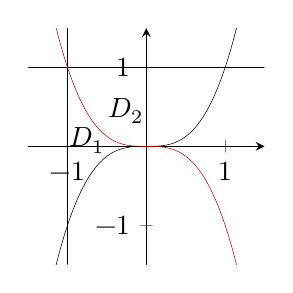
\begin{tikzpicture}[line cap=round,line join=round,x=1cm,y=1cm]
\begin{axis}[
x=1cm,y=1cm,
axis lines=middle,
xmin=-1.5,
xmax=1.5,
ymin=-1.5,
ymax=1.5,
xtick={-1,0,1},
ytick={-1,0,1},]
\draw [line width=0.2pt] (-1,-1.5) -- (-1,1.5);
\draw [line width=0.2pt,domain=-1.5:1.5] plot(\x,{(--1-0*\x)/1});
\draw[line width=0.2pt,smooth,samples=100,domain=-1.5:1.5] plot(\x,{(\x)^(3)});
\draw[line width=0.2pt,color=ccqqqq,smooth,samples=100,domain=-1.5:1.5] plot(\x,{0-(\x)^(3)});
\draw (-0.6,0.7360515021459239) node[anchor=north west] {$D_2$};
\draw (-1.1,0.36266094420600964) node[anchor=north west] {$D_1$};
\end{axis}
\end{tikzpicture}
\end{center}
\begin{align*}
I&=\iint_D=\iint_{D_1}+\iint_{D_2}\\
&=\iint_{D_1}[x+xyf(x^2+y^2)]dxdy+\iint_{D_2}x[1+yf(x^2+y^2)]dxdy\\
&=\iint_{D_1}xdxdy=2\int^0_{-1}dx\int^{-x^3}_0xdy\\
&=-\frac{2}{5}
\end{align*}
\end{examplle}

\begin{examplle}[]
设平面区域\(D=\{(x,y)\mid1\le x^2+y^2\le4,x\ge0,y\ge0\}\),计算
\begin{equation*}
\iint_D\frac{x\sin(\pi\sqrt{x^2+y^2})}{x+y}dxdy
\end{equation*}

由轮换对称性
\begin{align*}
&\iint_D\frac{x\sin(\pi\sqrt{x^2+y^2})}{x+y}dxdy\\
&=\frac{1}{2}\left[
\iint_D\frac{x\sin(\pi\sqrt{x^2+y^2})}{x+y}dxdy+
\iint_D\frac{y\sin(\pi\sqrt{x^2+y^2})}{x+y}dxdy
\right]\\
&=\frac{1}{2}\iint_D\sin(\pi\sqrt{x^2+y^2})dxdy=
\frac{1}{2}\int_0^{\frac{\pi}{2}}d\theta\int_1^2r\sin\pi rdr\\
&=-\frac{3}{4}
\end{align*}
\end{examplle}


\begin{examplle}[]
计算二重积分\(\iint_D\abs{x^2+y^2-1}d\sigma\),其中\(D=\{(x,y)\mid0\le
   x\le1,0\le y\le1\}\)

记\(D_1=\{(x,y)\mid x^2+y^2\le1,(x,y)\in D\},D_2=\{(x,y)\mid
   x^2+y^2>1,(x,y)\in D\}\),则

\begin{align*}
\iint_D\abs{x^2+y^2-1}d\sigma&=
-\iint_{D_1}(x^2+y^2-1)dxdy+\iint_{D_2}(x^2+y^2-1)dxdy\\
&=-2\iint_{D_1}(x^2+y^2-1)dxdy+\iint_D(x^2+y^2-1)dxdy
\end{align*}
\end{examplle}

\begin{examplle}[]
设\(f(x)\)为连续函数,\(F(t)=\int_1^tdy\int_y^tf(x)dx\),求\(F'(2)\)

交换积分次序得
\begin{equation*}
F(t)=\int_1^tdy\int_y^tf(x)dx=\int_1^t[\int_1^xf(x)dy]dx=\int_1^tf(x)(x-1)dx
\end{equation*}
因此\(F'(2)=f(2)(x-1)=f(2)\)
\end{examplle}

\begin{examplle}[]
计算二重积分\(\iint_Dr^2\sin\theta\sqrt{1-r^2\cos2\theta}drd\theta\),其中
\(D=\{(r,\theta)\mid 0\le r\le\sec\theta,0\le\theta\le\frac{\pi}{4}\}\)

直角坐标系下\(D=\{(x,y)\mid0\le x\le1,0\le y\le x\}\)
\end{examplle}

\begin{examplle}[]
已知函数\(f(x,y)\)具有二阶连续偏导数,且\(f(1,y)=0,f(x,1)=0\),
\(\iint_Df(x,y)dxdy=a\),其中\(D=\{(x,y)\mid0\le x\le1,0\le y\le1\}\),计算二
重积分
\begin{equation*}
\iint_Dxyf''_{xy}(x,y)dxdy
\end{equation*}

\begin{gather*}
\iint_Dxyf''_{xy}(x,y)dxdy=\int_0^1x(\int_0^1yf''_{xy}(x,y)dy)dx=\int_0^1x
(\int_0^1ydf_x'(x,y))dx\\
\int_0^1ydf_x'(x,y)=yf_x'(x,y)\Big\rvert_0^1-\int_0^1f'_x(x,y)dy=
-\int_0^1f_x'(x,y)dy\\
\int_0^1x(\int_0^1ydf_x'(x,y))dx=-\int_0^1x(\int_0^1f_x'(x,y)dy)dx=
-\int_0^1(\int_0^1xf_x'(x,y)dx)dy\\
\int_0^1xf_x'(x,y)dx=\int_0^1xdf(x,y)=xf(x,y)\Big\rvert_0^1-\int_0^1f(x,y)dx=
-\int_0^1f(x,y)dx\\
\iint_Dxyf''_{xy}dxdy=\int_0^1dy\int_0^1f(x,y)dx=a
\end{gather*}
\end{examplle}

\begin{examplle}[]
求积分\(\int_0^1dy\int_y^1\left(\frac{e^{x^2}}{x}-e^{y^2}\right)dx\)

\begin{align*}
\int_0^1dy\int_y^1\left(\frac{e^{x^2}}{x}-e^{y^2}\right)dx&=
\int_0^1dxf_0^x\left(\frac{e^{x^2}}{x}-e^{y^2}\right)dy=
\int_0^1(e^{x^2}-\int_0^xe^{y^2}dy)dx\\
&=\int_0^1e^{x^2}dx-\int_0^1(\int_0^xe^{y^2}dy)dx\\&=
\int_0^1e^{x^2}dx-x\int_0^xe^{y^2}dy\Big\rvert_0^1+
\int_0^1e^{x^2}\cdot xdx\\
&=\int_0^1e^{x^2}dx-\int_0^1e^{y^2}dy+\frac{1}{2}e^{x^2}\Big\rvert_0^1\\
&=\frac{e-1}{2}
\end{align*}
\end{examplle}

\begin{examplle}[]
设\(f(x)\)在\([a,b]\)上连续,且\(f(x)>0\),证明
\begin{equation*}
\int_a^bf(x)dx\int_a^b\frac{1}{f(x)}dx\ge(b-a)^2
\end{equation*}

令\(D=\{(x,y)\mid a\le x,y\le b\}\)
\begin{align*}
\int_a^bf(x)dx\int_a^b\frac{1}{f(x)}dx\ge(b-a)^2&=
\int_a^bf(x)dx\int_a^b\frac{1}{f(y)}dy\\
&=\iint_D\frac{f(x)}{f(y)}dxdy=\iint_D\frac{f(y)}{f(x)}dxdy\\
&=\frac{1}{2}\iint_D\left[\frac{f(x)}{f(y)}+\frac{f(y)}{f(x)}\right]dxdy\\
&\ge\iint_Ddxdy=(b-a)^2
\end{align*}
\end{examplle}

\begin{examplle}[]
证明
\(\left(\int_0^1e^{-x^2}dx\right)^2>\frac{\pi}{4}(1-\frac{1}{e})\)

令\(D=\{(x,y)\mid0\le x,y\le1\},D_1=\{(x,y)\mid x^2+y^2\le1,x\ge0,y\ge0\}\)
\begin{align*}
\left(\int_0^1e^{-x^2}dx\right)^2&=
\int_0^1e^{-x^2}dx\int_0^1e^{-y^2}dy=\iint_De^{-x^2-y^2}dxdy\\
&>\iint_De^{-(x^2+y^2)}dxdy=\int_0^{\frac{\pi}{2}}d\theta\int_0^1e^{-r^2}rdr=\frac{\pi}{4}(1-\frac{1}{e})
\end{align*}
\end{examplle}

\begin{examplle}[]
设函数\(z=f(x,y)\)具有二阶连续偏导数,且满足\(f_{xx}''=f_{yy}''\),又由
\(f(x,2x)=x\),\(f_x'(x,2x)=x^2\),试求二阶偏导数
\(f_{xx}''(x,2x),f_{xy}''(x,2x)\)

因为\(f_x'\cdot1+f_y'\cdot2=1\)所以\(2f_y'=1-x^2\)。又因为
\(2(f_{yx}''\cdot1+f_{yy}''\cdot2) =-2x\),由条件知\(f_x'(x,2x)=x^2\),则
\(f_{xx}''\cdot1+f_{xy}''\cdot2=2x\),解得
\(f_{xx}''(x,2x)=-\frac{4}{3}x,f_{xy}''(x,2x)=\frac{5}{3}x\)
\end{examplle}

\begin{examplle}[]
设函数\(u=u(x,y)\)由方程\(u=f(x,y,z,t),g(y,z,t)=0,h(z,t)=0\)所确定,求
\(\frac{\partial u}{\partial x},\frac{\partial u}{\partial y}\)

由方程组
\begin{equation*}
\begin{cases}
f(x,y,z,t)-u=0\\
g(y,z,t)=0\\
h(z,t)=0
\end{cases}
\end{equation*}
有
\begin{equation*}
\begin{cases}
\frac{\partial f}{\partial y}+\frac{\partial f}{\partial z}\frac{\partial z}{\partial y}+\frac{\partial f}{\partial t}\frac{\partial t}{\partial y}-\frac{\partial u}{\partial y}=0\\
\frac{\partial g}{\partial y}+\frac{\partial g}{\partial z}\frac{\partial z}{\partial y}+\frac{\partial g}{\partial t}\frac{\partial t}{\partial y}=0\\
\frac{\partial h}{\partial z}\frac{\partial z}{\partial y}+\frac{\partial h}{\partial t}\frac{\partial t}{\partial y}=0
\end{cases}
\end{equation*}
解
\end{examplle}
\subsection{无穷级数}
\label{sec:orgd9a0c8d}
\begin{examplle}[]
判断级数
\(\displaystyle\sum_{n=1}^\infty\int_0^{\frac{1}{n}}\frac{\sqrt{x}}{1+x^2}dx\)
的敛散性

由于
\begin{equation*}
0<\sum_{n=1}^\infty\int_0^{\frac{1}{n}}\frac{\sqrt{x}}{1+x^2}dx<
\int_0^{\frac{1}{n}}\sqrt{x}dx=\frac{2}{3}\frac{1}{n^{3/2}}
\end{equation*}
而级数\(\displaystyle\sum_{n=1}^\infty\frac{1}{n^{3/2}}\)收敛,因此级数收敛
\end{examplle}

\begin{examplle}[]
判断级数
\(\displaystyle\sum_{n=1}^\infty\left(\frac{1}{n}-\ln\frac{n+1}{n}\right)\)的
收敛性

由泰勒公式
\(\ln\frac{n+1}{n}=\frac{1}{n}-\frac{1}{2}\frac{1}{n^2}+o(\frac{1}{n^2})\),
则 \(\frac{1}{n}-\ln\frac{n+1}{n}\sim\frac{1}{2}\cdot\frac{1}{n^2}\),而
\(\displaystyle\sum_{n=1}^n\frac{1}{n^2}\)收敛
\end{examplle}

\begin{examplle}[]
判定级数\(\displaystyle\sum_{n=1}^\infty\sin(n\pi+\frac{1}{n-\ln n})\)的敛散
性

\(\displaystyle\sum_{n=1}^\infty\sin(n\pi+\frac{1}{n-\ln
   n})=\sum_{n=1}^\infty(-1)^n\sin\frac{1}{n-\ln n}\),令\(f(x)=\frac{1}{x-\ln
   x}\),则\(f'(x)<0\)且\(\lim_{n\to\infty}u_n=0\)
\end{examplle}

\begin{examplle}[]
判定级数\(\displaystyle\sum_{n=1}^\infty\frac{(-1)^n}{\sqrt{n}+(-1)^n}\)的敛
散性

\begin{equation*}
\frac{(-1)^n}{\sqrt{n}+(-1)^n}=
\frac{(-1)^n[\sqrt{n}-(-1)^n]}{n-1}=
\frac{(-1)^n\sqrt{n}}{n-1}-\frac{1}{n-1}
\end{equation*}
\end{examplle}

\begin{examplle}[]
\(\displaystyle\sum_{n=1}^{\infty}\left(\frac{\sin
   n\alpha}{n^2}-\frac{1}{\sqrt{n}}\right)\)

\(\displaystyle\sum_{n=1}^{\infty}\frac{\sin
   n\alpha}{n^2}\)收敛,\(\displaystyle\frac{1}{\sqrt{n}}\)发散,因此发散
\end{examplle}

\begin{examplle}[]
设\(\displaystyle
   a_1=2,a_{n+1}=\frac{1}{n}\left(a_n+\frac{1}{a_n}\right),n=1,2,\dots\),证明
\begin{enumerate}
\item \(\lim a_n\)存在
\item 级数\(\displaystyle\sum_{n=1}^\infty(\frac{a_n}{a_{n+1}}-1)\)收敛
\end{enumerate}


\begin{enumerate}
\item 显然\(a_n\ge0\),\(\{a_n\}\)单调减少且有下界,因此\(\lim a_n\)存在
\item 由于数列单调减少,所以有
\(\displaystyle
       0\le\frac{a_n}{a_{n+1}}-1=\frac{a_n-a_{n+1}}{a_{n+1}}\le a_n-a_{n+1}\),
而\(\displaystyle\sum_{n=1}^\infty(a_n-a_{n+1})=a_1-\lim_{n\to\infty}a_n\)
收敛
\end{enumerate}
\end{examplle}

\begin{examplle}[]
设正项数列\(\{a_n\}\)单调减少,且\(\displaystyle\sum_{n=1}^\infty(-1)^na_n\)
发散,试问级数
\(\displaystyle\sum_{n=1}^\infty\left(\frac{1}{a_n+1}\right)^n\)是否收敛
\end{examplle}

\begin{proof}
由已知正项数列\(\{a_n\}\)单调减少,根据单调有界数列必有极限知,极限
\(\lim_{n\to\infty}a_n\)存在,记\(a=\lim_{n\to\infty}a_n\),则有\(a_n\ge
   a\ge0\),若\(a=0\),则交错级数收敛,矛盾,因此\(a>0\)

又由于\(\left(\frac{1}{a_n+1}\right)^n\le\left(\frac{1}{a+1}\right)^n\),而
\(\frac{1}{a+1}<1\),几何级数\(\sum_{n=1}^\infty(\frac{1}{a+1})^n\)收敛,因此
级数收敛
\end{proof}

\begin{examplle}[]
求下列数列的极限
\begin{enumerate}
\item \(\displaystyle\lim_{n\to\infty}\frac{n!}{n^n}\)
\item \(\displaystyle\lim_{n\to\infty}\frac{n^n}{(n!)^2}\)
\end{enumerate}


\begin{enumerate}
\item 考虑级数\(\displaystyle\sum_{n=1}^\infty u_n=\sum_{n=1}^n\frac{n!}{n^n}\),
由于
\begin{equation*}
\lim_{n\to\infty}\frac{u_{n+1}}{u_n}=\lim_{n\to\infty}\frac{n^n}{(n+1)^n}=
\lim_{n\to\infty}\frac{1}{(1+\frac{1}{n})^n}=\frac{1}{e}<1
\end{equation*}
因此级数收敛,因此\(\displaystyle\lim_{n\to\infty}\frac{n!}{n^n}=0\)
\end{enumerate}
\end{examplle}

\begin{examplle}[]
求幂级数\(\displaystyle\sum_{n=1}^\infty(-1)^n\frac{n}{2^n}(x-1)^{2n}\)的收敛
域

令\(t=(x-1)^n\),考虑幂级数\(\displaystyle\sum_{n=1}^\infty(-1)^n\frac{n}{2^n}t^n\)
\end{examplle}

\begin{examplle}[]
设\(\displaystyle\sum_{n=1}^\infty\frac{(x-a)^n}{n}\)在\(x=-2\)处条件收敛,则
\(\displaystyle\sum_{n=1}^\infty n^2(x-a)^n\)在\(x=\ln\frac{1}{2}\)处
\begin{enumerate}
\item 绝对收敛
\item 条件收敛
\item 必发散
\item 敛散性由\(a\)决定
\end{enumerate}


幂级数\(\displaystyle\sum_{n=1}^\infty\frac{(x-a)^n}{n}\)的收敛半径是 1,因此
\(x=-2\)是收敛区间的端点,因此\(a=-3\)或-1,而\(a=-3\)与条件收敛矛盾,因此\(a=-1\)
\end{examplle}

\begin{examplle}[]
求幂级数\(\displaystyle\sum_{n=1}^\infty\frac{4n^2+4n+3}{2n+1}x^{2n}\)的收敛
域及和函数

\begin{equation*}
\sum_{n=1}^\infty\frac{4n^2+4n+3}{2n+1}x^{2n}=
\sum_{n=0}^\infty(2n+1)x^{2n}+\sum_{n=0}^\infty\frac{2}{2n+1}x^{2n}
\end{equation*}
因为
\begin{equation*}
\sum_{n=0}^\infty(2n+1)x^{2n}=\left(\sum_{n=0}^\infty x^{2n+1}\right)'=
\frac{1+x^2}{(1-x^2)^2},-1<x<1
\end{equation*}
当\(x\neq0\)时
\begin{gather*}
\sum_{n=0}^\infty\frac{2}{2n+1}x^{2n}=
\frac{2}{x}\sum_{x=0}^\infty\frac{1}{2n+1}x^{2n+1}\\
\left(\sum_{x=0}^\infty\frac{1}{2n+1}x^{2n+1}\right)'=
\sum_{n=0}^\infty x^{2n}=\frac{1}{1-x^2}\\
\sum_{x=0}^\infty\frac{1}{2n+1}x^{2n+1}=
\int_0^t\frac{1}{1-t^2}dt=\frac{1}{2}\ln\frac{1+x}{1-x},\quad -1<x<1
\end{gather*}
当\(x=0\)时,\(\displaystyle\sum_{n=0}^\infty\frac{2}{2n+1}x^{2n}=2\),所以
\begin{equation*}
\sum_{n=0}^\infty\frac{2}{2n+1}x^{2n}=
\begin{cases}
\frac{1}{x}\ln\frac{1+x}{1-x}&x\in(-1,0)\cup(0,1)\\
2&x=0
\end{cases}
\end{equation*}
当\(x=\pm1\)时,原级数发散

当\(x=0\)时,\(\displaystyle\sum_{n=1}^\infty\frac{4n^2+4n+3}{2n+1}x^{2n}=3\)

因此收敛区间与收敛域均为\(-1<x<1\),和函数
\begin{equation*}
S(x)=
\begin{cases}
\frac{1+x^2}{(1-x^2)^2}+\frac{1}{x}\ln\frac{1+x}{1-x}&x\in(-1,0)\cup(0,1)\\
3&x=0
\end{cases}
\end{equation*}
\end{examplle}

\begin{examplle}[]
求幂级数\(\displaystyle \sum_{n=1}^\infty\frac{1}{n2^n}x^{n-1}\)的收敛区间与
收敛域,并求其和函数

\begin{equation*}
\rho=\lim_{n\to\infty}\frac{\abs{a_{n+1}}}{\abs{a_n}}=\lim_{n\to\infty}
\frac{n2^n}{(n+1)2^{n+1}}=\frac{1}{2}
\end{equation*}
因此收敛半径为 2,收敛域为\([-2,2)\)

\begin{equation*}
S(x)=\sum_{n=1}^\infty\frac{1}{n2^n}x^n=
-\sum_{n=1}^\infty\frac{1}{n}(-1)^{n-1}\left(-\frac{x}{2}\right)^n=
-\ln(1-\frac{x}{2}),-1\le\frac{x}{2}<1
\end{equation*}
于是
\begin{equation*}
\sum_{n=1}^\infty\frac{1}{n2^n}x^{n-1}=
\begin{cases}
-\frac{1}{x}\ln\left(1-\frac{x}{2}\right)&x\in[-2,0)\cup(0,2)\\
\frac{1}{2}&x=0
\end{cases}
\end{equation*}
\end{examplle}

\begin{examplle}[]
设\(\{a_n\}\)满足条件:\(a_0=3,a_1=1,a_{n-2}-n(n-1)a_n=0(n\ge2)\),\(S(x)\)是
幂级数\(\displaystyle \sum_{n=0}^\infty a_nx^n\)的和函数
\begin{enumerate}
\item 证明\(S''(x)-S(x)=0\)
\item 求\(S(x)\)的表达式
\end{enumerate}


二阶常系数齐次线性微分方程\(S''(x)-S(x)=0\)的特征方程\(\lambda^2-1=0\)解得
\(\lambda=\pm1\),于是通解为
\begin{equation*}
S(x)=C_1e^x+C_2e^{-x}
\end{equation*}
代入得\(S(x)=2e^x+e^{-x}\)
\end{examplle}

\begin{examplle}[]
设\(a_0=1,a_1=1\),\(\displaystyle
   a_{n+1}=\frac{1}{n+1}(na_n+a_{n-1})(n=1,2,3,\dots)\),\(S(x)\)为幂级数
\(\displaystyle \sum_{n=0}^\infty a_nx^n\)的和函数
\begin{enumerate}
\item 证明幂级数的收敛半径不小于 1
\item 证明\((1-x)S'(x)-xS(x)=0(x\in(-1,1))\),并求\(S(x)\)的表达式
\end{enumerate}


\begin{enumerate}
\item 利用数学归纳法,\(0\le a_n\le1\),记\(R\)为幂级数的收敛半径,因为
\(\abs{a_nx^n}\le\abs{x}^n\),且级数\(\sum_0^\infty x^n\)绝对收敛,收敛半
径为\((-1,1)\),因此\((-1,1)\subseteq(-R,R)\)
\end{enumerate}
\end{examplle}

\begin{examplle}[]
求数项级数\(\displaystyle\sum_{n=0}^\infty\frac{n+1}{n!}\)的和

\begin{equation*}
\sum_{n=0}^\infty\frac{n+1}{n!}=
\sum_{n=0}^\infty\frac{n}{n!}+\sum_{n=0}^\infty\frac{1}{n!}=2e
\end{equation*}
\end{examplle}

\begin{examplle}[]
求级数\(\displaystyle \sum_{n=0}^\infty(-1)^n\frac{n^2-n+1}{2^n}\)

令\(S(x)=\displaystyle \sum_{n=2}^\infty n(n-1)x^{n-2}\),因此
\(S(x)=\left(\sum_{n=1}^\infty x^n\right)''=\left(\frac{x}{1-x}\right)''=\frac{2}{(1-x)^3}\)
\end{examplle}

\begin{examplle}[]
将\(f(x)=\arctan\displaystyle\frac{1+x}{1-x}\)展开为\(x\)的幂级数

因为\(f'(x)=\displaystyle\frac{1}{1+x^2}=\displaystyle
   \sum_{n=0}^\infty(-1)^nx^{2n}(-1<x<1)\),有
\begin{align*}
f(x)&=f(0)+\int_0^xf'(t)dt=\frac{\pi}{4}+\int_0^x \sum_{n=0}^\infty(-1)^nx^{2x}dx\\
&=\frac{\pi}{4}+ \sum_{n=0}^\infty\frac{(-1)^n}{2n+1}x^{2n+1}(-1\le x<1)
\end{align*}
\end{examplle}

\begin{examplle}[]
已知\(\displaystyle\cos2x-\frac{1}{(1+x)^2}=\displaystyle \sum_{n=0}^\infty
   a_nx^n(-1<x<1)\),求\(a_n\)

\begin{gather*}
\frac{1}{1+x}=\sum_{n=0}^\infty(-1)^nx^n,-1<x<1\\
\cos x=\sum_{n=0}^\infty(-1)^n\frac{x^{2n}}{(2n!)},-\infty<x<+\infty\\
-\frac{1}{(1+x)^2}=\left(\frac{1}{1+x}\right)'=\sum_{n=0}^\infty(-1)^{n+1}(n+1)x^n,-1<x<1
\end{gather*}
\end{examplle}

\begin{examplle}[]
设\(u_n=\displaystyle(-1)^n\ln\left(1+\frac{1}{\sqrt{n}}\right)\),则下列结论
成立的是
\begin{enumerate}
\item \(\displaystyle \sum_{n=1}^\infty u_n\)与
\(\displaystyle \sum_{n=1}^\infty u_n^2\)都收敛
\item \(\displaystyle \sum_{n=1}^\infty u_n\)与
\(\displaystyle \sum_{n=1}^\infty u_n^2\)都发散
\item \(\displaystyle \sum_{n=1}^\infty u_n\)收敛,
\(\displaystyle \sum_{n=1}^\infty u_n^2\)发散
\item \(\displaystyle \sum_{n=1}^\infty u_n\)发散,
\(\displaystyle \sum_{n=1}^\infty u_n^2\)收敛
\end{enumerate}


\(\ln^2(1+\frac{1}{\sqrt{n}})\sim\frac{1}{n}\)
\end{examplle}

\begin{examplle}[]
设\(\displaystyle \sum_{n=1}^\infty u_n^2\)收敛,则
\(\abs{\u_n}{n}\le\frac{1}{2}(u_n^2+\frac{1}{n^2})\),因此 \(\displaystyle
   \sum_{n=1}^\infty\frac{u_n}{n}\)收敛
\end{examplle}

\begin{examplle}[]
设\(\{a_n\}\)是单调增加且有界的正数列,证明级数\(\displaystyle
   \sum_{n=1}^\infty\left(1-\frac{a_n}{a_{n+1}}\right)\)收敛

\begin{equation*}
1-\frac{a_n}{a_{n+1}}\le\frac{1}{a_1}(a_{n+1}-a_n)
\end{equation*}
\end{examplle}

\begin{examplle}[]
求级数\(\displaystyle\sum_{n=1}^\infty\frac{(-1)^{n-1}}{(2n-1)(2n+1)}\)

令\(f(x)=\displaystyle\sum_{n=1}^\infty\frac{(-1)^{n-1}}{(2n-1)(2n+1)}x^{2n+1}\)
\end{examplle}


\subsection{常微分方程与差分方程}
\label{sec:org0012aa0}
\begin{examplle}[]
求解下列初值问题
\begin{equation*}
(x+y)dx+(y-x)dy=0,y|_{x=1}=-1
\end{equation*}

\begin{equation*}
\frac{dy}{dx}=\frac{x+y}{x-y}
\end{equation*}
令\(u=\frac{y}{x}\),分离变量得
\begin{gather*}
\frac{1-u}{1+u^2}du=\frac{dx}{x}\\
\abs{x}\sqrt{1+u^2}=Ce^{\arctan u}\\
\sqrt{x^2+y^2}=Ce^{\arctan\frac{y}{x}}\\
\sqrt{x^2+y^2}=\sqrt{2}e^{\arctan\frac{y}{x}+\frac{\pi}{4}}
\end{gather*}
\end{examplle}

\begin{examplle}[]
求\(\frac{dy}{dx}=\frac{1-y}{y-x}\)的通解

\begin{equation*}
\frac{dx}{dy}=\frac{y-x}{1-y}=-\frac{1}{1-y}x+\frac{y}{1-y}
\end{equation*}
求解通解
\begin{equation*}
x=(1-y)\ln\abs{1-y}+C(1-y)+1
\end{equation*}
\end{examplle}

\begin{remark}
形如\(\frac{dy}{dx}=\frac{s(y)}{t(y)x+q(y)}\)的微分方程,将\(x\)看作未知量
\end{remark}

\begin{examplle}[]
解微分方程
\(\displaystyle\frac{dy}{dx}=\frac{y-x+1}{y+x+5}\)

方程组
\begin{equation*}
\begin{cases}
y-x+1=0\\
y+x+5=0
\end{cases}
\end{equation*}
有唯一解\(x=-2,y=-3\),令\(u=x+2,v=y+3\),则\(\frac{dv}{du}=\frac{v-u}{v+u}\),
再令\(z=\frac{v}{u}\),有
\begin{equation*}
z+u\frac{dz}{du}=\frac{z-1}{z+1},-\frac{z+1}{z^2+1}dz=\frac{1}{u}du
\end{equation*}
因此
\begin{equation*}
-\frac{1}{2}\ln(z^2+1)-\arctan z=\ln\abs{u}+C
\end{equation*}
\end{examplle}

\begin{remark}
对方程\(\displaystyle\frac{dy}{dx}=f\left(\frac{a_1x+b_1y+C_1}{a_2x+b_2y+C_2}\right)\)
\begin{enumerate}
\item 若\(\displaystyle\frac{a_1}{a_2}=\frac{b_1}{b_2}=k\),则令\(z=a_2x+b_2y\),
方程化为
\begin{equation*}
\frac{dz}{dx}=b_2f\left(\frac{kz+C_1}{z+C_2}\right)+a_2
\end{equation*}
\item 若\(\displaystyle\frac{a_1}{a_2}=\frac{b_1}{b_2}=k\),则方程组
\begin{equation*}
\begin{cases}
a_1x+b_1y+C_1=0\\
a_2x+b_2y+C_2=0
\end{cases}
\end{equation*}
有唯一解\(x=\alpha,y=\beta\),令\(u=x-\alpha,v=y-\beta\),则
\begin{equation*}
\frac{dv}{du}=
f\left(
\frac{a_1+b_1\frac{v}{u}}{a_2+b_2\frac{v}{u}}\right)=
g\left(\frac{v}{u}\right),g(t)=f\left(\frac{a_1+b_1t}{a_2+b_2t}\right)
\end{equation*}
\end{enumerate}
\end{remark}

\begin{examplle}[]
求\(y''+y=\sin x+x\cos 2x\)的通解

特征方程的根为\(\lambda=\pm i\),\(y''+y=4\sin x\)的特解为\(y_1^*=-2x\cos x\),
\(y''+y=x\cos 2x\)特解为\(y_2^*=-\frac{1}{3}x\cos x +\frac{4}{9}\sin 2x\)
\end{examplle}
\section{线性代数}
\label{sec:orge0800d7}
\subsection{行列式}
\label{sec:org8903a97}
\begin{examplle}[]
计算行列式
\begin{equation*}
D_n=
\begin{vmatrix}
a_1&-1&0&\cdots&0&0\\
a_2&x&-1&\cdots&0&0\\
a_3&0&x&\cdots&0&0\\
\vdots&\vdots&\vdots&&\vdots&\vdots\\
a_{n-1}&0&0&\cdots&x&-1\\
a_n&0&0&\cdots&0&x
\end{vmatrix}
\end{equation*}

\begin{align*}
D_n&=
\begin{vmatrix}
a_1&-1&0&\cdots&0&0\\
a_2+a_1x&0&-1&\cdots&0&0\\
a_3&0&x&\cdots&0&0\\
\vdots&\vdots&\vdots&&\vdots&\vdots\\
a_{n-1}&0&0&\cdots&x&-1\\
a_n&0&0&\cdots&0&x
\end{vmatrix}\\
&=\cdots=
\begin{vmatrix}
a_1&-1&0&\cdots&0&0\\
a_2+a_1x&0&-1&\cdots&0&0\\
a_3+a_2x+a_1x^2&0&0&\cdots&0&0\\
\vdots&\vdots&\vdots&&\vdots&\vdots\\
a_{n-1}+\dots+a_1x^{n-2}&0&0&\cdots&0&-1\\
a_n+\dots+a_1x^{n-1}&0&0&\cdots&0&0
\end{vmatrix}\\
&=a_1x^{n-1}+\dots+a_n
\end{align*}
\end{examplle}

\begin{examplle}[]
计算
\begin{equation*}
\begin{vmatrix}
a&b&c&d\\x&0&0&y\\
y&0&0&x\\d&c&b&a
\end{vmatrix}
\end{equation*}

\begin{equation*}
\begin{vmatrix}
a&b&c&d\\x&0&0&y\\
y&0&0&x\\d&c&b&a
\end{vmatrix}=-
\begin{vmatrix}
y&0&0&x\\x&0&0&y\\a&b&c&d\\d&c&b&a
\end{vmatrix}=
\begin{vmatrix}
y&x&0&0\\x&y&0&0\\
a&d&c&b\\d&a&b&c
\end{vmatrix}=(x^2-y^2)(b^2-c^2)
\end{equation*}
\end{examplle}

\begin{examplle}[]
已知\(\bA,\bB\)均为\(n\)阶矩阵,若
\(\abs{\bA}=3,\abs{\bB}=2,\abs{\bA^{-1}+\bB}=2\),求
\(\abs{\bA+\bB^{-1}}\)

\begin{align*}
\abs{\bA+\bB^{-1}}&=\abs{\bE\bA+\bB^{-1}\bE}=\abs{(\bB^{-1}\bB)\bA+\bB^{-1}(\bA^{-1}\bA)}\\
&=\abs{\bB^{-1}(\bB+\bA^{-1})\bA}=3
\end{align*}
\end{examplle}

\begin{examplle}[]
已知 4 阶矩阵\(\bA\)相似于\(\bB,\bA\)的特征值为 2,3,4,5,\(\bE\)为 4 阶单位矩阵,
求\(\abs{\bB-\bE}\)

\(\bA=T\bB T^{-1}=Q\bD Q^{-1}\),\(\abs{\bB-\bE}=\abs{TQ(\bD-\bE)Q^{-1}T^{-1}}=24\)
\end{examplle}

\begin{examplle}[]
满足\(\bA^T=-\bA\)的矩阵称为反对称矩阵,证明:若\(\bA\)是反对称矩阵,则
\(\abs{\bA}=0\)

设\(\bA\)的阶数为\(2k+1\),\(k\)为正整数,
\(\abs{\bA}=\abs{\bA^T}=\abs{-\bA}=(-1)^{2k+1}\abs{A}=-\abs{A}\),得\(\abs{\bA}=0\)
\end{examplle}

\begin{examplle}[]
已知\(\bA,\bB\)都是\(n\)阶非零矩阵,满足\(\bA\bB=\bzero\),证明
\(\abs{\bA}=0\)

若\(\abs{\bA}\neq0\),则\(\bA\)可逆,\(\bB=\bzero\),矛盾
\end{examplle}

\begin{examplle}[]
已知\(\xi\)是\(n\)维向量,且\(\xi^T\xi=1\),若\(\bA=\bE-\xi\xi^T\),证明
\(\abs{\bA}=0\)

\begin{equation*}
\bA\xi=(\bE-\xi\xi^T)\xi=\xi-\xi=\bzero
\end{equation*}
有特征值 0,从而齐次线性方程组\(\bA\bx=\bzero\)有非零解,因此\(\abs{\bA}=0\)
\end{examplle}


\begin{examplle}[]
已知
\begin{equation*}
\abs{\bA}=
\begin{vmatrix}
1&0&3\\-1&2&4\\1&5&9
\end{vmatrix}
\end{equation*}
\begin{enumerate}
\item 求\(A_{12}-A_{22}+A_{32}\)
\item 求\(A_{31}+A_{32}+A_{33}\)
\end{enumerate}


\begin{enumerate}
\item \(A_{12}-A_{22}+A_{32}=a_{11}A_{12}+a_{21}A_{22}+a_{31}A_{33}=0\)
\item 由于代数余子式\(A_{ij}\)的值与元素\(a_{ij}\)的值无关,可构造一个新的行列式
\begin{equation*}
\abs{\bB}=
\begin{vmatrix}
1&0&3\\-1&2&4\\1&1&1
\end{vmatrix}=-11
\end{equation*}
因此 \(A_{31}+A_{32}+A_{33}=-11\)
\end{enumerate}
\end{examplle}

\begin{examplle}[]
若
\begin{equation*}
\abs{\bA}=
\begin{vmatrix}
1&2&3&4&5\\
2&2&2&1&1\\
3&1&2&4&5\\
1&1&1&2&2\\
4&3&1&5&0
\end{vmatrix}
\end{equation*}
求\(A_{31}+A_{32}+A_{33}\)
由
\begin{equation*}
\abs{\bB_1}=
\begin{vmatrix}
1&2&3&4&5\\
2&2&2&1&1\\
2&2&2&1&1\\
1&1&1&2&2\\
4&3&1&5&0
\end{vmatrix}=0,\abs{\bB_2}=
\begin{vmatrix}
1&2&3&4&5\\
2&2&2&1&1\\
1&1&1&2&2\\
1&1&1&2&2\\
4&3&1&5&0
\end{vmatrix}=0
\end{equation*}
有
\begin{equation*}
\begin{cases}
2A_{31}+2A_{32}+2A_{33}+A_{34}+A_{35}=0\\
A_{31}+A_{32}+A_{33}+2A_{34}+2A_{35}=0
\end{cases}
\end{equation*}
因此\(A_{31}+A_{32}+A_{33}=0\)
\end{examplle}

\begin{examplle}[]
若
\begin{equation*}
\bA=
\begin{bmatrix}
1&2&0&0\\
3&5&0&0\\
0&0&4&-6\\
0&0&0&1
\end{bmatrix}
\end{equation*}
因 \(\abs{\bA}=-4\),
\begin{equation*}
\bA^{-1}=
\begin{bmatrix}
-5&2&0&0\\
3&-1&0&0\\
0&0&\frac{1}{4}&\frac{3}{2}\\
0&0&0&1
\end{bmatrix}
\end{equation*}
因此
\begin{equation*}
\bA^*=\abs{\bA}\bA^{-1}=
\begin{bmatrix}
20&-8&0&0\\
-12&4&0&0\\
0&0&-1&-6\\
0&0&0&-4
\end{bmatrix}
\end{equation*}
\end{examplle}
\subsection{矩阵}
\label{sec:org0d2099a}
\begin{examplle}[]
已知\(\bA,\bB\)都是\(n\)阶矩阵,且\(\bA\bB=\bA+\bB\),证明\(\bA\bB=\bB\bA\)

有
\begin{equation*}
\bA\bB-\bA-\bB+\bE=(\bA-\bE)(\bB-\bE)=\bE
\end{equation*}
因此\(\bA-\bE\)可逆,\((\bA-\bE)^{-1}=\bB-\bE\),于是
\begin{equation*}
(\bA-\bE)(\bB-\bE)=(\bB-\bE)(\bA-\bE)
\end{equation*}
\end{examplle}

\begin{examplle}[]
已知
\begin{equation*}
\bA=
\begin{bmatrix}
2&1&-1\\6&3&-3\\-4&-2&2
\end{bmatrix}
\end{equation*}
求\(\bA^n\)

\begin{equation*}
\bA=
\begin{bmatrix}
1\\3\\-2
\end{bmatrix}
\begin{bmatrix}
2&1&-1
\end{bmatrix}
\end{equation*}
那么
\begin{equation*}
\bA^2=
\begin{bmatrix}
1\\3\\-2
\end{bmatrix}\left(
\begin{bmatrix}
2&1&-1
\end{bmatrix}
\begin{bmatrix}
1\\3\\-2
\end{bmatrix}
\right)
\begin{bmatrix}
 2&1&-1
\end{bmatrix}=7\bA
\end{equation*}
\end{examplle}

\begin{remark}
一般情况下,若\(r(\bA)=1\),则\(\bA\)可分解为两个矩阵的乘积,有\(\bA^2=l\bA\),
从而
\begin{equation*}
\bA^n=l^{n-1}\bA
\end{equation*}
例如
\begin{equation*}
\bA=
\begin{bmatrix}
a_1b_1&a_1b_2&a_1b_3\\
a_2b_1&a_2b_2&a_2b_3\\
a_3b_1&a_3b_2&a_3b_3\\
\end{bmatrix}=
\begin{bmatrix}
a_1\\a_2\\a_3
\end{bmatrix}
\begin{bmatrix}
b_1&b_2&b_3
\end{bmatrix}=\balpha\bbeta^T
\end{equation*}
那么
\begin{equation*}
\bA^2=(\balpha\bbeta)^T(\balpha\bbeta^T)=\balpha(\bbeta^T\balpha)\bbeta^T=l\bA
\end{equation*}
\end{remark}


\begin{examplle}[]
设\(n\)阶矩阵\(\bA\)满足\(\bA^2+2\bA-3\bE=\bzero\)
\begin{enumerate}
\item 证明\(\bA,\bA+2\bE\)可逆
\item 当\(\bA\neq\bE\)时,判断\(\bA+3\bE\)是否可逆
\end{enumerate}


\begin{enumerate}
\item \((\bA+3\bE)(\bA-\bE)=\bzero\),因为\(\bA\neq\bE\),则
\((\bA+3\bE)\bx=\bzero\)有非零解,因此\(\abs{\bA+3\bE}=0\),所以
\(\bA+3\bE\)不可逆
\end{enumerate}
\end{examplle}

\begin{examplle}[]
设\(\bA,\bB\)为\(n\)阶矩阵,如果\(\bE+\bA\bB\)可逆,证明矩阵\(\bE+\bB\bA\)可
逆

如果\(\bE+\bB\bA\)不可逆,则\(\abs{\bE+\bB\bA}=0\),那么齐次方程组
\((\bE+\bB\bA)\bx=\bzero\)有非零解

设\(\boldeta\)是非零解,则
\((\bE+\bB\bA)\boldeta=\bzero\),\(\bB\bA\boldeta=-\boldeta\)。因为
\((\bE+\bA\bB)(\bA\boldeta)=\bA\boldeta+\bA(\bB\bA\boldeta)=\bzero\),且
\(\bA\boldeta\neq\bzero\),因此矛盾
\end{examplle}

\begin{examplle}[]
计算
\begin{equation*}
\begin{bmatrix}
1&0&0\\
0&1&0\\
0&2&1
\end{bmatrix}^{2000}
\begin{bmatrix}
1&2&3\\
2&3&4\\
3&4&5
\end{bmatrix}
\end{equation*}

\begin{equation*}
\begin{bmatrix}
1&0&0\\
0&1&0\\
0&2&1
\end{bmatrix}
\end{equation*}
是把第 2 行的 2 倍加到第 3 行
\end{examplle}

\begin{examplle}[]
已知\(a\)是常数,且矩阵
\begin{equation*}
\bA=
\begin{bmatrix}
1&2&a\\1&3&0\\2&7&-a
\end{bmatrix}
\end{equation*}
可经初等变换化为矩阵
\begin{equation*}
\bB=
\begin{bmatrix}
1&a&2\\0&1&1\\-1&1&1
\end{bmatrix}
\end{equation*}
\begin{enumerate}
\item 求\(a\)
\item 求满足\(\bA\bP=\bB\)的可逆矩阵
\end{enumerate}


\begin{equation*}
\abs{\bA}=
\begin{vmatrix}
1&2&a\\1&3&0\\2&7&-a
\end{vmatrix}=
\begin{vmatrix}
1&2&a\\1&3&0\\3&9&0
\end{vmatrix}=0
\end{equation*}
\(r(\bA)=2\),因此\(r(\bB)=2\),而\(\abs{\bB}=2-a\),因此\(a=2\)

\begin{equation*}
\begin{bNiceArray}{c|c}
A&B
\end{bNiceArray}=
\begin{bNiceArray}{ccc:ccc}
1&2&2&1&2&2\\
1&3&0&0&1&1\\
2&7&-2&-1&-1&-1
\end{bNiceArray}=
\begin{bNiceArray}{ccc:ccc}
1&0&6&3&4&4\\
0&1&-2&-1&-1&-1\\
0&0&0&0&0&0
\end{bNiceArray}
\end{equation*}
因此
\begin{equation*}
\bP=
\begin{bmatrix}
3-6k_1&4-6k_1&4-6k_3\\
-1+2k_1&-1+2k_2&-1+2k_3\\
k_1&k_2&k_3
\end{bmatrix}
\end{equation*}
\end{examplle}

\begin{examplle}[]
\begin{enumerate}
\item 已知
\begin{equation*}
\bA=
\begin{bmatrix}
1&2&5\\2&a&7\\1&3&2
\end{bmatrix},\bB=
\begin{bmatrix}
1&0&4\\0&2&-1\\-3&0&5
\end{bmatrix}
\end{equation*}
且\(r(\bA\bB)=2\),求\(a\)
\item 已知\(\bA\)是 2 阶非 0 矩阵且\(\bA^5=\bzero\),求\(r(\bA)\)
\end{enumerate}


\begin{enumerate}
\item \(\abs{\bB}\neq0\),因此\(r(\bA)=2,\abs{\bA}=0\),而
\(\abs{\bA}=3(5-a)=0\),因此\(a=5\)
\item \(r(\bA)\ge1\),\(\abs{\bA}^5=0\),因此\(\abs{\bA}=0\),因此\(r(\bA)=1\)
\end{enumerate}
\end{examplle}

\begin{examplle}[]
设\(\bA,\bB\)是 3 阶矩阵
\begin{enumerate}
\item 证明\(r(\bA,\bA\bB)=r(\bA)\)
\item 举例说明\(r(\bA,\bB\bA)=r(\bA)\)是错误的
\end{enumerate}


\begin{enumerate}
\item 设\(\bA\bB=\bC\),对矩阵\(\bA,\bC\)分别按列分块,记
\(\bA=[\balpha_1,\balpha_2,\balpha_3],
      \bC=[\bgamma_1,\bgamma_2,\bgamma_3]\),记\(\bB=[b_{ij}]\),那么由
\(\bA\bB=\bC\),有
\begin{equation*}
\begin{bmatrix}
\balpha_1&\balpha_2&\balpha_3
\end{bmatrix}
\begin{bmatrix}
b_{11}&b_{12}&b_{13}\\
b_{21}&b_{22}&b_{23}\\
b_{31}&b_{32}&b_{33}\\
\end{bmatrix}=
\begin{bmatrix}
\bgamma_1&\bgamma_2&\bgamma_3
\end{bmatrix}
\end{equation*}
即
\begin{equation*}
\begin{cases}
\bgamma_1=b_{11}\balpha_1+b_{21}\balpha_2+b_{31}\balpha_3\\
\bgamma_2=b_{12}\balpha_2+b_{22}\balpha_2+b_{32}\balpha_3\\
\bgamma_3=b_{13}\balpha_3+b_{23}\balpha_2+b_{33}\balpha_3\\
\end{cases}
\end{equation*}
因此\(\bgamma_1,\bgamma_2,\bgamma_3\)可由\(\balpha_1,\balpha_2,\balpha_3\)
线性表示,因此
\begin{equation*}
r(\bA,\bA\bB)=r(\balpha_1,\balpha_2,\balpha_3,\bgamma_1,\bgamma_2,\bgamma_3)=
r(\balpha_1,\balpha_2,\balpha_3)=r(\bA)
\end{equation*}
\item \begin{equation*}
\bA=
\begin{bmatrix}
1&0&0\\0&0&1\\0&0&0
\end{bmatrix},\bB=
\begin{bmatrix}
1&0&0\\0&0&1\\0&1&0
\end{bmatrix}
\end{equation*}
\end{enumerate}
\end{examplle}

\begin{examplle}[]
设\(\bA\)是\(m\times n\)矩阵,\(\bB\)是\(n\times s\)矩阵,证明
\begin{equation*}
r(\bA\bB)\le\min\{r(\bA),r(\bB)\}
\end{equation*}

对于齐次方程组 1. \(\bA\bB\bx=\bzero\)2. \(\bB\bx=\bzero\),若\(\balpha\)是方
程组 2 的一个解,它也是方程组 1 的解,因此方程组 2 的解集是方程组 1 的解集的
子集

又因 1 的解向量的秩为\(s-r(\bA\bB)\),2的解向量的秩为\(s-r(\bB)\),因此
\begin{equation*}
s-r(\bB)\le s-r(\bA\bB)
\end{equation*}
即\(r(\bA\bB)\le r(\bB)\)

另一方面,\(r(\bA\bB)=r((\bA\bB)^T)=r(\bB^T\bA^T)\le r(\bA^T)=r(\bA)\)
\end{examplle}

\begin{examplle}[]
若\(\bA\)为\(n\)阶矩阵,且\(\bA^2=\bE\),证明
\begin{equation*}
r(\bA+\bE)+r(\bA-\bE)=n
\end{equation*}

\(r(\bA+\bE)+r(\bA-\bE)\le n+r((\bA-\bE)(\bA+\bE))\).
\(r(\bA+\bE)+r(\bA-\bE)\ge r(\bA+\bE+\bE-\bA)\)
\end{examplle}

\begin{examplle}[]
已知\(\balpha_1,\dots,\balpha_n\)线性无关,证明
\(\balpha_1-\balpha_2,\balpha_2-\balpha_3,\dots,\balpha_n-\balpha_1\)线性相关

令

\begin{gather*}
\bA=
\begin{bmatrix}
1&0&\dots&0&-1\\
-1&0&\dots&0&0\\
\vdots&\vdots&&\vdots&\vdots\\
0&0&\dots&1&0\\
0&0&\dots&-1&1
\end{bmatrix}\\
\begin{bmatrix}
\balpha_1-\balpha_2&\balpha_2-\balpha_3&\dots&\balpha_n-\balpha_1
\end{bmatrix}=
\begin{bmatrix}
\balpha_1&\dots&\balpha_n
\end{bmatrix}
\bA
\end{gather*}
\(\abs{\bA}=0\),因此线性相关
\end{examplle}

\begin{examplle}[]
设\(\bA\)是\(n\times m\)矩阵,\(\bB\)是\(m\times n\)矩阵,其中\(n<m\),若
\(\bA\bB=\bE\),证明\(\bB\)的列向量线性无关

\(r(\bB)\le n\),又
\begin{equation*}
r(\bB)\ge r(\bA\bB)=n
\end{equation*}
\end{examplle}

\begin{examplle}[]
设\(\balpha_i=[a_{i1},\dots,a_{in}]^T(i=1,2,\dots,r,r<n)\)是\(n\)维实向量,且
\(\balpha_1,\dots,\balpha_r\) 线性无关,已知\(\bbeta=[b_1,\dots,b_n]^T\)是线
性方程组
\begin{equation*}
\begin{cases}
a_{11}x_1+\dots+a_{1n}x_n=0\\
\dots\\
a_{r1}x_1+\dots+a_{rn}x_n=0\\
\end{cases}
\end{equation*}
的非零解向量,试判断向量组\(\balpha_1,\dots,\balpha_r,\bbeta\)的线性相关性

设\(k_1\balpha_1+\dots+k_r\balpha_r+k\bbeta=\bzero\).
\(\bbeta\)与每个\(\balpha_i\)都正交,\(\bbeta^T\balpha_i=0\)。因此
\(k\bbeta^T\bbeta=0\).因为\(\bbeta\neq\bzero\),因此\(\bbeta^T\bbeta\neq0\),
因此\(k=0\).因此线性无关
\end{examplle}

\begin{examplle}[]
设\(n\)维列向量\(\balpha_1,\dots,\balpha_{n-1}\)线性无关,且与非零向量
\(\bbeta_1,\bbeta_2\)正交,证明\(\bbeta_1,\bbeta_2\)线性相关

令
\begin{equation*}
\bA=
\begin{bmatrix}
\balpha_1^T\\\vdots\\\balpha_{n-1}^T
\end{bmatrix}
\end{equation*}
因此\(\bA\bbeta_1=\bA\bbeta_2=\bzero\),因为\(r(\bA)=n-1\),因此
\(\bA\bx=\bzero\)的基础解系仅由 1 个解向量构成,因此\(\bbeta_1,\bbeta_2\)线性相
关
\end{examplle}

\begin{examplle}[]
线性变换\(\bA\)的属于不同特征值的特征向量线性无关

设\(\bA\)的\(k\)个不同特征值\(\lambda_1,\dots,\lambda_k\)分别对应于特征向量
\(\xi_1,\dots,\xi_k\),对\(k\)作数学归纳法

当\(k=1\)时显然。设命题在\(k-1\)个不同特征值的情况下成立
\begin{gather*}
l_1\xi_1+\dots+l_k\xi_k=0\\
l_1\bA\xi_1+\dots+l_k\bA\xi_k=0\\
l_1\lambda_1\xi_1+\dots+l_k\lambda_k\xi_k=0\\
l_2(\lambda_1-\lambda_2)\xi_2+\dots+l_k(\lambda_1-\lambda_k)\xi_k=0\\
l_2(\lambda_1-\lambda_2)=\cdots=l_k(\lambda_1-\lambda_k)=0\\
l_2=\dots=l_k=0
\end{gather*}
因此\(l_1=0\),\(\xi_1,\dots,\xi_k\)线性无关
\end{examplle}

\begin{examplle}[]
设\(\bA,\bB\)都是\(m\times n\)矩阵,证明\(r(\bA+\bB)\le r(\bA)+r(\bB)\)

设\(r(\bA)=r\),\(\balpha_{i_1},\dots,\balpha_{i_r}\)是\(\bA\)的列向量的极大线
性无关组,\(r(\bB)=t\),\(\bbeta_{j_1},\dots,\bbeta_{j_t}\)是\(\bB\)的列向量的
极大线性无关组

于是\(\balpha_k+\bbeta_k\)都被
\(\balpha_{i_1},\dots,\balpha_{i_r},\bbeta_{j_1},\bbeta_{j_t}\)线性表示
\end{examplle}

\begin{examplle}[]
已知向量组
\begin{align*}
&\balpha_1=(1,1,4)^T,\balpha_2=(1,0,4),\balpha_3=(1,2,a^2+3)^T\\
&\bbeta_1=(1,1,a+3),\bbeta_2=(0,2,1-a),\bbeta_3=(1,3,a^2+3)^T
\end{align*}
若两向量组等价,求\(a\)的值,并将\(\bbeta_3\)用
\(\balpha_1,\balpha_2,\balpha_3\)线性表示

因为两个向量组等价,因此 
\(r(\balpha_1,\balpha_2,\balpha_3)=r(\balpha_1,\balpha_2,\balpha_3,
   \bbeta_1,\bbeta_2,\bbeta_3)=r(\bbeta_1,\bbeta_2,\bbeta_3)\)

\begin{align*}
[\balpha_1,\balpha_2,\balpha_3\mid\bbeta_1,\bbeta_2,\bbeta_3]&=
\begin{bNiceArray}{ccc:ccc}
1&1&1&1&0&1\\
1&0&2&1&2&3\\
4&4&a^2+3&a+3&1-a&a^2+3
\end{bNiceArray}\\
&\to\begin{bNiceArray}
1&1&1&1&0&1\\
0&-1&1&0&2&2\\
0&0&a^2-1&a-1&1-a&a^2-1
\end{bNiceArray}
 \end{align*}
\end{examplle}

\subsection{线性方程组}
\label{sec:org128db69}
\begin{examplle}[]
设非齐次线性方程组\(\bA_{m\times n}\bx=\bb\),则
\begin{enumerate}
\item 当\(r(\bA)=m\)时,方程有解
\item 当\(r(\bA)=n\)时,方程有唯一解
\item 当\(m=n\)时,方程组有唯一解
\item 当\(r(\bA)=r<n\)时,方程组有无穷多解
\end{enumerate}


\(\bA\bx=\bb\)有解当且仅当\(r(\bA)=r(\bA,\bb)\)
\end{examplle}

\begin{examplle}[]
设\(\bA\)是四阶矩阵,\(r(\bA)=2\),\(\boldeta_1,\boldeta_2,\boldeta_3\)是
\(\bA\bx=\bb\)的三个线性无关解,其中
\begin{align*}
&\boldeta_1+\boldeta_2=[-1,2,5,1]^T\\
&\boldeta_2-2\boldeta_3=[2,1,3,-3]^T\\
&3\boldeta_1+5\boldeta_2=[1,-2,1,-1]^T
\end{align*}
求方程组\(\bA\bx=\bb\)的通解

因为\(\bA(\boldeta_2-2\boldeta_3)=-\bb\),因此
\(\boldeta=-\boldeta_2+2\boldeta_3\)是\(\bA\bx=\bb\)的一个特解

\(\bA\bx=\bzero\)的两个通解为
\begin{align*}
&\bxi_1=\boldeta_1+\boldeta_2+2(\boldeta_2-2\boldeta_3)\\
&\bxi_2=8(\boldeta_2-2\boldeta_3)+5\boldeta_3+3\boldeta_1
\end{align*}
\end{examplle}

\begin{examplle}[]
设\(\bxi=[a_1,\dots,a_n]^T,\bxi^T\bxi=1\),证明\(\abs{\bE-\bxi^T\bxi}=0\)

构造齐次线性方程组
\begin{equation*}
(\bE-\bxi^T\bxi)\bx=\bzero
\end{equation*}
有
\begin{equation*}
(\bE-\bxi^T\bxi)\bxi=\bzero
\end{equation*}
有非零解,因此
\begin{equation*}
\abs{\bE-\bxi^T\bxi}\neq0
\end{equation*}
\end{examplle}


\begin{examplle}[]
设齐次线性方程组
\begin{equation*}
\begin{cases}
(1+a)x_1+2x_2+\dots+nx_n=0\\
x_1+(2+a)x_2+\dots+nx_n=0\\
\vdots\\
x_1+2x_2+\dots+(a_n+n)x_n=0
\end{cases}
\end{equation*}
试问\(a\)为何值时,方程组有非零解

\begin{equation*}
\bA=
\begin{bmatrix}
1+a&2&\dots&n\\
1&2+a&\dots&n\\
\vdots&\vdots&&\vdots\\
1&2&\dots&n+a
\end{bmatrix}\to
\begin{bmatrix}
1+a&2&\dots&n\\
-a&a&\dots&0\\
\vdots&\vdots&&\vdots\\
-a&0&\dots&a
\end{bmatrix}=\bB
\end{equation*}
当\(a=0\)时,\(r(\bA)=1<n\),方程组有非零解

当\(a\neq0\)时,对矩阵\(\bB\)继续初等行变换
\begin{align*}
\bB&\to
\begin{bmatrix}
1+a&2&\dots&n\\
-a&a&\dots&0\\
\vdots&\vdots&&\vdots\\
-a&0&\dots&a
\end{bmatrix}\to
\begin{bmatrix}
1+a&2&\dots&n\\
-1&1&\dots&0\\
\vdots&\vdots&&\vdots\\
-1&0&\dots&1
\end{bmatrix}\\
&\to
\begin{bmatrix}
\frac{n(n+1)}{2}+a&0&\dots&0\\
-1&1&\dots&0\\
\vdots&\vdots&&\vdots\\
-1&0&\dots&1
\end{bmatrix}
\end{align*}
当\(a=\frac{n(n+1)}{2}\)时,\(r(\bA)=n-1\)
\end{examplle}

\begin{examplle}[]
设线性方程组
\begin{equation*}
\balpha_1x_1+\balpha_2x_2+\balpha_3x_3+\balpha_4x_4=\bbeta
\end{equation*}
其中\(\balpha_i,\bbeta\)均是四维列向量,有通解
\begin{equation*}
k[-2,3,1,0]^T+[4,-1,0,3]^T
\end{equation*}
\begin{enumerate}
\item \(\bbeta\)能否由\(\balpha_2,\balpha_3,\balpha_4\)线性表示
\item \(\balpha_4\)能否由\(\balpha_1,\balpha_2,\balpha_3\)线性表示
\item 求线性方程组
\begin{equation*}
[\balpha_1+\bbeta,\balpha_1,\balpha_2,\balpha_3,\balpha_4]=\bbeta
\end{equation*}
的通解
\end{enumerate}


\begin{gather*}
\bbeta=(-2k+4)\balpha_1+(-1+3k)\balpha_2+k\balpha_3+3\balpha_4\\
4\balpha_1-\balpha_2+3\balpha_3=0
\end{gather*}
\(r(\balpha_1,\balpha_2,\balpha_3,\balpha_4)=3,r(\balpha_1,\balpha_2,\balpha_3)=2\)
,因此不能

\(r(\balpha_1+\bbeta,\balpha_1,\balpha_2,\balpha_3,\balpha_4)=3\),因此通解形
式为\(k_1\bxi_1+k_2\bxi_2+\boldeta\)
因为
\begin{gather*}
0(\balpha_1+\bbeta)+4\balpha_1-\balpha_2+0\balpha_3+3\balpha_4=\bbeta\Rightarrow
\boldeta_1=[0,4,-1,0,3]^T\\
0(\balpha_1+\bbeta)-2\balpha_1+3\balpha_2+\balpha_3+0\balpha_4=\bzero\Rightarrow
\xi=[0,-2,3,1,0]^T\\
(\balpha_1+\bbeta)-\balpha_1+0\balpha_2+0\balpha_3+0\balpha_4=\bbeta\Rightarrow
\boldeta_2=[1,-1,0,0,0]^T\\
\end{gather*}
因此有解
\begin{equation*}
k_1\bxi+k_2(\boldeta_2-\boldeta_1)+\boldeta_1
\end{equation*}
\end{examplle}

\begin{examplle}[]
证明:若方程组
\begin{equation*}
\begin{cases}
a_{11}y_1+\dots+a_{1n}y_n=0\\
\vdots\\
a_{n1}y_1+\dots+a_{nn}y_n=0
\end{cases}
\end{equation*}
有解,则方程组
\begin{equation*}
\begin{cases}
a_{11}x_1+\dots+a_{m1}x_m=0\\
\vdots\\
a_{1n}x_1+\dots+a_{mm}x_m=0
\end{cases}
\end{equation*}
和方程组
\begin{equation*}
\begin{cases}
a_{11}x_1+\dots+a_{m1}x_m=0\\
\vdots\\
a_{1n}x_1+\dots+a_{mm}x_m=0\\
b_1x_1+\dots+b_mx_m=0
\end{cases}
\end{equation*}
是同解方程组

令
\begin{equation*}
\bA=
\begin{bmatrix}
a_{11}&\dots&a_{1n}\\
\vdots&\ddots&\vdots\\
a_{m1}&\dots&a_{mn}\\
\end{bmatrix},
\bb=
\begin{bmatrix}
b_1\\\vdots\\b_n
\end{bmatrix},
\bx=
\begin{bmatrix}
x_1\\\vdots\\x_n
\end{bmatrix},
\by=
\begin{bmatrix}
y_1\\\vdots\\y_n
\end{bmatrix}
\end{equation*}
则问题变为,已知\(\bA\by=\bx\),则方程组
\begin{equation*}
\bA^T\bx=\bzero\quad
\begin{bmatrix}
\bA^T\\\bb^T
\end{bmatrix}\bx=\bzero
\end{equation*}
同解。因为\(\bA\by=\bx\)有解,因此\(r(\bA)=r(\bA,\bb)\),因此
\begin{equation*}
r(\bA^T)=r
\begin{bmatrix}
\bA^T\\\bb^T
\end{bmatrix}
\end{equation*}
因此它们基础解系的线性无关向量个数相同
\end{examplle}

\begin{examplle}[]
设\(\bA\)是\(m\times n\)矩阵,\(\bB\)是\(n\times m\)矩阵,则线性方程组
\((\bA\bB)\bx=\bzero\)
\begin{enumerate}
\item 当\(n>m\)时仅有零解
\item 当\(n>m\)时必有非零解
\item 当\(m>n\)时仅有零解
\item 当\(m>n\)时必有非零解
\end{enumerate}


\(r(\bA\bB)\le r(\bA)\le n<m\)
\end{examplle}

\begin{examplle}[]
设\(\bA\)是\(n\)阶矩阵,且满足\(\bA^2=\bA\)
\begin{enumerate}
\item 求\(\bA\)的特征值的取值范围
\item 证明\(\bE+\bA\)是可逆矩阵
\end{enumerate}


\begin{equation*}
\lambda^2\balpha=\bA^2\balpha=\bA\balpha=\lambda\balpha
\end{equation*}
因此\(\lambda=0,1\)

\(\bE+\bA\)的特征值的值为\(1,2\)
\end{examplle}

\begin{examplle}[]
\begin{enumerate}
\item 设\(\bA=[a_{ij}]_{n\times n}\)是主对角元为 1 的上三角阵,且存在
\(a_{ij}\neq0(i<j)\),问\(\bA\)是否相似于对角阵,说明理由
\item 设\(n\)阶矩阵\(\bA\neq\bzero\),但\(\bA^k=\bzero(k\in\N^+)\),问\(\bA\)能
否相似于对角阵
\end{enumerate}


\begin{enumerate}
\item 不能,\(\abs{\lambda\bE-\bA}=(\lambda-1)^n\),故\(\lambda=1\)是\(\bA\)的
\(n\)重特征值,而\(r(\bE-\bA)\ge1\),因而对应于\(\lambda=1\)的特征向量个数
\(\le n-1\)
\item 不能,若\(\bA\)有特征值\(\lambda_1,\dots,\lambda_n\),则\(\bA^k\)有特征值
\(\lambda_1^k,\dots,\lambda_n^k\)。又\(\bA^k=\bzero\),因此
\(\lambda_1^k=\dots=\lambda_n^k=0\),因此
\(\lambda_1=\dots=\lambda_n=0\).但\(\bA\neq0\),因此
\(r(0\bE-\bA)=r(\bA)\ge1\),因此不能相似
\end{enumerate}
\end{examplle}

\begin{examplle}[]
设
\begin{equation*}
\bA=
\begin{bmatrix}
1&-1&-1\\-1&1&-1\\-1&-1&1
\end{bmatrix}
\end{equation*}
\(f(x)=x^3-2x+5,\bB=f(\bA)\),问\(\bB\)能否相似于对角阵

\(\bA\)是实对称矩阵,因此\(f(\bA)\)也是实对称矩阵,因此能对角化

\(\abs{\lambda\bE-\bA}=(\lambda+1)(\lambda-2)^2\)

当\(\lambda_1=-1\)时,特征向量为\(\balpha=[1,1,1]^T\)

当\(\lambda_2=2\)时,特征向量为\(\balpha_2=[1,-1,0]^T,\balpha_3=[1,0,-1]\)

\(\bB\)的特征值为\(f(\lambda)=6,9\),因此
\begin{equation*}
\bP=[\balpha_1,\balpha_2,\balpha_3]=
\begin{bmatrix}
1&1&1\\1&-1&0\\1&0&-1
\end{bmatrix},
\bP^{-1}\bB\bP=\bLambda=
\begin{bmatrix}
6&0&0\\0&9&0\\0&0&9
\end{bmatrix}
\end{equation*}
\end{examplle}

\begin{examplle}[]
设\(\bA\)是三阶实对称矩阵,\(\lambda_1=-1,\lambda_2=\lambda_3=1\)是\(\bA\)的
特征值,对应于\(\lambda=-1\)的特征向量为\(\balpha_1=[0,1,1]^T\),求\(\bA\)

对应于\(\lambda_2\)的特征向量与\(\balpha_1\)正交,因此
\begin{equation*}
x_2+x_3=0
\end{equation*}
解得\(\balpha_2=[1,0,0]^T,\balpha_3=[0,1,-1]^T\),因此有
\(\bP=[\balpha_1,\balpha_2,\balpha_3]\)使得
\begin{equation*}
\bP^{-1}\bA\bP=
\begin{bmatrix}
-1&0&0\\0&1&0\\0&0&1
\end{bmatrix}
\end{equation*}
\end{examplle}

\begin{examplle}[]
设
\begin{equation*}
\bA=
\begin{bmatrix}
1&-1&1\\2&4&-2\\-3&-3&a
\end{bmatrix},
\bB=
\begin{bmatrix}
2&0&0\\
0&2&0\\
0&0&b
\end{bmatrix}
\end{equation*}
且已知\(\bA\sim\bB\),求可逆阵\(\bP\)使得\(\bP^{-1}\bA\bP=\bB\)

因为\(\bA\sim\bB\),故有\(Tr(\bA)=Tr(\bB),\abs{\bA}=\abs{\bB}\)
\begin{equation*}
\begin{cases}
1+4+a=2+2+b\\
6a-6=4b
\end{cases}
\end{equation*}
\end{examplle}
\subsection{二次型}
\label{sec:org9b52dec}



\begin{examplle}[]
已知实二次型\(f(x_1,x_2,x_3)=a(x_1^2+x_2^2+x_3^2)+4x_1x_2+4x_1x_3+4x_2x_3\)经
正交变换\(\bx=\bQ\by\)化成标准形\(f=6y_1^2\),求参数\(a\)

\begin{equation*}
\begin{bmatrix}
a&2&2\\
2&a&2\\
2&2&a
\end{bmatrix}\sim
\begin{bmatrix}
0&0&0\\
0&0&0\\
0&0&6
\end{bmatrix}
\end{equation*}
因此\(3a=6,a=2\)
\end{examplle}

\begin{examplle}[]
设\(\bA,\bB\)是两个\(n\)阶实对称矩阵,证明:
\begin{enumerate}
\item 若\(\bA\)与\(\bB\)合同,则\(r(\bA)=r(\bB)\)
\item \(\bA,\bB\)合同的充分必要条件是\(\bA,\bB\)有相同的秩和正惯性指数
\end{enumerate}


\begin{enumerate}
\setcounter{enumi}{1}
\item 设\(\bA\simeq\bLambda\),则\(\bA\simeq\bB\simeq\bLambda\),因此
\begin{equation*}
\bC_1^T\bA\bC_1=
\begin{bmatrix}
\bE_p&&\\
&-\bE_{r-p}&\\
&&\bzero_{n-r}
\end{bmatrix}=
\bC_2^T\bB\bC_2
\end{equation*}
\end{enumerate}
\end{examplle}

\begin{examplle}[]
下列二次型中,与\(f(x_1,x_2)=x_1^2+x_2^2-4x_1x_2\)合同的是
\begin{enumerate}
\item \(g=x_1^2+x_2^2+2x_1x_2\)
\item \(h=x_1^2+5x_2^5+4x_1x_2\)
\item \(w=2x_1^2+2x_2^2+2x_1x_2\)
\item \(r=x_1^2+x_2^2+6x_1x_2\)
\end{enumerate}


相同的秩和正惯性指数,因此
\begin{align*}
&f(x_1,x_2)=(x_1-2x_2)^2-3x_2^2\\
&g=(x_1+x_2)^2\\
&h=(x_1+2x_2)^2+x_2^2\\
&w=2(x_1+\frac{1}{2}x_2)^2+\frac{3}{2}x_2^2\\
&r=(x_1+3x_2)^2-8x_2^2
\end{align*}
\end{examplle}

\begin{examplle}[]
判别二次型
\begin{equation*}
f(x_1,x_2,x_3)=2x_1^2+2x_2^2+2x_3^2-2x_1x_2+2x_1x_3-2x_2x_3
\end{equation*}

\begin{equation*}
\bA=
\begin{bmatrix}
2&-1&1\\
-1&2&-1\\
1&-1&2
\end{bmatrix}
\end{equation*}

\begin{enumerate}
\item \(\bA\)的顺序 y 主子式都大于 0
\item \(\bA\)的全部特征值>0
\item 正惯性指数为\(n\)
\end{enumerate}
\end{examplle}

\begin{examplle}[]
\(\bA\)是\(n\)阶正定阵,\(\bC\)是\(n\times m\)矩阵,且\(r(\bC)=m\),证明
\(\bC^T\bA\bC\)也是正定阵

\(\bC=[\bgamma_1,\dots,\bgamma_m]\),则\(\bgamma_1,\dots,\bgamma_m\)线性无关,
对任给\(\bx=[x_1,\dots,x_m]^T\neq\bzero\),有
\begin{equation*}
\bC\bx=(\bgamma_1,\dots,\bgamma_m)
\begin{bmatrix}
x_1\\\vdots\\x_m
\end{bmatrix}\neq\bzero
\end{equation*}
而\(\bA\)是正定阵,故对任意的\(\bx=[x_1,\dots,x_n]^T\neq\bzero\),有
\(\bC\bx\neq\bzero\),且恒有
\begin{equation*}
\bx^T(\bC^T\bA\bC)\bx=(\bC\bx)^T\bA(\bC\bx)>0
\end{equation*}
故\(\bC^T\bA\bC\)是正定矩阵
\end{examplle}

\begin{examplle}[]
设\(f(x_1,\dots,x_n)=\bx^T\bA\bx\),且\(\abs{\bA}=0\)
\begin{enumerate}
\item 证明存在\(n\)维列向量\(\bx_0\)使得\(f(\bxi_0)=0\)
\item 当
\begin{equation*}
\bA=
\begin{bmatrix}
2&-1&-1\\
-1&2&-1\\
-1&01&2
\end{bmatrix}
\end{equation*}
时,求\(\bxi_0\)使得\(f(\xi_0)=0\)
\end{enumerate}


\begin{enumerate}
\item 因为\(\abs{\bA}=0\),因此\(\bA\)有一个特征值为 0,设其对应的特征向量为\(\bxi_0\)
\end{enumerate}
\end{examplle}
\section{概率论与数理统计}
\label{sec:orgd2d30fa}
\subsection{随机事件与概率}
\label{sec:org7884635}
\begin{examplle}[]
随机事件\(A,B\)满足\(P(A)=P(B)=\frac{1}{2}\),\(P(A\cup B)=1\),则必有
\begin{enumerate}
\item \(A\cup B=\Omega\)
\item \(AB=\emptyset\)
\item \(P(\bbar{A}\cup\bbar{B})=1\)
\item \(P(A-B)=0\)
\end{enumerate}


选 3
\end{examplle}

\begin{examplle}[]
为从 2 个次品,8个正品的 10 个产品中将 2 个次品挑出,随机地从中逐个测试,则不超过 4 次
测试就把 2 个次品挑出的概率为

\textbf{方法 1} 。把 10 个产品随机排成一行,按先后次序逐个测试,总共有\(10!\)种排法,如要不
 超过 4 次测试就把 2 个次品挑出,就要求在前 4 个产品中有 2 个次品和 2 个正品,共有
 \(C_2^2C_8^24!6!\),所以所求概率为
\begin{equation*}
P=\frac{C_2^2C_8^24!6!}{10!}=\frac{2}{15}
\end{equation*}

\textbf{方法 2} 。如果只考虑前 4 次测试,总的可能为 10 个产品中任选 4 个,有\(A_{10}^4\)种,前
 4 次测试就包含 2 个次品的可能为\(C_2^2C_8^24!\),所以所求概率为
\begin{equation*}
P=\frac{C_2^2C_8^24!}{A_{10}^4}=\frac{2}{15}
\end{equation*}

\textbf{方法 3}.如果只考虑前 4 次测试而不计它们的先后次序,总的可能有\(C_{10}^4\)种选法,
 因此
\begin{equation*}
P=\frac{C_2^2C_8^2}{C_{10}^4}=\frac{2}{15}
\end{equation*}

\textbf{方法 4} 。如果只考虑 2 个次品在 10 次测试中的位置,总的可能为\(C_{10}^2\)种,现要
 求前 4 位中有两个次品,因此
\begin{equation*}
P=\frac{C_4^2}{C_{10}^2}=\frac{2}{15}
\end{equation*}
\end{examplle}

\begin{examplle}[]
掷一枚硬币\(2n\)次,出现正面向上次数多于反面向上次数的概率为

在\(2n\)次中正面向上次数跟反面向上次数相等的概率为
\(C_{2n}^n(\frac{1}{2})^{2n}\),因此概率为\(\frac{1}{2}[1-C_{2n}^n(\frac{1}{2})^{2n}]\)
\end{examplle}

\begin{examplle}[]
一条自动生产线连续生产\(n\)件产品不出故障的概率为
\(\frac{\lambda^n}{n!}e^{-\lambda},n=0,1,2,\dots\)。假设产品的优质品率为\(p\),如果
各件产品是否为优质品相互独立
\begin{enumerate}
\item 计算生产线在两次故障间共生产\(k\)件优质品的概率
\item 若已知在某两次故障间该生产线生产了\(k\)件优质品,求它共生产\(m\)件产品的概
率
\end{enumerate}


设事件\(B_k=\)两次故障间共生产\(k\)件优质品,事件\(A_i=\)两次故障间共生产\(i\)
件产品,\(A_0,A_1,\dots\)构成一完整事件组,且
\begin{equation*}
P(A_i)=\frac{\lambda^i}{i!}e^{-\lambda},i=0,1,\dots
\end{equation*}

当\(i<k\)时,\(P(B_k\mid A_i)=0\)

当\(i\ge k\)时,在\(i\)个产品中有\(k\)个优质品,且各产品是否优质相互独立,因此
\(P(B_k\mid A_i=C_i^kp^k(1-p)^{i-k})\)

\begin{enumerate}
\item 应用全概率公式
\begin{align*}
P(B_k)&=\sum_{i=0}^{+\infty}P(A_i)P(B_k\mid A_i)=\sum_{i=k}^{ +\infty}
P(A_i)P(B_k\mid A_i)\\&=\sum_{i=k}^{ +\infty}\frac{\lambda^i}{i!}e^{-\lambda}C_i^kp^k(1-p)^{1-k}
=\sum_{i=k}^{ +\infty}\frac{\lambda^i}{i!}e^{-\lambda}\frac{i!}{k!(i-k)!}p^k(1-p)^{i-k}\\
&=\frac{(\lambda p)^i}{k!}e^{-\lambda p}\sum_{i=k}^{ +\infty}
\frac{(\lambda(1-p)^{i-k})}{(i-k)!}e^{-\lambda (1-p)}=
\frac{(\lambda p)^k}{k!}e^{-\lambda p}
\end{align*}
\item 当\(m<k\)时,\(P(A_m\mid B_k)=0\)

当\(m\ge k\)时,
\begin{align*}
P(A_m\mid B_k)&=\frac{P(A_m)P(B_k\mid A_m)}{P(B_k)}=
\frac{k!}{(\lambda p)^ke^{-\lambda p}}\frac{\lambda^m}{m!}e^{-\lambda}
\frac{m!}{k!(m-k)!}p^k(1-p)^{m-k}\\
&=\frac{(\lambda q)^{m-k}}{(m-k)!}e^{-\lambda q}
\end{align*}
\end{enumerate}
\end{examplle}

\begin{examplle}[]
甲在 8 点到 9 点,乙在 8 点半到 9 点半的各时刻等可能地、相互独立地去同一办公室,已知没
人只在办公室停留半小时,则它们相遇的概率为

设甲乙到达的时刻分别为\(8\le X\le 9,8.5\le Y\le 9.5\),相遇时必须
\begin{center}
 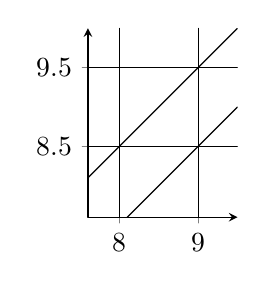
\begin{tikzpicture}[line cap=round,line join=round,,x=1cm,y=1cm]
\begin{axis}[
x=1cm,y=1cm,
axis lines=middle,
ymajorgrids=true,
xmajorgrids=true,
xmin=7.6,
xmax=9.5,
ymin=7.6,
ymax=10,
xtick={8,9},
ytick={8.5,9.5},]
\clip(7.6,6.862040816326529) rectangle (9.5,10);
\draw [domain=7.6:9.5] plot(\x,{(--9.5-0*\x)/1});
\draw [domain=7.6:9.5] plot(\x,{(--8.5-0*\x)/1});
\draw [] (8,6.862040816326529) -- (8,10);
\draw [] (9,6.862040816326529) -- (9,10);
\draw [domain=7.6:9.5] plot(\x,{(--0.5--1*\x)/1});
\draw [domain=7.6:9.5] plot(\x,{(-0.5--1*\x)/1});
\end{axis}
\end{tikzpicture}
\end{center}
\end{examplle}
\subsection{随机变量与其概率分布}
\label{sec:org3b46f96}
\begin{examplle}[]
设\(F(x)\)为随机变量\(X\)的分布函数,则成立\(P\{x_1<X<x_2\}=F(x_2)-F(x_1)\)的
充要条件是
\begin{enumerate}
\item \(x_1\)处连续
\item \(x_2\)处连续
\item \(x_1,x_2\)至少一处连续
\item \(x_1,x_2\)都不连续
\end{enumerate}


\(P\{x_1<X<x_2\}=P\{x_1<X\le x_2\}-P\{X=x_2\}=F(x_2)-F(x_1)-P\{X=x_2\}\)。
\(P\{x_1<X<x_2\}=F(x_2)-F(x_1)\)可知\(P\{X=x_2\}=0\)即\(F(x_2)-F(x_2-0)=0\),
\(F(x)\)在\(x_2\)处作连续,\(F(x)\)是右连续的,因此\(x_2\)处\(F(x)\)连续
\end{examplle}

\begin{examplle}[]
设\(X_1,X_2,X_3\)是随机变量,且\(X_1\sim N(0,1),X_2\sim N(0,2^2),X_3\sim
   N(5,3^2)\),\(p_i=P\{-2\le X_i\le 2\}\),则
\begin{enumerate}
\item \(p_1>p_2>p_3\)
\item \(p_2>p_1>p_3\)
\item \(p_3>p_1>p_2\)
\item \(p_1>p_3>p_2\)
\end{enumerate}


\(p_1=\Phi(2)-\Phi(-2)=2\Phi(2)-1\),
\(p_2=\Phi(\frac{2-0}{2})-\Phi(\frac{-2-0}{2})=\Phi(1)-\Phi(-1)=2\Phi(1)-1\),
\(p_3=\Phi(\frac{2-5}{3})-\Phi(\frac{-2-5}{3})=\Phi(-1)-\Phi(-\frac{7}{3})\),
因此 \(p_1>p_2>p_3\)
\end{examplle}

\begin{examplle}[]
设随机变量\(X\)的概率密度\(f(x)=Ae^{-x^2+x}\),试求常数\(A\)

\begin{align*}
1&=\int_{-\infty}^{+\infty}Ae^{-x^2+x}dx=Ae^{\frac{1}{4}}\int_{-\infty}^{+\infty}
e^{-(x-\frac{1}{2})^2}dx\\
&=Ae^{\frac{1}{4}}\int_{-\infty}^{+\infty}e^{-t^2}dt=Ae^{1/4}\sqrt{\pi}
\end{align*}
\end{examplle}

\begin{examplle}[]
假设随机变量\(X\)服从指数分布,则随机变量\(Y=\min\{X,2\}\)的分布函数
\begin{enumerate}
\item 是连续函数
\item 至少有两个间断点
\item 是阶梯函数
\item 恰好有一个间断点
\end{enumerate}


*方法 1*。设\(Y\)的分布函数为\(F_Y(y)\)。

当\(y<0\)时,\(F_Y(y)=0\)

当\(0\le y<2\)时
\begin{align*}
F_Y(y)&=P\{Y\le y\}=P\{\min\{X,2\}\le y\}\\
&=P\{X\le y\}=\int_{-\infty}^y\lambda e^{-\lambda x}dx=1-e^{-\lambda y}
\end{align*}

但\(y\ge2\)时,\(F_Y(y)=1\),因此
\begin{equation*}
F_Y(y)=
\begin{cases}
0&y<0\\
1-e^{-\lambda y}&0\le y<2\\
1&y\ge2
\end{cases}
\end{equation*}
因此间断点为\(y=2\)

\textbf{方法 2}.指数分布\(X\)的分布函数必为连续函数,
\begin{equation*}
F_Y(y)=P\{Y\le y\}=P\{\min\{X,2\}\le y\}=
\begin{cases}
F_X(y)&y<2\\
1&y\ge2
\end{cases}
\end{equation*}
故有一个间断点
\end{examplle}
\subsection{多维随机变量及其分布}
\label{sec:orgf57af4a}
\begin{examplle}[]
设\((X,Y)\)是二维随机变量,\(X\)的边缘概率密度为
\begin{equation*}
f_X(x)=
\begin{cases}
3x^2&0<x<1\\
0
\end{cases}
\end{equation*}
在给定\(X=x(0<x<1)\)的条件下\(Y\)的条件概率密度为
\begin{equation*}
f_{Y\mid X}(y\mid x)=
\begin{cases}
 \frac{3y^2}{x^3}&0<y<x\\
 0
\end{cases}
\end{equation*}
\begin{enumerate}
\item 求\((X,Y)\)的概率密度为\(f(x,y)\)
\item 求\(Y\)的边缘概率密度 \(f_Y(y)\)
\item 求\(P\{X>2Y\}\)
\end{enumerate}


注意条件概率是在\(X=x\)的条件下给定的,因此在\(0<x<1\)时
\begin{equation*}
f(x,y)=
\begin{cases}
\frac{3y^2}{x^3}&0<y<x\\
0
\end{cases}
\end{equation*}
又\(\int_0^1\int_{-\infty}^{+\infty}f(x,y)dy=1\)
\end{examplle}

\begin{examplle}[]
设随机变量\(X,Y\)相互独立,\(X\sim B(1,0.5),Y\sim U[0,1]\),记\(Z=X+Y\),试求
\(Z\)的概率密度\(f_Z(z)\)

\begin{align*}
F_Z(z)&=
P\{Z\le z\}=P\{X+Y\le z\}\\
&=P\{X=0,X+Y\le z\}+P\{X=1,X+Y\le z\}\\
&=P\{X=0,Y\le z\}+P\{X=1,Y\le z-1\}\\
&=\frac{1}{2}F_Y(z)+\frac{1}{2}F_Y(z-1)\\
&=
\begin{cases}
0&z<0\\
\frac{z}{2}&0\le z\le 2\\
1&2<z
\end{cases}
\end{align*}
\end{examplle}

\begin{examplle}[]
设随机变量\(X\)的概率密度为
\begin{equation*}
f(x)=
\begin{cases}
\frac{1}{9}x^2&0<x<3\\
0&\text{otherwise}
\end{cases}
\end{equation*}
令随机变量
\begin{equation*}
Y=
\begin{cases}
2&X\le1\\
X&1<X<2\\
1&2\le X
\end{cases}
\end{equation*}
\begin{enumerate}
\item 求\(Y\)的分布函数
\item 求概率\(P\{X\le Y\}\)
\end{enumerate}



\(1\le Y\le2\),因此

当\(y<1\)时,\(F_Y(y)=0\)

当\(1\le y<2\)时,
\begin{align*}
F_Y(y)&=P\{Y\le y\}=P\{Y<1\}+P\{Y=1\}+P\{1<Y\le y\}\\
&=0+P\{X\ge2\}+P\{1<X\le y\}\\
&=\int_2^3\frac{1}{9}x^2dx+\int_1^y\frac{1}{9}x^2dx=\frac{y^3+18}{27}
\end{align*}

当\(2\le y\)时,\(F_Y(y)=P\{Y\le y\}=P\{Y\le 2\}=1\)

\begin{align*}
P\{X\le Y\}&=P\{X=Y\}+P\{X<Y\}\\
&=P\{1<X<2\}+P\{X\le1\}\\
&=P\{X<2\}=\int_0^2\frac{1}{9}x^2dx=\frac{8}{27}
\end{align*}
\end{examplle}

\begin{examplle}[]
设\((X,Y)\sim N(\mu,\mu;\sigma^2,\sigma^2;0)\),则\(P\{X<Y\}=\)

\(P\{X<Y\}=\displaystyle\iint_{x<y}\frac{1}{2\pi\sigma^2}e^
   {-\frac{1}{2e^2}[(x-\mu)^2+(y-\mu)^2]}dxdy\)

用极坐标
\begin{equation*}
\begin{cases}
x-\mu=\rho\cos\theta\\
y-\mu=\rho\sin\theta
\end{cases}
\end{equation*}
则
\begin{equation*}
P\{X<Y\}=\frac{1}{2\pi\sigma^2}\int_{\frac{\pi}{4}}^{\frac{5}{4}\pi}d\theta
\int_0^{+\infty}e^{-\frac{-\rho^2}{2\sigma^2}}\rho d\rho=\frac{1}{2}
\end{equation*}

或由对称性得
\end{examplle}

\begin{examplle}[]
设随机变量\(X,Y\)相互独立,服从同一参数为 \(\lambda\) 的泊松分布,试求:随机变量
\(Z=X+Y\)的分布律

\begin{align*}
P\{Z=k\}&=P\{X+Y=k\}=\sum_{i=0}^kP\{X=i,Y=k-i\}=\sum_{i=0}^k
\frac{\lambda^i e^{-\lambda}}{i!}\frac{\lambda^{k-i}e^{-\lambda}}{(k-i)!}\\
&=e^{-2\lambda}\sum_{i=0}^k\frac{\lambda^k}{i!(k-i)!}=e^{-2\lambda}\sum_{i=0}^k
\frac{k!}{i!(k-i)!}\frac{\lambda^k}{k!}\\
&=e^{-2\lambda}\frac{\lambda^k}{k!}\sum_{i=0}^kC_k^i=e^{-2\lambda}\frac{\lambda^k}{k!}(1+1)^k\\
&=\frac{(2\lambda)^k}{k!}e^{-2\lambda},k=0,1,\dots
\end{align*}
\end{examplle}

\begin{examplle}[]
设随机变量\(X_i\)的概率分布为
\begin{center}
\begin{tabular}{l|rrr}
\(X_i\) & 0 & 1 & 2\\
\hline
\(P\) & \(\frac{1}{2}\) & \(\frac{1}{4}\) & \(\frac{1}{4}\)\\
\end{tabular}
\end{center}
\(i=1,2\),且满足\(P\{X_1X_2=0\}=1\),则\(P\{X_1=X_2\}=\)

\begin{center}
\begin{tabular}{r|lrr|l}
\(X_1\textbackslash X_2\) & 0 & 1 & 2 & \\
\hline
0 & 0 & \(\frac{1}{4}\) & \(\frac{1}{4}\) & \(\frac{1}{2}\)\\
1 & \(\frac{1}{4}\) & 0 & 0 & \(\frac{1}{4}\)\\
2 & \(\frac{1}{4}\) & 0 & 0 & \(\frac{1}{4}\)\\
\hline
 & \(\frac{1}{2}\) & \(\frac{1}{4}\) & \(\frac{1}{4}\) & \\
\end{tabular}
\end{center}
\end{examplle}

\begin{examplle}[]
设\(F_1(x)\)和\(F_2(x)\)为二维随机变量\((X_1,X_2)\)的边缘分布函数,且
\(X_1,X_2\)相互独立,则
\begin{enumerate}
\item \(2F_1(x)-F_2(x)\)必为某一随机变量的分布函数
\item \(F_1(x)+F_2(x)\)必为某一随机变量的分布函数
\item \(F_1(x)-\frac{1}{2}F_2(x)\)必为某一随机变量的分布函数
\item \(F_1(x)F_2(x)\)必为某一随机变量的分布函数
\end{enumerate}


\(F(x)\)分布函数的充要条件是
\begin{enumerate}
\item 单调不减
\item \(\displaystyle\lim_{x\to-\infty}F(x)=0,\lim_{x\to+\infty}F(x)=1\)
\item 右连续
\end{enumerate}
\end{examplle}
\subsection{随机变量的数字特征}
\label{sec:org6ff7e3b}
\begin{examplle}[]
设随机变量\(X\)的分布函数为\(F(x)=0.3\Phi(x)+0.7\Phi(\frac{x-1}{2})\),其中
\(\Phi(x)\)为标准正态分布函数,求\(E(X)\)

*方法 1*。\(f(x)=F'(x)=0.3\varphi(x)+\frac{0.7}{2}\varphi(\frac{x-1}{2})\),其中
 \(\varphi(x)\)为标准正态密度函数
\begin{align*}
E(X)&=\int_{-\infty}^{+\infty}xf(x)dx=0.3\int_{-\infty}^{+\infty}x\varphi(x)dx+
\frac{0.7}{2}\int_{-\infty}^{+\infty}x\varphi(\frac{x-1}{2})dx\\
&=0.3+0.7\int_{-\infty}^{+\infty}(2t+1)\varphi(t)dt=0.7
\end{align*}

*方法 2*。当\(X\sim N(\mu,\sigma^2)\)时,其分布函数为\(\Phi(\frac{x-\mu}{\sigma})\),即有分布
 函数为\(\Phi(\frac{x-\mu}{\sigma})\)的随机变量,其数学期望是 \(\mu\) ,故
 \(F(x)=0.3\Phi(x)+0.7\Phi(\frac{x-1}{2})\)的数学期望为\(0.7\)
\end{examplle}

\begin{examplle}[]
已知\(N\)件产品中含有\(M\)件次品,从中任意一次取出\(n\)件(\(n\le N\)),设这
\(n\)件产品中的次品件数为\(X\),试求\(X\)的数学期望\(E(X)\)

将一次取出\(n\)件理解成一次一件地不放回地取\(n\)次
令
\begin{equation*}
X_i=
\begin{cases}
1&\text{第$i$次取得次品}\\
0&\text{第$i$次取得正品}
\end{cases}
i=1,2,\dots,n
\end{equation*}
显然\(X=\displaystyle\sum_{i=1}^nX_i\),第\(i\)次取得次品的概率,无论每次取后
放回或不放回,均为\(\frac{M}{N}\),因此
\begin{equation*}
E(X)=\sum_{i=1}^nE(X_i)=n\frac{M}{N}
\end{equation*}
\end{examplle}

\begin{examplle}[]
设随机变量\(X,Y\)独立同分布,已知\(X\sim N(\mu,\sigma^2)\),求\(Z=\min(X,Y)\)的数学
期望\(E(Z)\)

设\(\xi=\frac{X-\mu}{\sigma},\eta=\frac{Y-\mu}{\sigma}\)
\begin{align*}
Z&=\min(X,Y)=\min(\sigma\xi+\mu,\sigma\eta+\mu)=\sigma\min(\xi,\eta)+\mu\\
E[\min(\xi,\eta)]&=
\int_{-\infty}^{+\infty}\int_{-\infty}^{+\infty}\min(x,y)\frac{1}{2\pi}e^{-\frac{x^2+y^2}{2}}dxdy\\
&=\frac{1}{2\pi}\int_{-\infty}^{+\infty}e^{-\frac{x^2}{2}}dx\int_{-\infty}^xye^{-\frac{y^2}{2}}dy+
\frac{1}{2\pi}\int_{-\infty}^{+\infty}e^{-\frac{y^2}{2}}dy
\int_{-\infty}^yxe^{-\frac{x^2}{2}}dx\\
&=2\frac{1}{2\pi}\int_{-\infty}^{+\infty}(-1)e^{-x^2}=-\frac{1}{\sqrt{\pi}}
\end{align*}
因此
\begin{equation*}
E(Z)=\sigma E[\min(\xi,\eta)]+\mu=\mu-\frac{\sigma}{\sqrt{\pi}}
\end{equation*}
\end{examplle}

\begin{examplle}[]
设随机变量\(X\)的概率密度函数为
\begin{equation*}
f(x)=Ae^{-\frac{x^2}{2}+Bx},-\infty<x<+\infty
\end{equation*}
其中\(A,B\)为常数,已知\(E(X)=D(X)\),试求\(A,B,E(X)\)

\(f(x)=Ae^{\frac{B^2}{2}}e^{-\frac{(x-B)^2}{2}}\),该密度是正态分布\(N(B,1)\)的
密度函数

又因为\(E(X)=D(X)\),因此\(B=1\)
\end{examplle}

\begin{examplle}[]
将\(n\)只球相互独立地放入到\(N\)只盒子中,设每只球放入各个盒子是等可能的,求
有球的盒子数\(X\)的数学期望\(E(X)\)

设
\begin{equation*}
X_i=
\begin{cases}
1&\text{第$i$只盒子有球}\\
0&\text{第$i$只盒子无球}
\end{cases}
\end{equation*}
显然\(X=\sum_{i=1}^NX_i\)

对第\(i\)只盒子而言,一只球放入的概率为\(\frac{1}{N}\),没放入的概率为
\((1-\frac{1}{N})\),因此
\begin{gather*}
P\{X_i=0\}=\left(1-\frac{1}{N}\right)^n\\
P\{X_i=1\}=1-\left(1-\frac{1}{N}\right)^n\\
E(X_i)=1-\left(1-\frac{1}{N}\right)^n
\end{gather*}
因此
\begin{equation*}
E(X)=N\left[1-\left(1-\frac{1}{N}\right)^n\right]
\end{equation*}
\end{examplle}

\begin{examplle}[]
设随机变量\(X,Y\)的联合分布在以点\((0,1),(1,0),(1,1)\)为 顶点的三角形上服从均
匀分布,试求随机变量\(U=X+Y\)的方差

以\(f_U(u)\)表示\(U=X+Y\)的概率密度,当\(u<1\)或\(u>2\)时,显然
\(f_U(u)=0\),设\(1\le u\le2\),当\(0\le x\le 1\)时且\(0\le u-x\le1\),
\(f(x,u-x)=2\),因此
\begin{equation*}
f_U(u)=\int_{-\infty}^{+\infty}f(x,u-x)dx=\int_{u-1}^12dx=2(2-u)
\end{equation*}
因此
\begin{align*}
&E(X+Y)=E(U)=\int_{-\infty}^{+\infty}uf_U(u)=2\int_1^2u(2-u)du=\frac{4}{3}\\
&E((X+Y)^2)=\int_{-\infty}^{+\infty}u^2f(u)du=2\int_1^2u^2(2-u)du=\frac{11}{6}\\
&D(U)=\frac{11}{6}-\frac{16}{9}=\frac{1}{18}
\end{align*}
\end{examplle}

\begin{examplle}[]
已知随机变量\((X,Y)\)服从二维正态分布\(N\left(1,0;9,16;-\frac{1}{2}\right)\),
设\(Z=\frac{X}{3}+\frac{Y}{2}\)
\begin{enumerate}
\item 求\(Z\)的数学期望\(E(Z)\)和方差\(D(Z)\)
\item 求\(X,Z\)的相关系数\(\rho_{XZ}\)
\item 问\(X,Z\)是否相互独立
\end{enumerate}


\((X,Y)\sim N\left(1,0;9,16;-\frac{1}{2}\right)\),所以\(X\sim N(1,9),Y\sim
   N(0,16),\rho_{XY}=-\frac{1}{2}\).
\begin{align*}
E(Z)&=E(\frac{X}+\frac{Y}{3})=\frac{1}{3}\\
D(Z)&=D(\frac{X}{3}+\frac{Y}{2})=\frac{D(X)}{9}+\frac{D(Y)}{4}+2Cov(\frac{X}{3},\frac{Y}{2})\\
&=1+4+\frac{\rho_{XY}}{\sqrt{D(X)}\sqrt{D(Y)}}=1+4-2=3
\end{align*}

\begin{align*}
Cov(X,Z)&=\frac{1}{3}Cov(X,X)+\frac{1}{2}Cov(X,Y)\\
&=\frac{1}{3}D(X)+\frac{1}{2}\frac{\rho_{XY}}{\sqrt{D(X)}\sqrt{D(Y)}}=0
\end{align*}

因为\((X,Y)\)是正态分布,故\((X,\frac{X}{3}+\frac{Y}{2})\)也是正态分布且
\(\rho_{XZ}=0\),因此独立
\end{examplle}

\begin{examplle}[]
设随机变量\(X,Y\)的数学期望都是 2,方差分别为 1,4,相关系数 0.5,则根据切比雪夫
不等式\(P\{\abs{X-Y}\ge 6\}\le\und{\hspace{1cm}}\)

令\(Z=X-Y\),则\(E(Z)=0,D(Z)=D(X-Y)=D(X)+D(Y)-2Cov(X,Y)=3\),因此
\begin{equation*}
P\{\abs{X-Y}\ge6\}=P\{\abs{E-E(Z)}\ge6\}\le\frac{D(Z)}{6^2}=\frac{1}{12}
\end{equation*}
\end{examplle}

\begin{examplle}[]
某种电子元件的寿命\(E\sim E(\lambda)\),现有\(n\)个该钟元件相互独立工作,已知其中至
少有一个工作元件寿命超过平均寿命的概率为\(3e^{-1}-3e^{-2}+e^{-3}\),求\(n\)

\(EX=\frac{1}{\lambda}\),每个元件工作寿命不超过平均寿命的概率为
\(P\{X\le EX\}=P\{X\le\frac{1}{\lambda}\}=1-e^{-1}\)
\end{examplle}

\begin{examplle}[]
游客乘电梯观光,电梯于每个整点的第 5,25,55 分钟从底层起行,假设一游客在早上 8
点的第\(X\)分钟到达底层候梯处,且\(X\)服从\([0,60]\)的均匀分布,求该乘客等候
时间的数学期望

设游客等候时间为\(Y\),则
\begin{equation*}
Y=
\begin{cases}
5-X&0\le X\le 5\\
25-X&5<X\le25\\
55-X&25<X\le 55\\
65-X&55<X\le60
\end{cases}
\end{equation*}
因此
\begin{align*}
E(Y)&=E[g(X)]=\int_0^5(5-x)\frac{1}{60}dx+\int_5^{25}(25-x)\frac{1}{60}dx\\
&+\int_{25}^{55}(55-x)\frac{1}{60}dx+\int_{55}^{60}(65-x)\frac{1}{60}dx\\
&=\frac{35}{3}
\end{align*}
\end{examplle}

\begin{examplle}[]
某线路有两个中间站,设两个中间站无故障的时间分别为\(X_1,X_2\),均服从指数分布,
已知它们平均无故障工作时间为 1 和 0.5(千小时),求线路无故障工作时间的期望

\(X_1\sim E(1),X_2\sim E(2)\)
\begin{align*}
E(Y)&=\int_{-\infty}^{\infty}\int_{-\infty}^{\infty}\min\{x_1,x_2\}f_1(x_1)f_2(x_2)dx_1dx_2\\
&=\int_0^{+\infty}dx_1\int_{x_1}^{+\infty}x_1e^{-x_1}2e^{-2x_2}dx_2+
+\int_0^{+\infty}dx_2\int_{x_2}^{+\infty}x_2e^{-x_1}2e^{-2x_2}dx_1\\
&=\frac{1}{9}+\frac{2}{9}=\frac{1}{3}
\end{align*}
\end{examplle}
\subsection{大数定律和中心极限定理}
\label{sec:orge88bf28}
\begin{examplle}[]
\begin{enumerate}
\item 某系统由 100 个部件组成,运行期间每个部件是否损坏是相对独立的,虽坏的概率均
为 0.1,如果有 85 个以上的部件完好时系统才能正常工作,求系统正常工作的概率
\item 如果上述系统由\(n\)个部件组成,需\(80\%\)以上的部件完好时系统才能正常工作,
问\(n\)至少多大时才能使系统正常工作地概率不小于 0.95
\end{enumerate}


设
\begin{equation*}
X_k=
\begin{cases}
1&\text{第$k$个元件完好}\\
0&\text{第$k$个元件损坏}
\end{cases},k=1,2,\dots,100
\end{equation*}
\(X\)为系统正常运行时完好的元件数,\(X\sim B(100,0.9)\),\(E(X)=90,D(X)=9\)

根据中心极限定理,系统正常工作的概率为
\begin{align*}
P\{X>85\}&=1-P\{X\le85\}=1-P\left\{\frac{X-90}{\sqrt{9}}\le\frac{85-90}{\sqrt{9}}\right\}\\
&\approx 1-\Phi(-\frac{5}{3})=0.9525
\end{align*}
\begin{align*}
P\{X>0.8n\}&=1-P\{X\le 0.8n\}\\
&=1-P\left\{\frac{X-0.9n}{0.3\sqrt{n}}\le\frac{0.8n-0.9n}{0.3\sqrt{n}}\right\}\\
&\approx1-\Phi(-\frac{\sqrt{n}}{3})=\Phi(\frac{\sqrt{n}}{3})
\end{align*}
\end{examplle}
\subsection{数理统计的基本概念}
\label{sec:org2b7b962}
\begin{remark}
如果总体\(X\)的分布为\(F(x)\),则样本\(X_1,\dots,X_n\)的分布为
\begin{equation*}
F_n(x_1,\dots,x_n)=\prod_{i=1}^nF(x_i)
\end{equation*}
如果总体\(X\)有概率密度\(f(x)\),则样本\(X_1,\dots,X_n\)的概率密度为
\begin{equation*}
f_n(x_1,\dots,x_n)=\prod_{i=1}^nf(x_i)
\end{equation*}
如果总体\(X\)有概率分布\(P\{X=a_j\}=p_j\),则样本\(X_1,\dots,X_n\)的概率分布
为
\begin{equation*}
P\{X_1=x_1,\dots,X_n=x_n\}=\prod_{i=1}^nP\{X_i=x_i\}
\end{equation*}
\end{remark}

\begin{examplle}[]
设总体\(X\sim P(\lambda)\),则来自总体\(X\)的样本\(X_1,\dots,X_n\)的样本均值
\(\bbar{X}\)的分布律为

当\(X_1,\dots,X_n\)独立同为\(P(\lambda)\)分布时
\(\displaystyle\sum_{i=1}^nX_i=n\bbar{X}\sim P(n\lambda)\),因此对于任意
\(n>2\),得\(n\bbar{X}\)的分布律
\begin{equation*}
P\{n\bbar{X}=k\}=\frac{(n\lambda)^k}{k!}e^{-n\lambda},\quad
k=01,2,\dots
\end{equation*}
而\(P\{n\bbar{X}=k\}=P\{\bbar{X}=\frac{k}{n}\}\)
\end{examplle}

\begin{examplle}[]
设\(X_1,X_2,X_3,X_4\)是来自正态总体\(N(0,2^2)\)的简单随机样本,
\(X=a(X_1-2X_2)^2+b(3X_3-4X_4)^2\),则当
\(a=\und{\hspace{1cm}},b=\und{\hspace{1cm}}\)时,统计量\(X\)服从\(\chi^2\)分布,
其自由度为\(\und{\hspace{1cm}}\)

\begin{equation*}
(X_1-2X_2)\sim N(0,20),\quad(3X_3-4X_4)\sim N(0,100)
\end{equation*}
且\((X_1-2X_2),(3X_3-4X_4)\)相互独立,标准化得
\begin{equation*}
\frac{1}{\sqrt{20}}(X_1-2X_2)\sim N(0,1),\quad
\frac{1}{19}(3X_3-4X_4)\sim N(0,1)
\end{equation*}
因此当\(a=\frac{1}{20},b=\frac{1}{100}\)时,服从\(\chi^2(2)\)分布
\end{examplle}

\begin{examplle}[]
设随机变量\(T\sim t(n)\),则\(T^2\)服从的分布及参数为

\(X\sim N(0,1),X^2\sim\chi^2(1),T^2\sim F(1,n)\)
\end{examplle}

\begin{examplle}[]
已知\(X_1,X_2,X_3\)相互独立且服从\(N(0,\sigma^2)\),证明
\(\displaystyle\frac{2}{3}\frac{X_1+X_2+X_3}{\abs{X_2-X_3}}\)服从\(t(1)\)分布

记\(Y_1=X_2+X_3,Y_2=X_2-X_3\),则
\begin{align*}
Cov(Y_1,Y_2)&=
E(Y_1Y_2)-E(Y_1)E(Y_2)=E(X_2+X_3)(X_2-X_3)\\
&=EX_2^2-EX_3^2=\sigma^2-\sigma^2=0
\end{align*}
所以\(Y_1,Y_2\)独立,均服从\(N(0,2\sigma^2)\),且与\(X_1\)独立
\begin{equation*}
X_1+X_2+X_3=X_1+Y_1\sim N(0,3\sigma^2)
\end{equation*}
所以\(\displaystyle\frac{1}{\sigma\sqrt{3}}(X_1+X_2+X_3)\sim N(0,1)\),
\(\displaystyle\left(\frac{X_2-X_3}{\sqrt{2}\sigma}\right)^2\sim\chi^2(1)\),且
\(X_1+X_2+X_3\)与\(X_3-X_3\)相互独立,
\end{examplle}

\begin{examplle}[]
设总体\(X\)服从正态分布\(N(\mu,\sigma^2)\),从该总体中抽取简单随机样本
\(X_1,\dots,X_{2n}\),其样本均值为
\(\displaystyle\bbar{X}=\frac{1}{2n}\sum_{i=1}^{2n}X_i\),求统计量
\(Y=\displaystyle\sum_{i=1}^n(X_i+X_{n+i}-2\bbar{X})\)的数学期望

*方法 1*。考虑\((X_1+X_{n+1}),\dots,(X_n,X_{2n})\),将其视为取自总体
\(N(2\mu,2\sigma^2)\)的简单随机样本,样本方差为\(\frac{1}{n-1}Y\),由于
\(E(\frac{1}{n-1}Y)=2\sigma^2\),因此\(E(Y)=2(n-1)\sigma^2\)

*方法 2*。记
\(\bbar{X}'=\displaystyle\frac{1}{n}X_i,\bbar{X}''=\frac{1}{n}\sum_{i=1}^nX_{n+i}\)
有\(2\bbar{X} =\bbar{X}'+\bbar{X}''\),因此
\begin{align*}
E(Y)&=E[\sum_{i=1}^n(X_i+X_{n+i}-2\bbar{X})^2]=
E\left\{\sum_{i=1}^n\left[(X_i-\bbar{X}')+(X_{n+i}-\bbar{X}'')\right]\right\}\\
&=E\left\{\sum_{i=1}^n\left[(X_i-\bbar{X}')^2+2(X_i-\bbar{X}')(X_{n+i}-\bbar{X}'')+
(X_{n+i}-\bbar{X}'')^2\right]\right\}\\
&=E[\sum_{i=1}^n(X_i-\bbar{X}')^2]+0+E[\sum_{i=1}^n(X_{n+i}-\bbar{X}'')^2]\\
&=(n-1)\sigma^2+(n-1)\sigma^2=2(n-1)\sigma^2
\end{align*}
\end{examplle}

\begin{examplle}[]
设随机变量\(X_1,\dots,X_n\)独立同分布且具有相同的分布密度,证明
\begin{equation*}
P\{X_n>\max(X_1,\dots,X_{n-1})\}=\frac{1}{n}
\end{equation*}

设\(f(x),F(x)\)分别表示\(X_i\)共同的概率密度和分布函数,则
\begin{align*}
P\{X_n&>\max(X_1,\dots,X_{n-1})\}=P\{X_1<X_n,\dots,X_{n-1}<X_n\}\\
&=\int_{-\infty}^{+\infty}\left[\idotsint_{x_i<x_n}\prod_{i=1}^{n-1}f(x_i)dx_i\right]f(x_n)dx_n\\
&=\int_{-\infty}^{+\infty}\left[\prod_{i=1}^{n-1}\int_{-\infty}^{x_n}f(x_i)dx_i
\right]f(x_n)dx_n\\
&=\int_{-\infty}^{+\infty}F^{n-1}(x_n)f(x_n)dx_n=\frac{1}{n}F^n(x_n)
\Big\rvert_{-\infty}^{+\infty}=\frac{1}{n}
\end{align*}
\end{examplle}
\subsection{参数估计}
\label{sec:org9474af4}
\begin{examplle}[]
设\(X_1,\dots,X_n\)是来自总体\(X\)的样本,已知\(X\sim P(\lambda)\),证明
\(T=\left(1-\frac{1}{n}\right)^{n\bbar{X}}\)的数学期望是\(P\{X=0\}\)

\(P\{X=0\}=e^{-\lambda},n\bbar{X}\sim P(n\lambda)\),故
\begin{align*}
E(T)&=E\left[\left(1-\frac{1}{n}\right)^{n\bbar{X}}\right]=
\sum_{i=0}^{+\infty}\left(1-\frac{1}{n}\right)^i\frac{(n\lambda)^ie^{-n\lambda}}{i!}\\
&=e^{-n\lambda}\sum_{i=0}^{+\infty}\frac{[(n-1)\lambda]^i}{i!}\\
&=e^{-n\lambda}e^{(n-1)\lambda}=e^{-\lambda}
\end{align*}
\end{examplle}

\begin{examplle}[]
设\(X_1,\dots,X_n(n>2)\)为来自总体\(N(0,\sigma^2)\)的简单随机样本,\(\bbar{X}\)为
样本均值,记\(Y_i=X_i-\bbar{X},i=1,2,\dots,n\)求
\begin{enumerate}
\item \(Y_i\)的方差\(DY_i\)
\item \(Cov(Y_1,Y_n)\)
\item 当\(C(Y_1+Y_n)^2\)的数学期望为 \(\sigma^2\)时的常数\(C\)
\item \(P\{Y_1+Y_n\le0\}\)
\end{enumerate}


\begin{align*}
Cov(Y_1,Y_n)&=EY_1Y_2-EY_1\cdot EY_n=EY_1Y_2=E(X_1-\bbar{X})(X_n-\bbar{X})\\
&=E(X_1X_n)-E(X_1\bbar{X})-E(X_n\bbar{X})+E(\bbar{X}^2)\\
&=EX_1EX_n-2E(X_1\bbar{X})+D\bbar{X}+(E\bbar{X})^2\\
&=0-2\frac{1}{n}E(X_1^2+\sum_{j=2}^nX_1X_j)+D(\bbar{X})+0\\
&=-\frac{2}{n}(\sigma^2+0)+\frac{1}{n}\sigma^2=-\frac{\sigma^2}{n}
\end{align*}

\begin{align*}
Y_1+Y_2&=X_1+X_n-2\bbar{X}=\\
&=\frac{n-2}{n}X_1-\frac{2}{n}\sum_{n=2}^{n-1}X_i+\frac{n-2}{n}X_n
\end{align*}
服从正态分布,因此\(Y_1+Y_2\sim N(0,\cdot)\),因此\(P\{Y_1+Y_2\le0\}=0.5\)
\end{examplle}

\begin{examplle}[]
设\(X_1,\dots,X_n\)是总体\(N(\mu,\sigma^2)\)的简单随机样本,记
\(\bbar{X}=\displaystyle\sum_{i=1}^nX_i\),
\(S^2=\frac{1}{n-1}\displaystyle\sum_{i=1}^n(X_i-\bbar{X})^2\)和
\(T=\bbar{X}^2-\frac{1}{n}S^2\),求
\begin{enumerate}
\item 统计量\(T\)的数学期望
\item 当\(\mu=0,\sigma=1\)时的统计量\(T\)的方差
\end{enumerate}


\begin{enumerate}
\item \(\mu^2\)
\item \(\bbar{X}\sim N(0,\frac{1}{n})\),因此\(n\bbar{X}\sim\chi^2(1)\)和
\((n-1)S^2\sim t(n-1)\),注意到\(\bbar{X}\)与\(S\)相互独立,且
\(D(\chi^2(n))=2n\)
\begin{align*}
D(T)&=D(\bbar{X}^2-\frac{1}{n}S^2)=D(\bbar{X}^2)+\frac{1}{n^2}D(S^2)\\
&=\frac{1}{n^2}D(n\bbar{X}^2)+\frac{1}{n^2}\frac{1}{(n-1)^2}D[(n-1)S^2]\\
&=\frac{1}{n^2}\cdot 2+\frac{1}{n^2(n-1)^2}\cdot 2(n-1)\\
&=\frac{2}{n(n-1)}
\end{align*}
\end{enumerate}
\end{examplle}

\begin{examplle}[]
设总体\(X\)的概率分布为
\begin{center}
\begin{tabular}{l|rrr}
\(X\) & 1 & 2 & 3\\
\hline
\(P\) & \(1-\theta\) & \(\theta-\theta^2\) & \(\theta^2\)\\
\end{tabular}
\end{center}

其中参数\(\theta\in(0,1)\)未知,以\(N_i\)表示来自总体\(X\)的简单随机样本(样
本容量为\(n\))中等于\(i\)的个数,试求\(a_1,a_2,a_3\)使统计量
\(T=\displaystyle\sum_{i=1}^3a_iN_i\)的数学期望为 \(\theta\) ,并求\(T\)的方差

记\(p_1=1-\theta,p_2=\theta-\theta^2,p_3=\theta^2\),则\(N_i\sim B(n,p_i)\),
因此\(E(T)=\displaystyle\sum_{i=1}^3a_inp_i=\theta\),因此
\(a_1=0,a_2=\frac{1}{n}=a_3\),\(T=\frac{1}{n}(N_2+N_3)\)

显然\(N_2+N_3\)不独立,但\(N_1+N_2+N_3=n\),因此\(T=\frac{1}{n}(n-N_1)\)
\end{examplle}

\begin{examplle}[]
设总体\(X\)的分布函数
\begin{equation*}
F(x;\theta)=
\begin{cases}
1-e^{-\frac{x^2}{\theta}}&x\ge0\\
0&x<0
\end{cases}
\end{equation*}
其中 \(\theta\) 是未知参数且大于零,\(X_1,\dots,X_n\)为来自总体\(X\)的简单随机样本
\begin{enumerate}
\item 求\(EX\)与\(EX^2\)
\item 求\(\theta\)的最大似然估计量\(\hat{\theta}_n\)
\item 是否存在实数\(a\),使得对任何\(\epsilon>0\)都有
\(\displaystyle\lim_{n\to\infty}P\{\abs{\hat{\theta}_n-a}\ge\epsilon\}=0\)
\end{enumerate}


\begin{equation*}
f(x;\theta)=
\begin{cases}
\frac{2x}{\theta}e^{-\frac{x^2}{\theta}}
\end{cases}
\end{equation*}
\begin{enumerate}
\setcounter{enumi}{1}
\item 设\(x_1,\dots,x_n\)为样本观察值,似然函数为
\begin{equation*}
L(\theta)=\prod_{i=1}^nf(x_i;\theta)=
\begin{cases}
\frac{2^nx_1\dots x_n}{\theta^n}e^{-\frac{1}{\theta}\sum_{i=1}^nx_i^2}
&x_1,\dots,x_n>0\\
0
\end{cases}
\end{equation*}
当\(x_1,\dots,x_n>0\)时,\(\ln L(\theta)=n\ln2+\displaystyle\sum_{i=1}^n\ln
      x_i-n\ln\theta-\frac{1}{\theta}\sum_{i=1}^nx_i^2\)
令\(\frac{d\ln L(\theta)}{d\theta}=0\),有\(\hat{\theta}_n=\frac{1}{n}\displaystyle\sum_{i=1}^nX_i^2\)
\item 根据辛钦大数定理,当\(n\to\infty\)时,\(\frac{1}{n}\sum_{i=1}^nX_i^2\)依概
率收敛于\(EX_i^2=\theta\),因此存在实数\(a=\theta\)
\end{enumerate}
\end{examplle}



\section{附录}
\label{sec:org9a54899}
\subsection{微积分}
\label{sec:orgeb4dda0}
   \begin{equation*}
\sec\alpha=\frac{1}{\cos\alpha},\quad\csc\alpha=\frac{1}{\sin\alpha}
\end{equation*}

Suppose we have two units \(\vec{u}=(\cos x,\sin x),\vec{v}=(\cos y,\sin
   y)\), then
\begin{equation*}
\vec{u}\cdot\vec{v}=\cos x\cos y+\sin x\sin y=\cos(x-y)
\end{equation*}
Hence by substitute \(-y\) for \(y\) or \(\frac{\pi}{2}-x\) for \(x\), we have
\begin{gather*}
\cos(x+y)=\cos x\cos y-\sin x\sin y\\
\sin(x+y)=\sin x\cos y+\cos x\sin y\\
\sin(x-y)=\sin x\cos y-\cos x\sin y
\end{gather*}

let \(x=y\), we have
\begin{gather*}
\sin 2x=2\sin x\cos x\\
\cos 2x=\cos^2x-\sin^2x=1-2\sin^2 x=2\cos^2-1\\
\tan 2x=\frac{2\tan x}{1-\tan^2x}
\end{gather*}
Hence we have
\begin{gather*}
\sin^2\frac{x}{2}=\frac{1-\cos x}{2}\\
\cos^2\frac{x}{2}=\frac{1+\cos x}{2}\\
\tan^2\frac{x}{2}=\frac{1-\cos x}{1+\cos x}
\end{gather*}

\begin{equation*}
\tan\frac{x}{2}=\frac{\sin\frac{x}{2}}{\cos\frac{x}{2}}=
\frac{2\sin^2\frac{x}{2}}{2\sin\frac{x}{2}\cos\frac{x}{2}}=
\frac{1-\cos x}{\sin x}=\csc x-\cot x
\end{equation*}

\textbf{点到直线的距离}

设直线的方程为\(l:Ax+By+C=0\),\(A,B\neq0\),点的坐标为\(P(x_0,y_0)\),点
\(P\)到\(l\)的距离为\(d\)。在该直线上任取一点\(R(x,y)\),直线法向量为
\(\vv{n}=(A,B)\),\(\vv{PR}=(x-x_0,y-y_0)\),所欲求的\(d\)为\(\vv{PR}\)
在\(\vv{n}\)上的投影,于是有
\begin{equation*}
d=\frac{\abs{\vv{PR}\cdot\vv{PQ}}}{\abs{\vv{PQ}}}=
\frac{\abs{A(x-x_0)+B(y-y_0)}}{\sqrt{A^2+B^2}}=\frac{\abs{Ax_0+By_0+C}}{\sqrt{A^2+B^2}}
\end{equation*}

对于
\begin{equation*}
y''+py'+qy=f(x)
\end{equation*}
\begin{enumerate}
\item 求特征方程\(\lambda^2+p\lambda+q=0\)的根
\begin{enumerate}
\item 若特征方程有相异实根\(\lambda_1,\lambda_2\),通解为\(y_0(x)=C_1e^{\lambda_1x}+C_2e^{\lambda_2x}\)
\item 若特征方程有重根 \(\lambda\) ,则通解为\(y_0(x)=(C_1+C_2x)e^{\lambda x}\)
\item 若特征方程有共轭复根\(\alpha\pm i\beta(\beta\neq0)\),则通解为
\begin{equation*}
y_0(x)=e^{\alpha x}(C_1\cos\beta x+C_2\sin\beta x)
\end{equation*}
\end{enumerate}
\item 根据非齐次项\(f(x)\)的形式再求特解\(y^*(x)\)

\begin{tabular}{|c|l|}
\hline
\(f(x)\)的类型&特解\(y^*(x)\)的形式 \\\hline
\(f(x)=P_n(x)\)&1. 0不是特征方程的根,\(y^*(x)=R_n(x)\),其中\\
其中\(P_n(x)\)为\(x\)的&\(R_n(x)\)为待定的\(x\)的\(n\)次多项式\\
\(n\)次多项式&2. 0不是特征方程的但根,\(y^*(x)=xR_n(x)\)\\
&3. 0不是特征方程重根,\(y^*(x)=x^2R_n(x)\)\\\hline
&1. (\alpha)不是特征方程的根,\(y^*(x)=e^{\alpha x}R_n(x)\),其中\\
&\(R_n(x)\)为待定的\(x\)的\(n\)次多项式\\
\(f(x)=P_n(x)e^{\alpha x}\)&2. \(\alpha\)是特征方程的单根,\(y^*(x)=xe^{\alpha x}R_n(x)\)\\
&3. \(\alpha\)是特征方程的重根,\(y^*(x)=x^2e^{\alpha x}R_n(x)\)\\\hline
\(f(x)=A_0\sin\beta x\)&1. \(i\beta\) 不是特征方程的根,\(y^*(x)=A\cos\beta x+B\sin\beta x\)\\
或\(B_0\cos\beta x\)&2. \(i\beta\)是特征方程的根,\(y^*(x)=x(A\cos\beta x+B\sin\beta x)\)\\
&其中\(A,B\)为待定系数\\\hline
\end{tabular}
\end{enumerate}



对\(y_t=f(t)\),\(n\)阶差分
\begin{equation*}
\Delta^ky_t=\Delta^{k-1}y_{t+1}-\Delta^{t-1}y_t=
\sum_{i=0}^k(-1)^i\binom{k}{i}y_{t+k-i}
\end{equation*}
形如\(y_{t+1}-py_t=f(t)\)的方程称为一阶常系数线性差分方程,其中\(p\)为非零系
数,\(f(t)\)为已知函数。\(y_{t+1}-py_t=0\)称为它对应的常系数一阶线性齐次差分
方程。

一阶常系数线性差分方程的通解为\(y_t=kp^t+y_t^*\),其中\(y^*_t\)为特解

若\(f(t)=(A_0t^n+\dots+A_n)b^t\),则待定特解\(y^*_t\)具有下列形式
\begin{equation*}
y_t^*=t^s(B_0t^n+\dots+B_n)b^t
\end{equation*}
当\(p\neq b\)时,\(s=0\),当\(p=b\)时,\(s=1\)

\(I=\int_{-\infty}^\infty e^{-x^2}dx=\sqrt{\pi}\)
\begin{align}
I^2 &= \iint e^{-(r^2)}r\,d\theta\,dr \\
&=\int_0^{2\pi}\left(\int_0^\infty re^{-r^2}dr\right)d\theta \\
&=2\pi\int_0^\infty re^{-r^2}dr
\end{align}

\subsection{线性代数}
\label{sec:org54c9cc4}
\begin{equation*}
\begin{vmatrix}
\bzero&\bA\\\bB&*
\end{vmatrix}=
\begin{vmatrix}
*&\bA\\\bB&\bzero
\end{vmatrix}=
(-1)^{mn}\abs{\bA}\cdot\abs{\bB}
\end{equation*}

\begin{equation*}
(k\bA)^{-1}=\frac{1}{k}\bA^{-1},\abs{\bA^{-1}}=\frac{1}{\abs{\bA}}
\end{equation*}
伴随矩阵的性质
\begin{align*}
&(\bA^*)^{-1}=(\bA^{-1})^*=\frac{\bA}{\abs{\bA}}(\abs{\bA}\neq0)\\
&(\bA^*)^T=(\bA^T)^*\\
&(k\bA)^*=k^{n-1}\bA^*\\
&\abs{\bA^*}=\abs{\bA}^{n-1};(\bA^*)^*=\abs{\bA}^{n-2}\bA
\end{align*}

\begin{equation*}
(k\bA)=\frac{1}{k}\bA^{-1}
\end{equation*}

if \(A\) and \(B\) are square matrices s.t. \(AB=I\), where \(I\) is the
identity matrix, show that \(BA=I\). See \href{https://math.stackexchange.com/questions/3852/if-ab-i-then-ba-i}{Proof}


给定数域\(K\)上\(m\times n\)矩阵\(A\)和\(n\times s\)矩阵\(B\),则
\begin{equation*}
r(AB)\ge r(A)+r(B)-n
\end{equation*}

相似的矩阵有相同的特征多项式

\begin{equation*}
r(\bA^*)=
\begin{cases}
n&r(\bA)=n\\
1&r(\bA)=n-1\\
0&r(\bA)<n-1
\end{cases}
\end{equation*}
\href{https://math.stackexchange.com/questions/410402/for-given-n-times-n-matrix-a-singular-matrix-prove-that-operatornamerank/410415\#410415}{Proof}

当\(\balpha_1,\dots,\balpha_n\)线性无关时,向量组
\(\balpha_1+\balpha+2,\dots,\balpha_{n-1}+\balpha_n, \balpha_n+\balpha_1\)当
\(n=2k\)时线性相关,当\(n=2k+1\)时线性无关

设\(\bA=[a_{ij}]_{n\times n},\lambda_i(i=1,2,\dots,n)\)是\(\bA\)的特征值,则
\begin{enumerate}
\item \(\sum_{i=1}^n\lambda_i=\sum_{i=1}^na_{ii}\)
\item \(\prod_{i=1}^n\lambda_i=\abs{\bA}\)
\end{enumerate}


\begin{theorem}[]
实对称矩阵的特征值全为实数
\end{theorem}

\begin{theorem}[]
实对称矩阵的属于不同特征值对应的特征向量相互正交
\end{theorem}

\begin{theorem}[]
实对称矩阵必相似于对角阵,即存在可逆阵\(\bP\)使得\(\bP^{-1}\bA\bP=\bLambda\)。
且存在正交阵\(\bQ\)使得\(\bQ^{-1}\bA\bQ=\bQ^T\bA\bQ=\bLambda\)
\end{theorem}


正交变换化二次型为标准型
\begin{enumerate}
\item 将二次型表示成矩阵形式\(f(x_1,\dots,x_)=\bx^T\bA\bx\)
\item 求\(\bA\)的全部特征值
\item 求\(\bA\)的特征值对应的特征向量
\item 检查不同特征值对应的特征向量是否正交,将重特征值对应的特征向量用施密特正交
化方法正交化
\item 将全部特征向量单位化,得\(\boldeta_1,\dots,\boldeta_n\)
\item 构造正交矩阵\(\bQ=[\boldeta_1,\dots,\boldeta_n]\)
\item 令\(\bx=\bQ\by\),则\(f=\bx^T\bA\bx=\by^T\bQ^T\bA\bQ\by=\by^T\bLambda\by=
      \lambda_1y_1^2+\dots+\lambda_ny_n^2\)
\end{enumerate}

\subsection{概率论}
\label{sec:orge17d3fb}
\(D(X\pm Y)=D(X)+D(Y)\pm2Cov(X,Y)\)

\begin{enumerate}
\item \(Cov(X,Y)=Cov(Y,X)\)
\item \(Cov(aX,bY)=abCov(X,Y)\)
\item \(Cov(X_1+X_2,Y)=Cov(X_1,Y)+Cov(X_2,Y)\)
\end{enumerate}


切比雪夫不等式
\begin{equation*}
P\{\abs{X-E(x)}\ge\epsilon\}\le\frac{D(x)}{\epsilon^2}
\end{equation*}

\(D(\chi^2(n))=2n\)
\end{document}